\section{Task 4}

\subsection{\textbf{A working demonstration (by sequence of screens)}}

Phần này trình bày working demonstration của hệ thống web theo chuỗi màn hình thực tế đã được triển khai trong mã nguồn. Các luồng được mô tả tuần tự theo từng nhóm người dùng và bám theo các chức năng hiện có trên giao diện web.

\textbf{Mã nguồn dự án:} \href{https://github.com/dinhat255/SE-AssignmentReport}{GitHub Repository}

\subsubsection{Chuỗi màn hình 1: Truy cập hệ thống từ trang chủ}

\textbf{Bước 1.} Người dùng truy cập trang chủ của hệ thống để xem phần giới thiệu, các lợi ích chính của bãi đậu xe thông minh và nút điều hướng đến trang đăng nhập.

\begin{figure}[H]
	\centering
	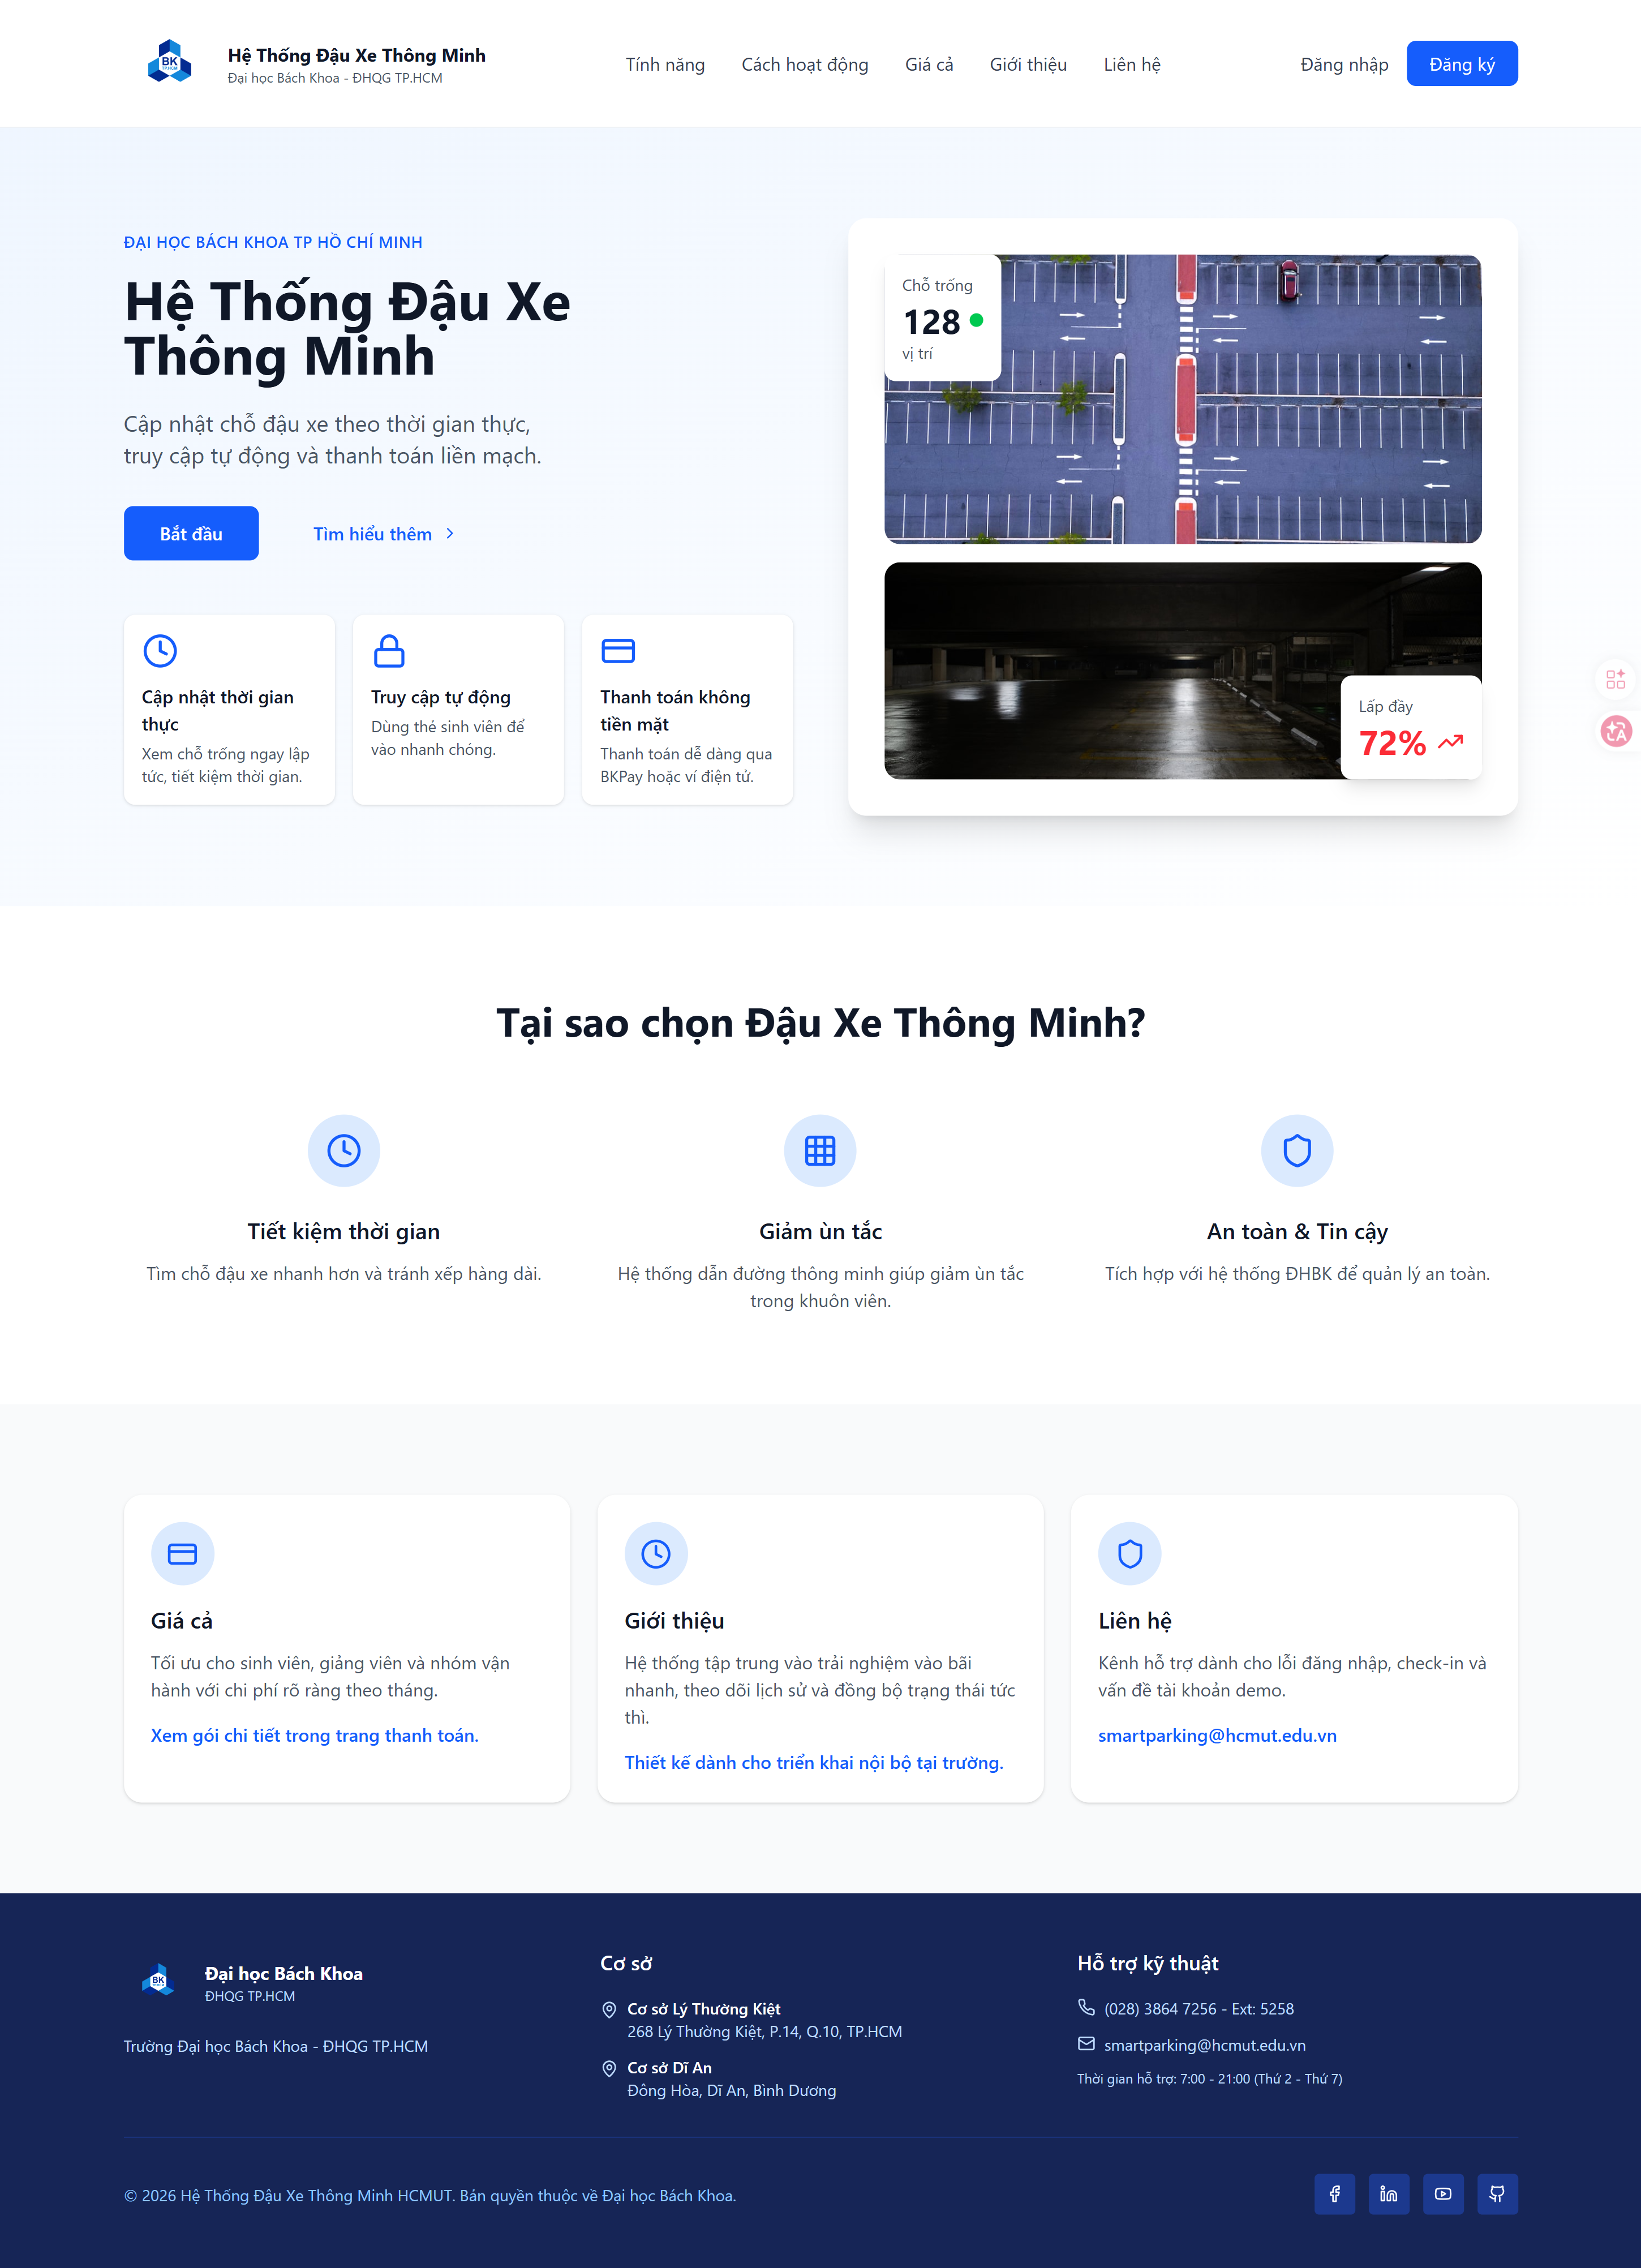
\includegraphics[width=1\linewidth]{Images/Task4/task4_home_overview.png} 
	\caption{Trang chủ của hệ thống Smart Parking}
\end{figure}

\textbf{Bước 2.} Khi chọn nút bắt đầu, hệ thống chuyển sang trang đăng nhập. Tại đây người dùng có thể chọn đúng loại tài khoản gồm HCMUT, quản trị viên hoặc nhân viên vận hành.

\begin{figure}[H]
	\centering
	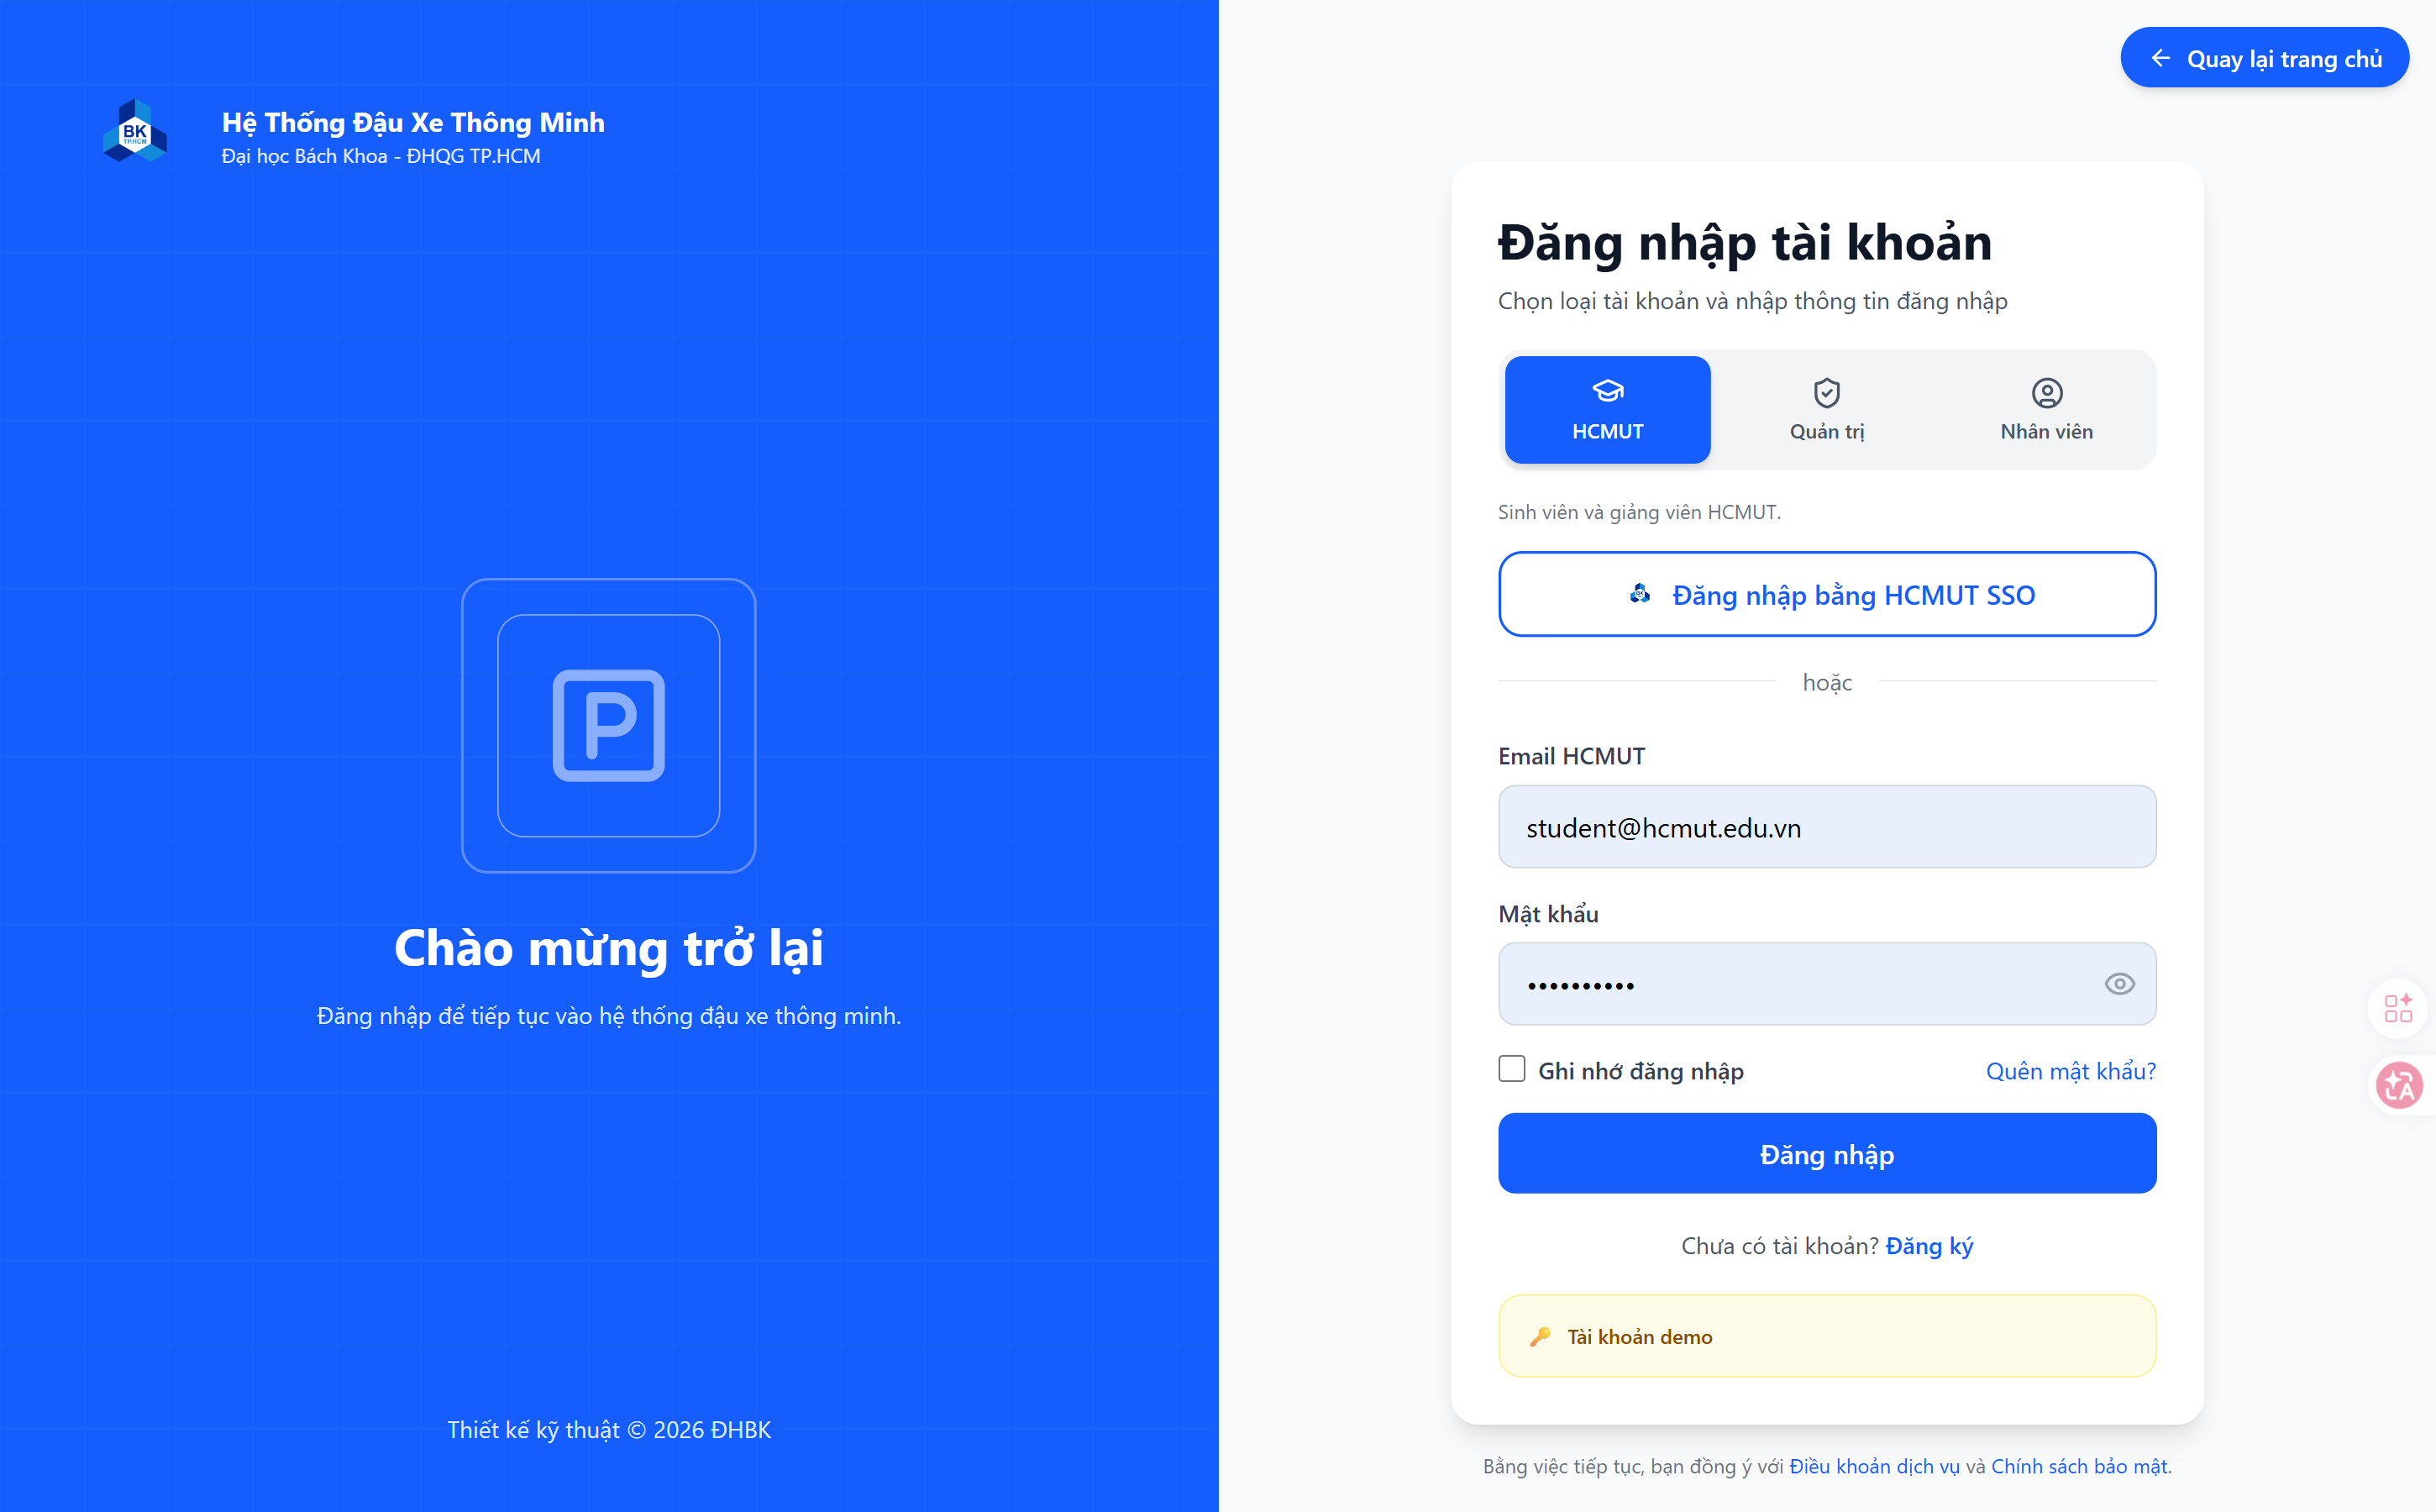
\includegraphics[width=1\linewidth]{Images/Task4/task4_login_role_selection.png} 
	\caption{Trang đăng nhập với lựa chọn loại tài khoản}
\end{figure}

\subsubsection{Chuỗi màn hình 2: Luồng sinh viên đăng nhập và theo dõi trạng thái bãi xe}

\textbf{Bước 1.} Sinh viên chọn nhóm tài khoản HCMUT, nhập thông tin đăng nhập hoặc dùng tài khoản demo để vào hệ thống.

\begin{figure}[H]
	\centering
	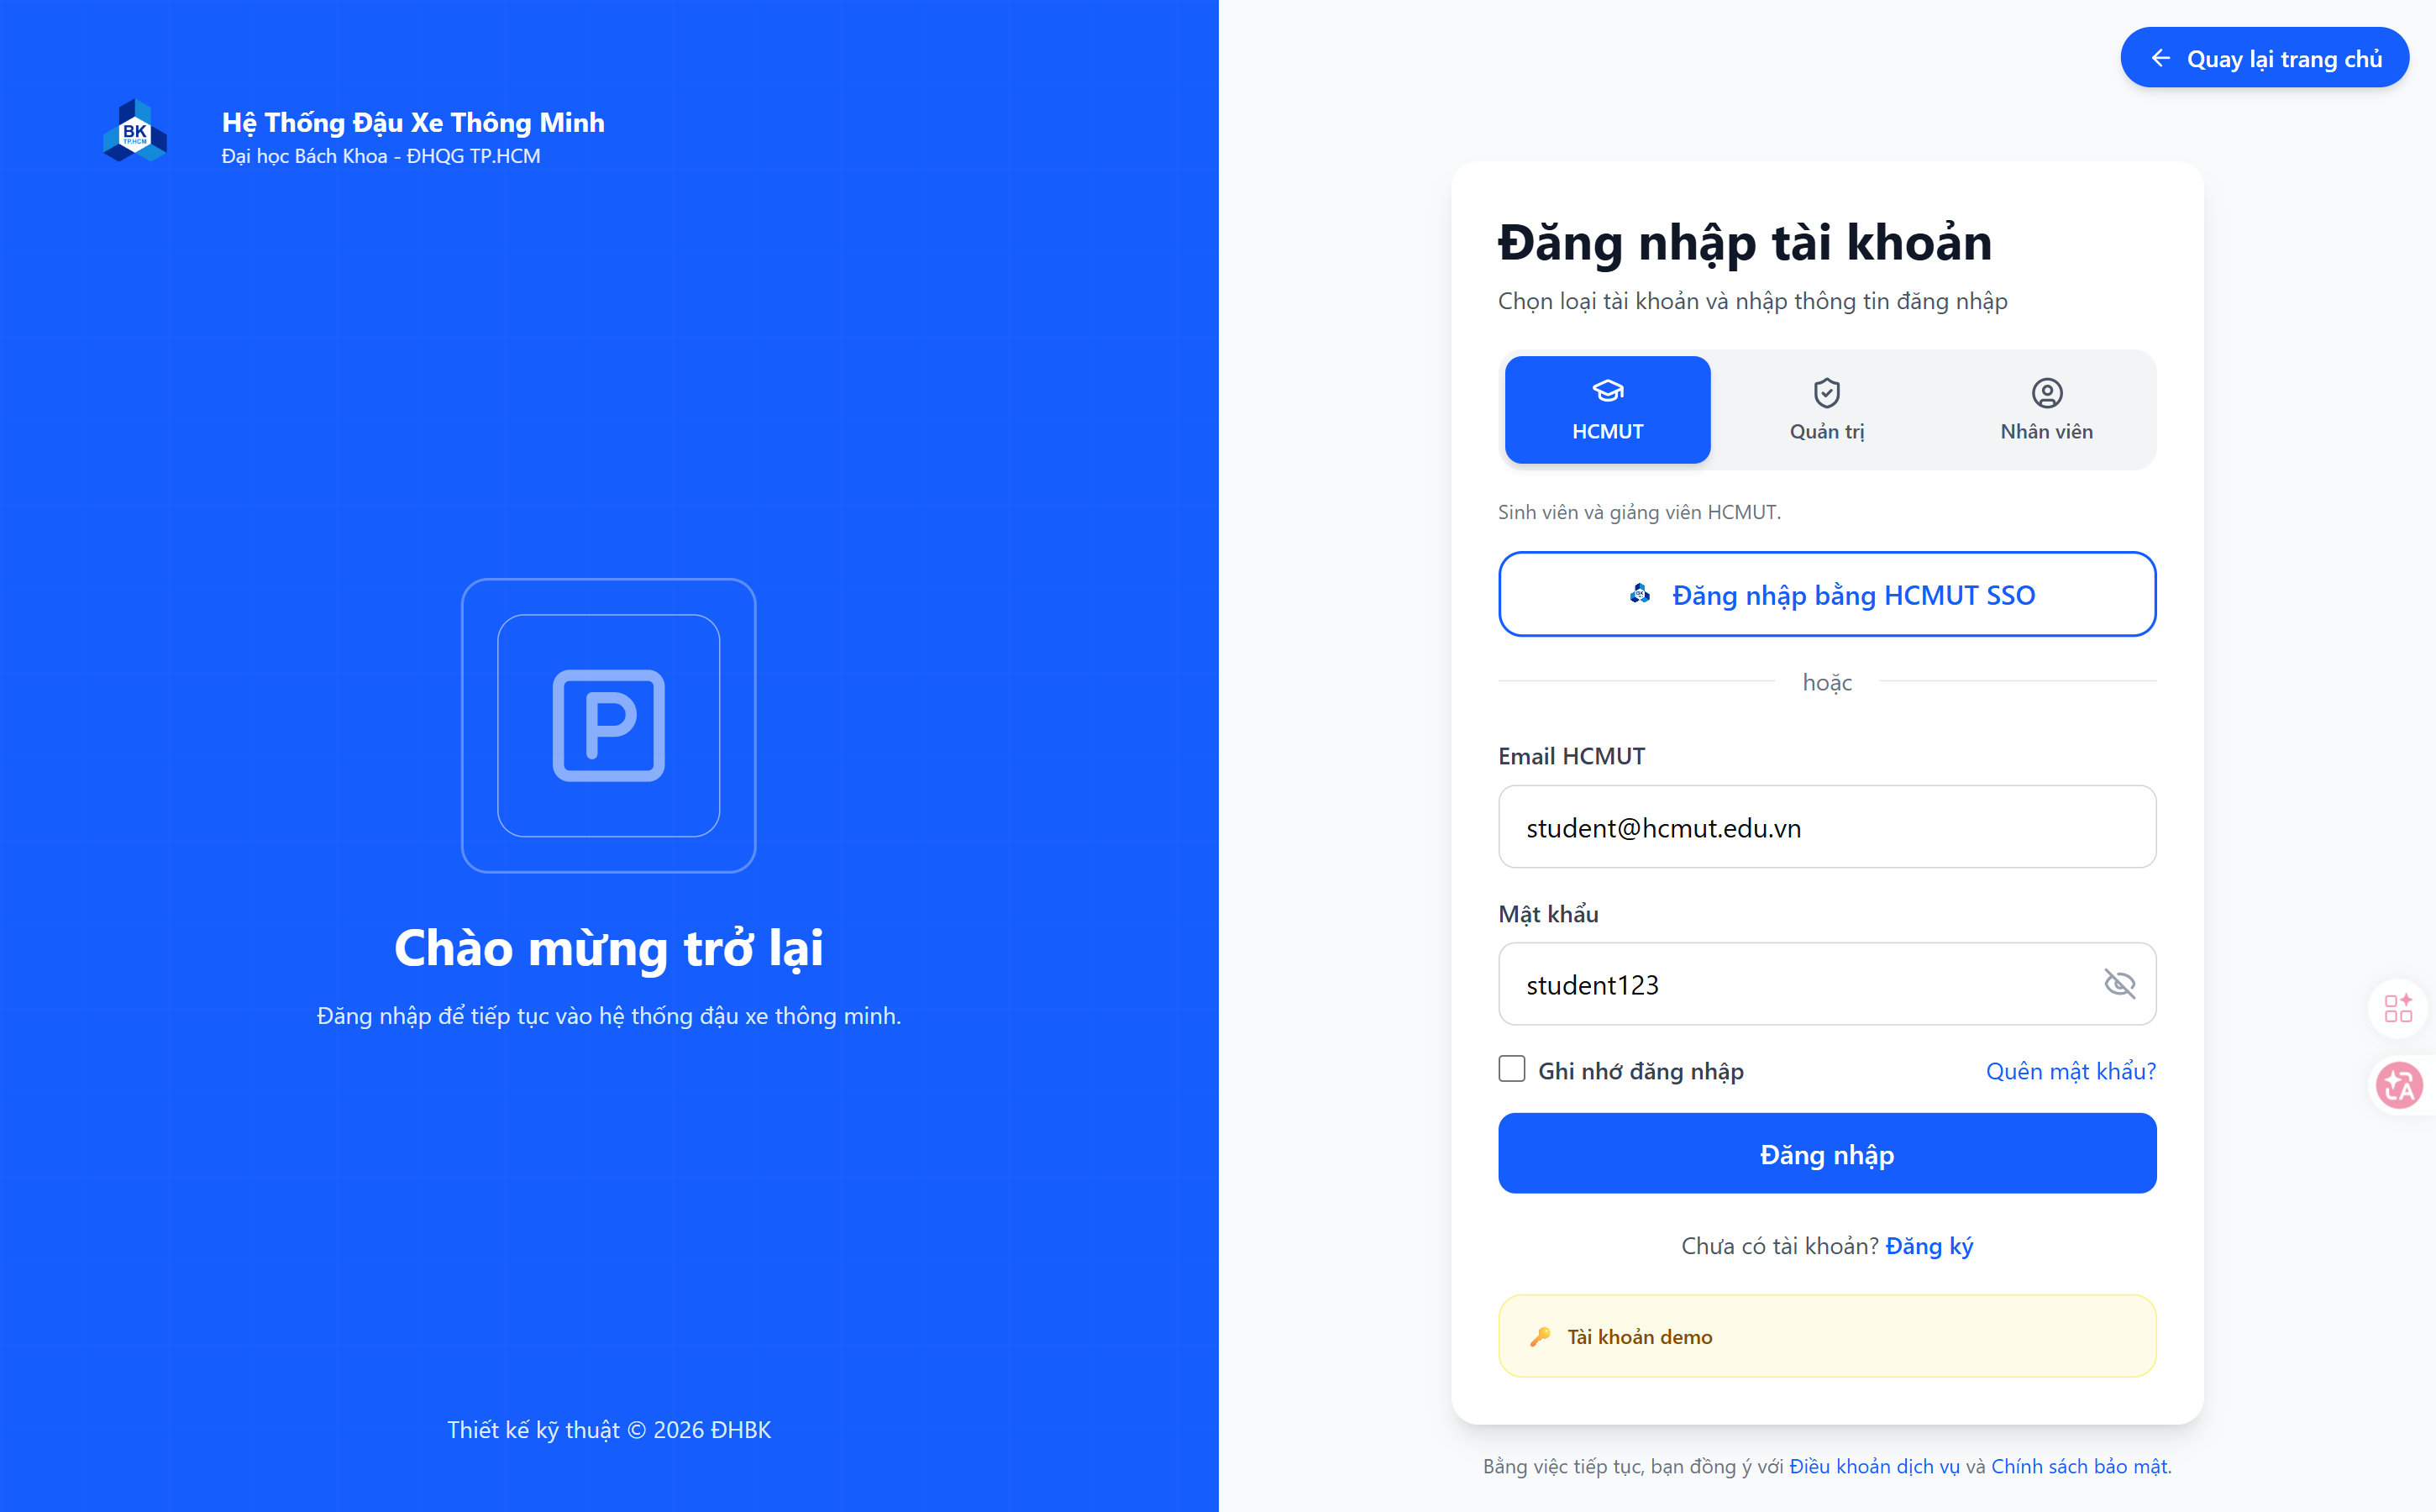
\includegraphics[width=1\linewidth]{Images/Task4/task4_student_login.png} 
	\caption{Sinh viên đăng nhập vào hệ thống}
\end{figure}

\textbf{Bước 2.} Sau khi đăng nhập thành công, hệ thống hiển thị dashboard của sinh viên. Màn hình này cho biết số chỗ trống, vai trò người dùng, trạng thái gói gửi xe, sơ đồ bãi đậu xe, tần suất đăng nhập và các hoạt động gần đây.

\begin{figure}[H]
	\centering
	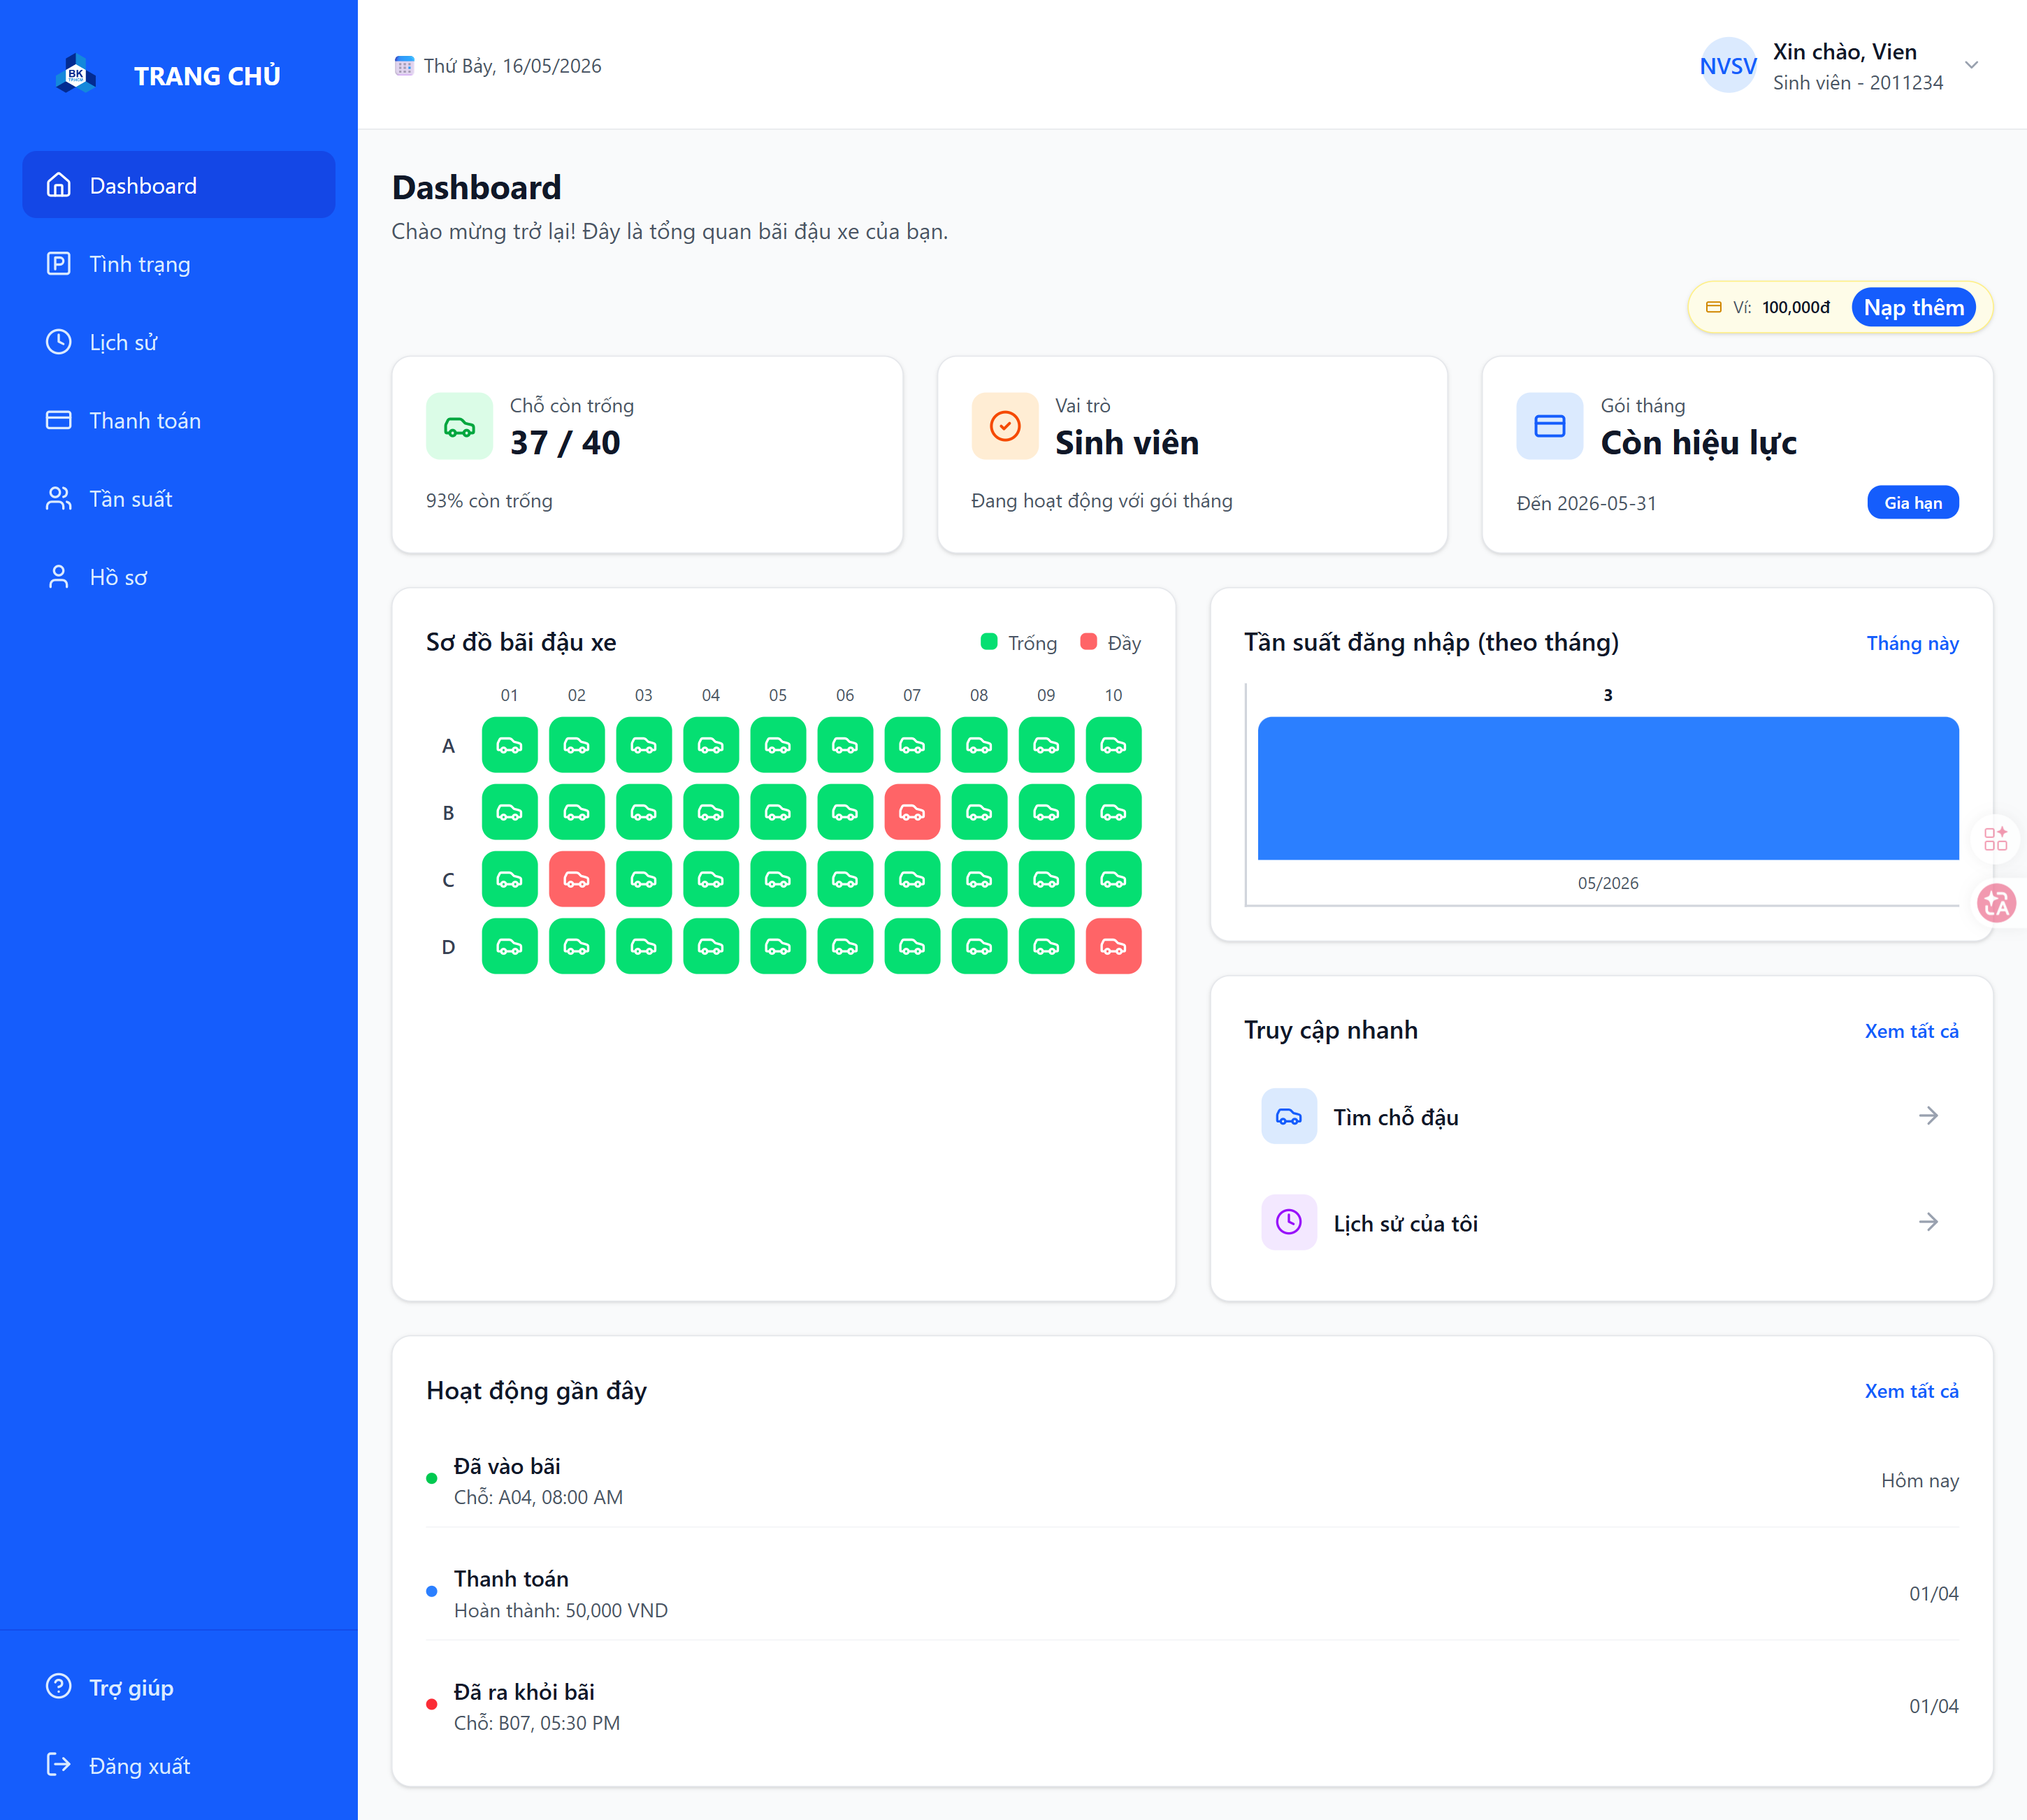
\includegraphics[width=1\linewidth]{Images/Task4/task4_student_dashboard.png} 
	\caption{Dashboard của sinh viên sau khi đăng nhập}
\end{figure}

\textbf{Bước 3.} Từ dashboard, sinh viên mở trang tình trạng bãi để xem sơ đồ các khu A, B, C, D. Các ô được phân biệt rõ giữa trạng thái còn trống, đã đầy và vị trí đang được gán cho người dùng.

\begin{figure}[H]
	\centering
	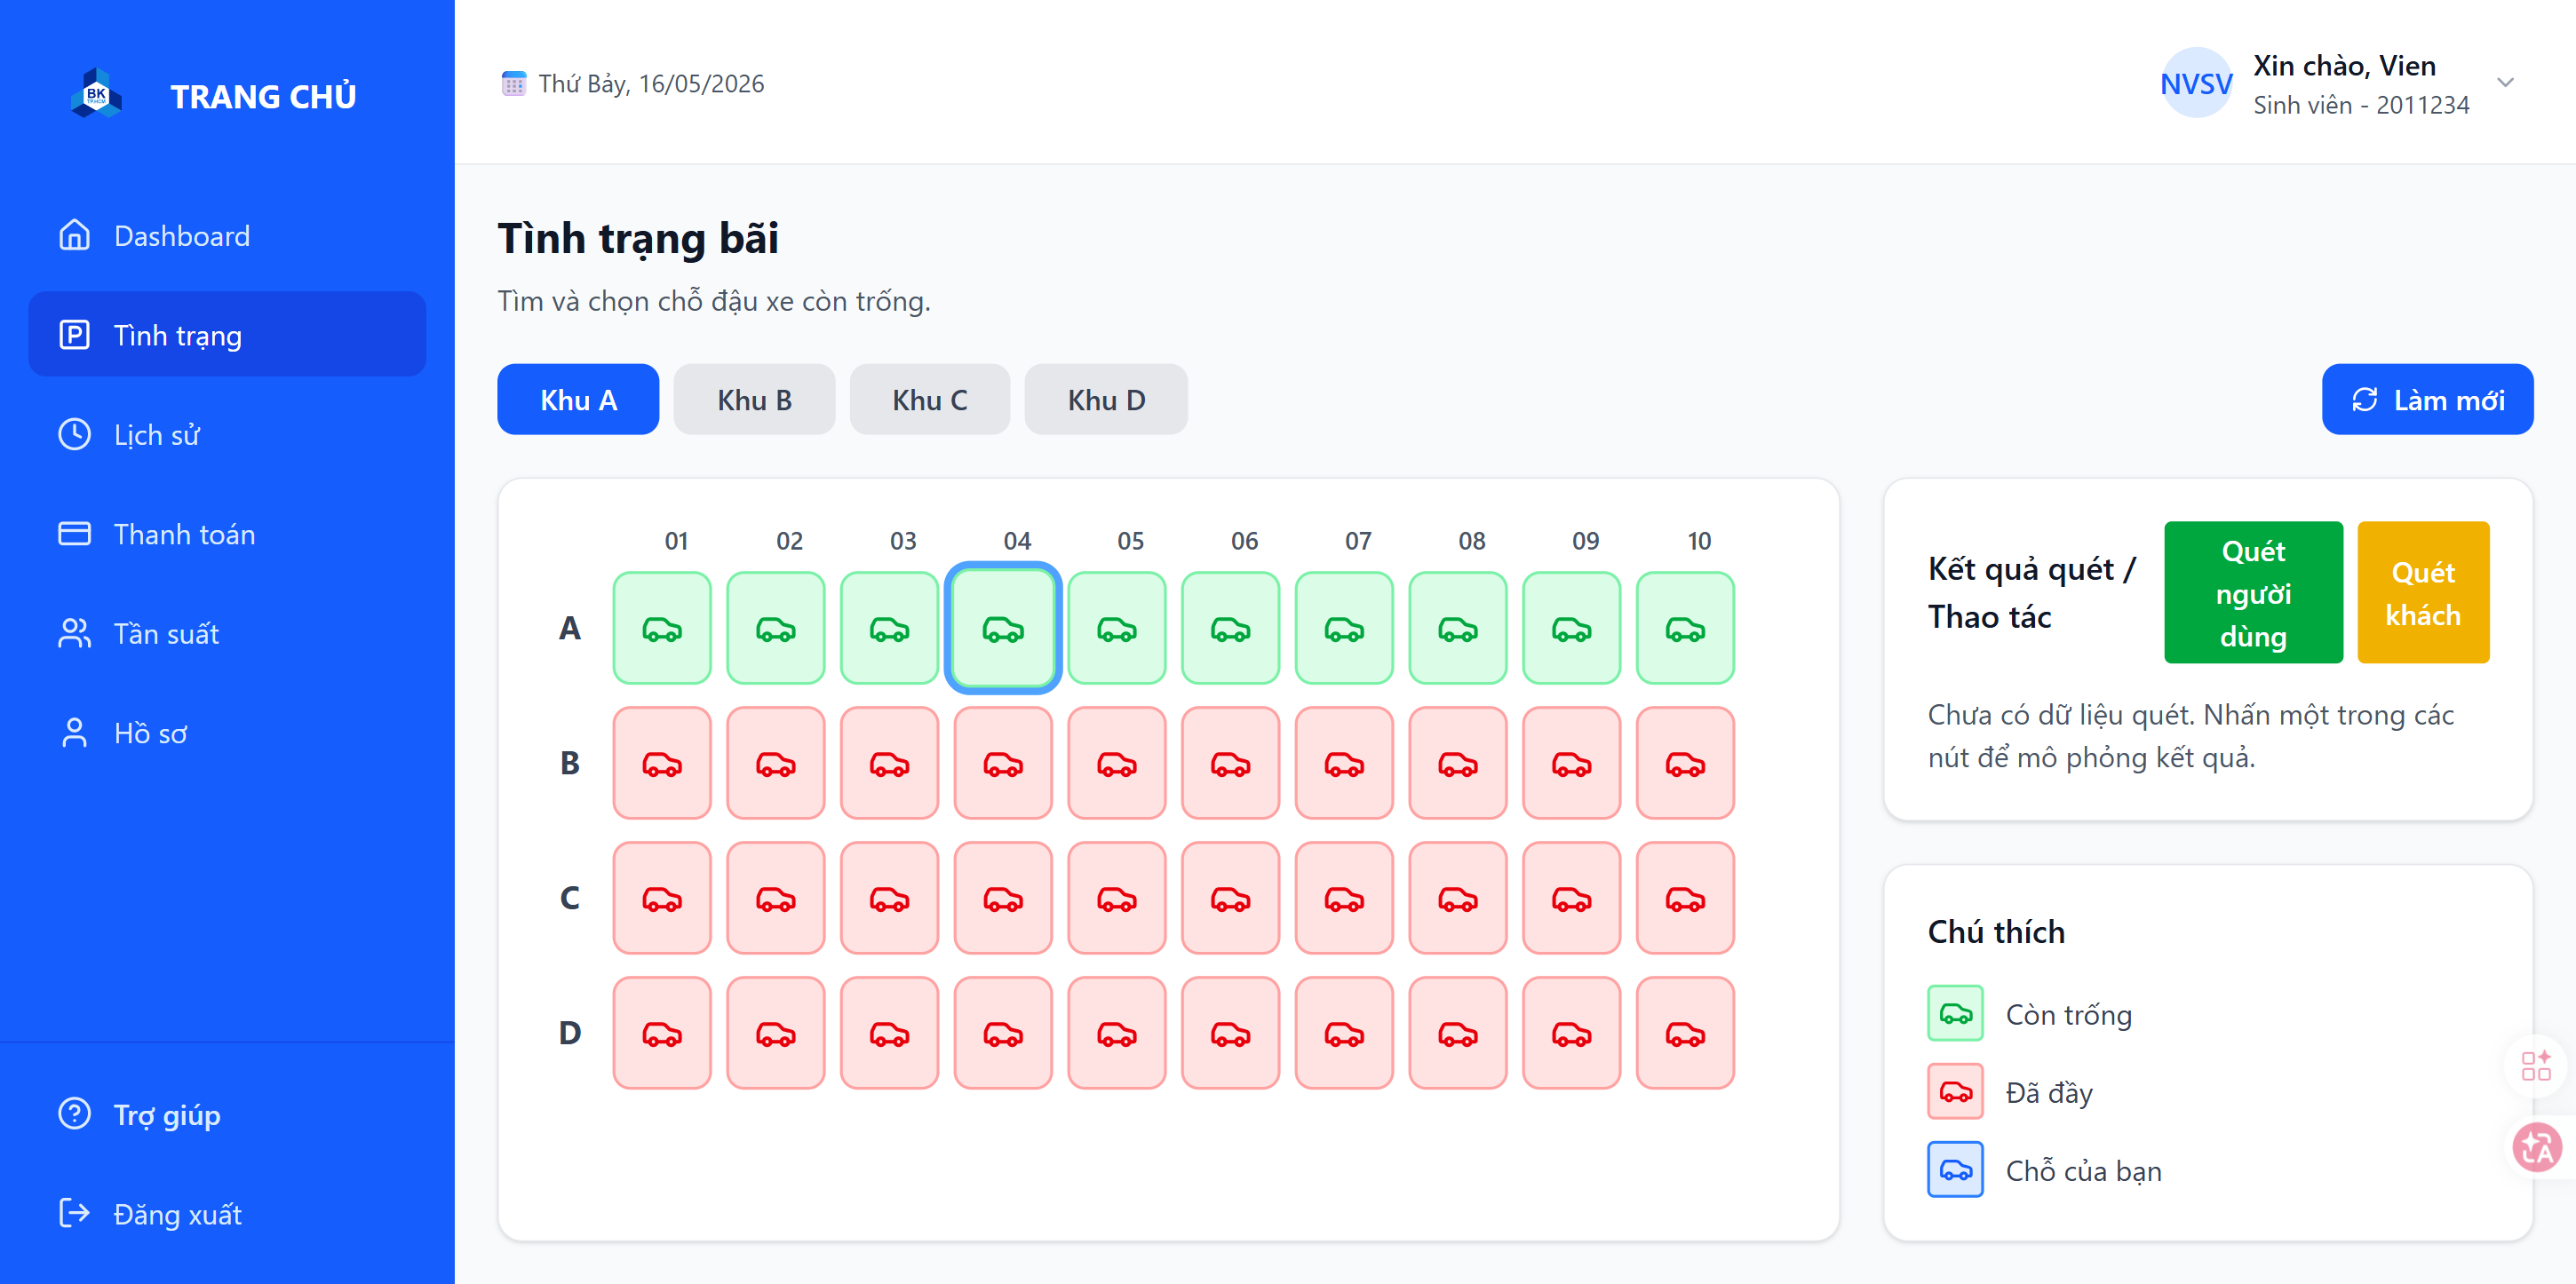
\includegraphics[width=1\linewidth]{Images/Task4/task4_student_parking_map.png} 
	\caption{Trang tình trạng bãi xe với sơ đồ các vị trí đậu}
\end{figure}

\textbf{Bước 4.} Ở cùng màn hình này, hệ thống còn mô phỏng kết quả quét thẻ nội bộ. Sau khi quét người dùng, hệ thống hiển thị thông tin cá nhân, biển số xe, giờ vào và vị trí được gán để minh họa luồng check-in nội bộ.

\begin{figure}[H]
	\centering
	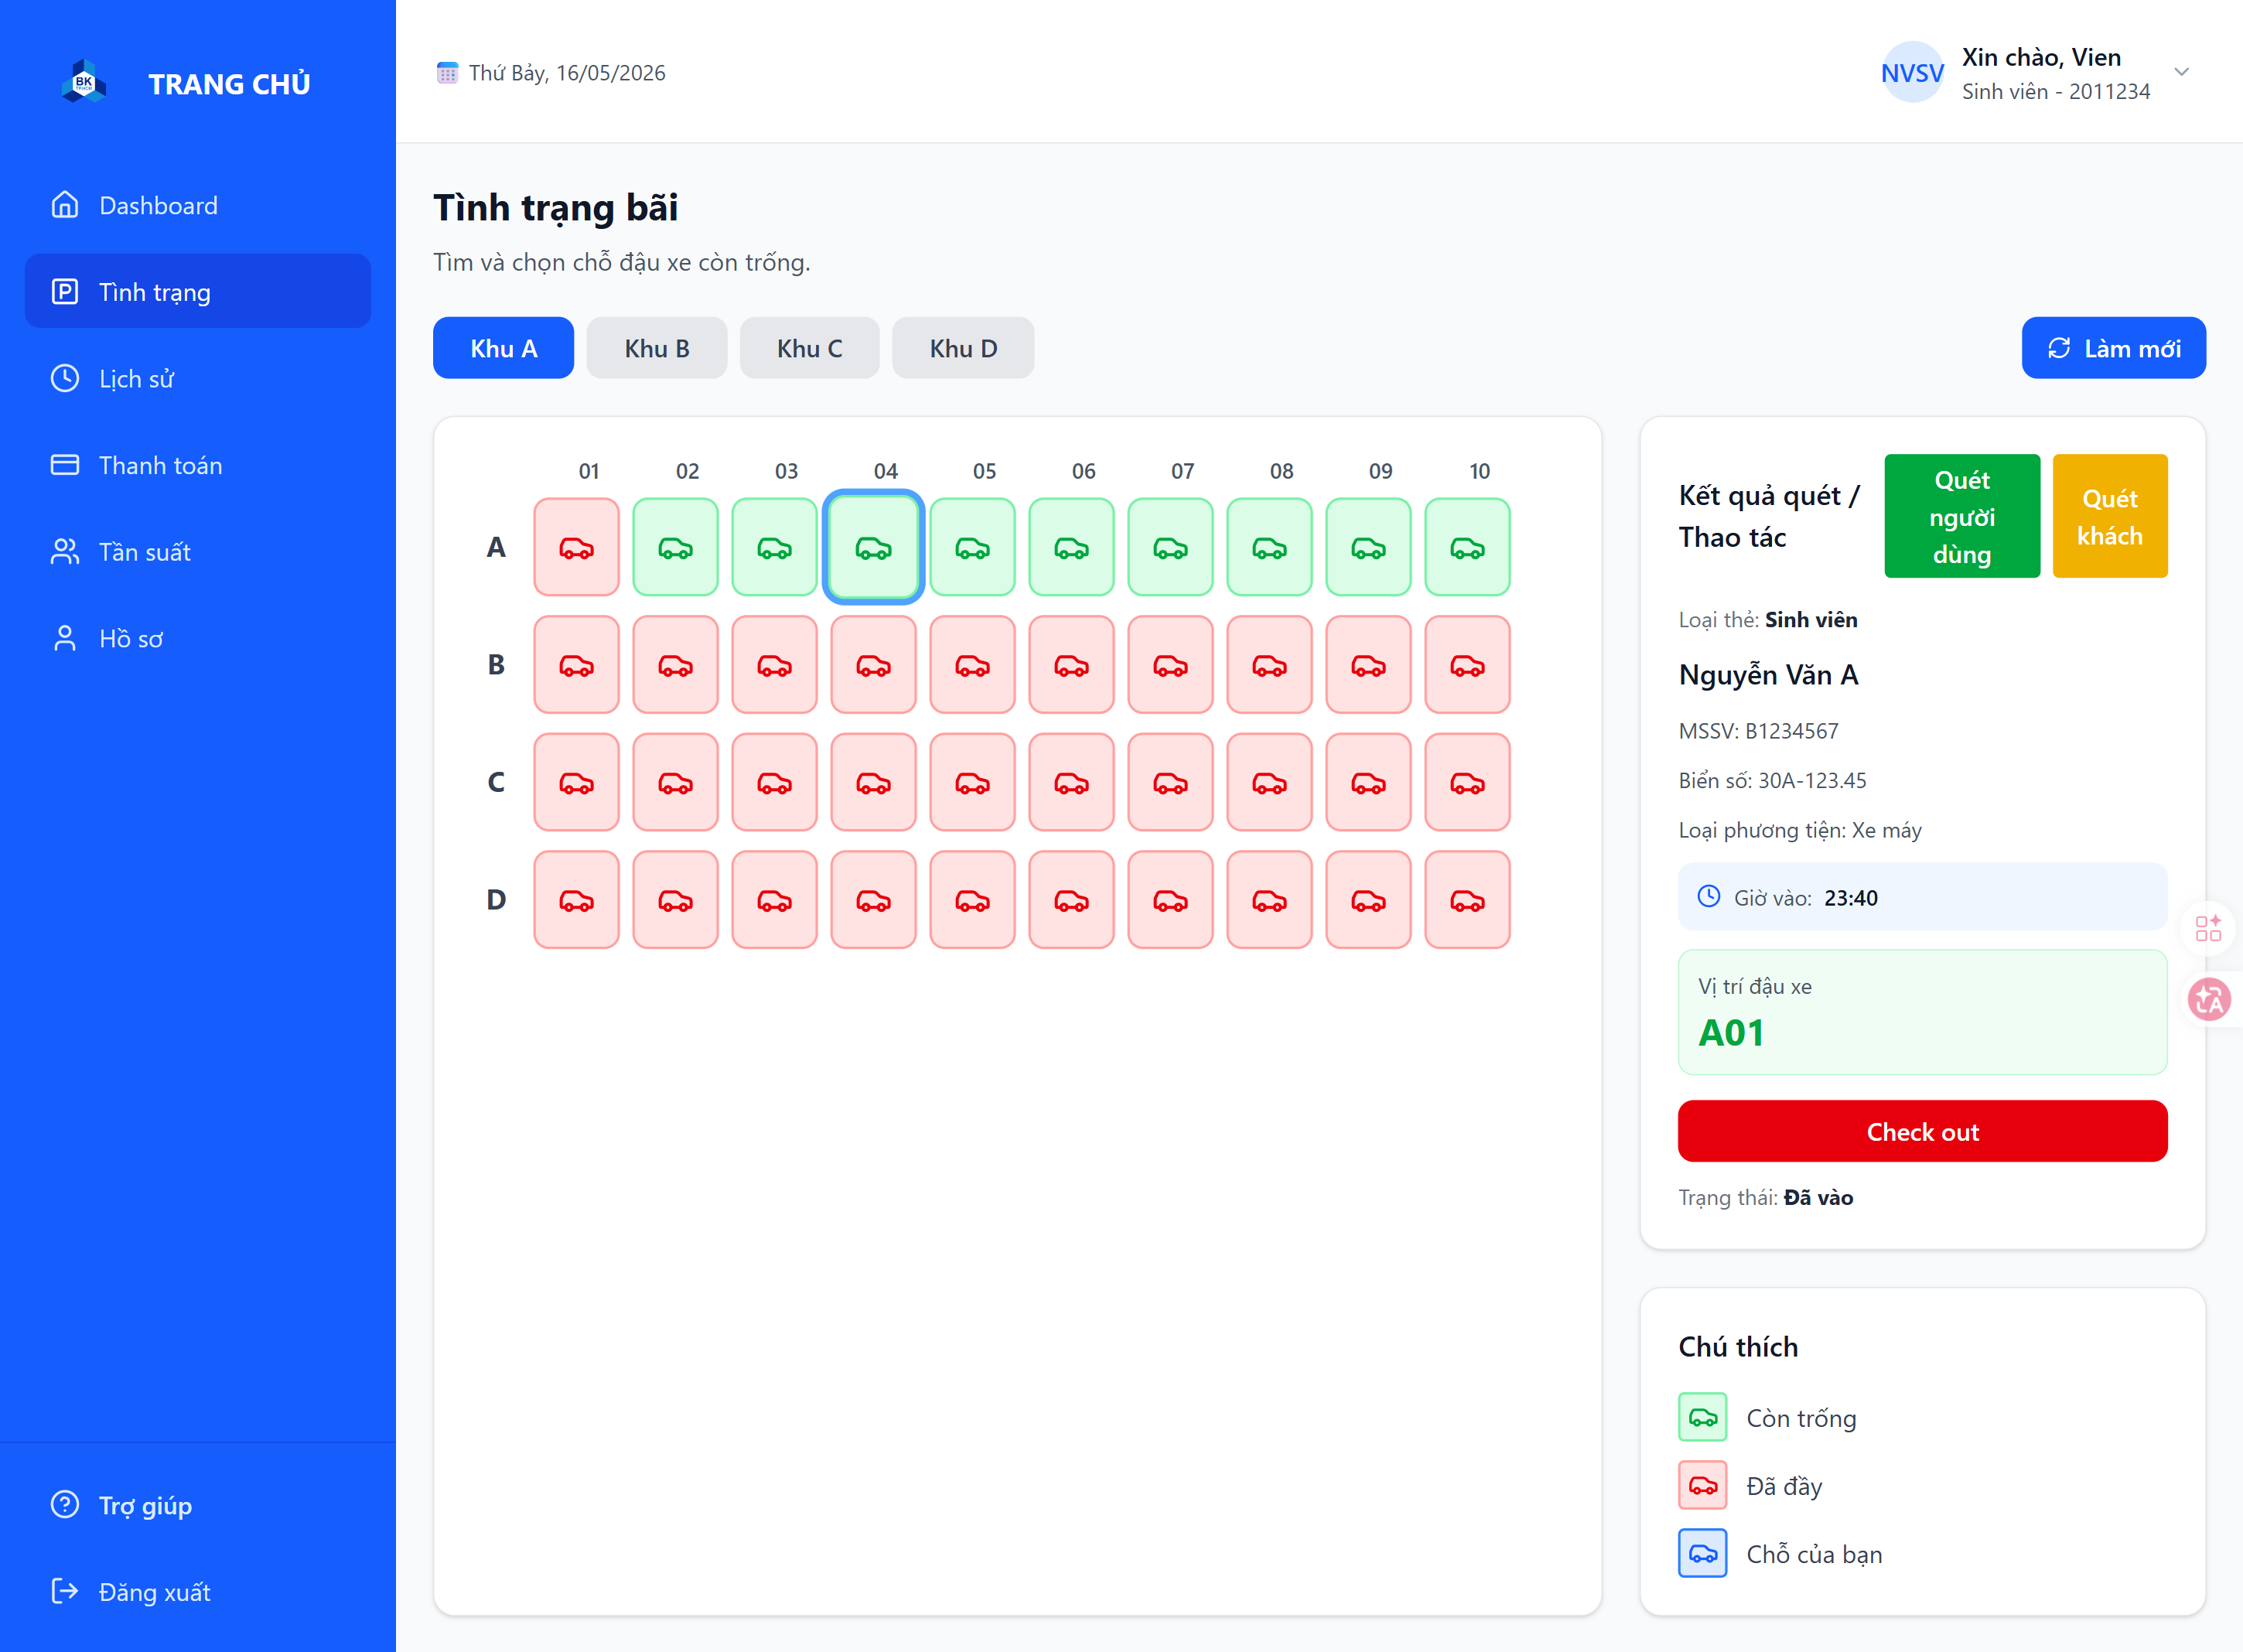
\includegraphics[width=1\linewidth]{Images/Task4/task4_student_checkin_result.png} 
	\caption{Kết quả quét thẻ nội bộ và gán chỗ đậu cho sinh viên}
\end{figure}

\textbf{Bước 5.} Khi rời bãi, người dùng tiếp tục thao tác check-out trên cùng khu vực mô phỏng. Hệ thống cập nhật giờ ra và kết thúc phiên gửi xe.

\begin{figure}[H]
	\centering
	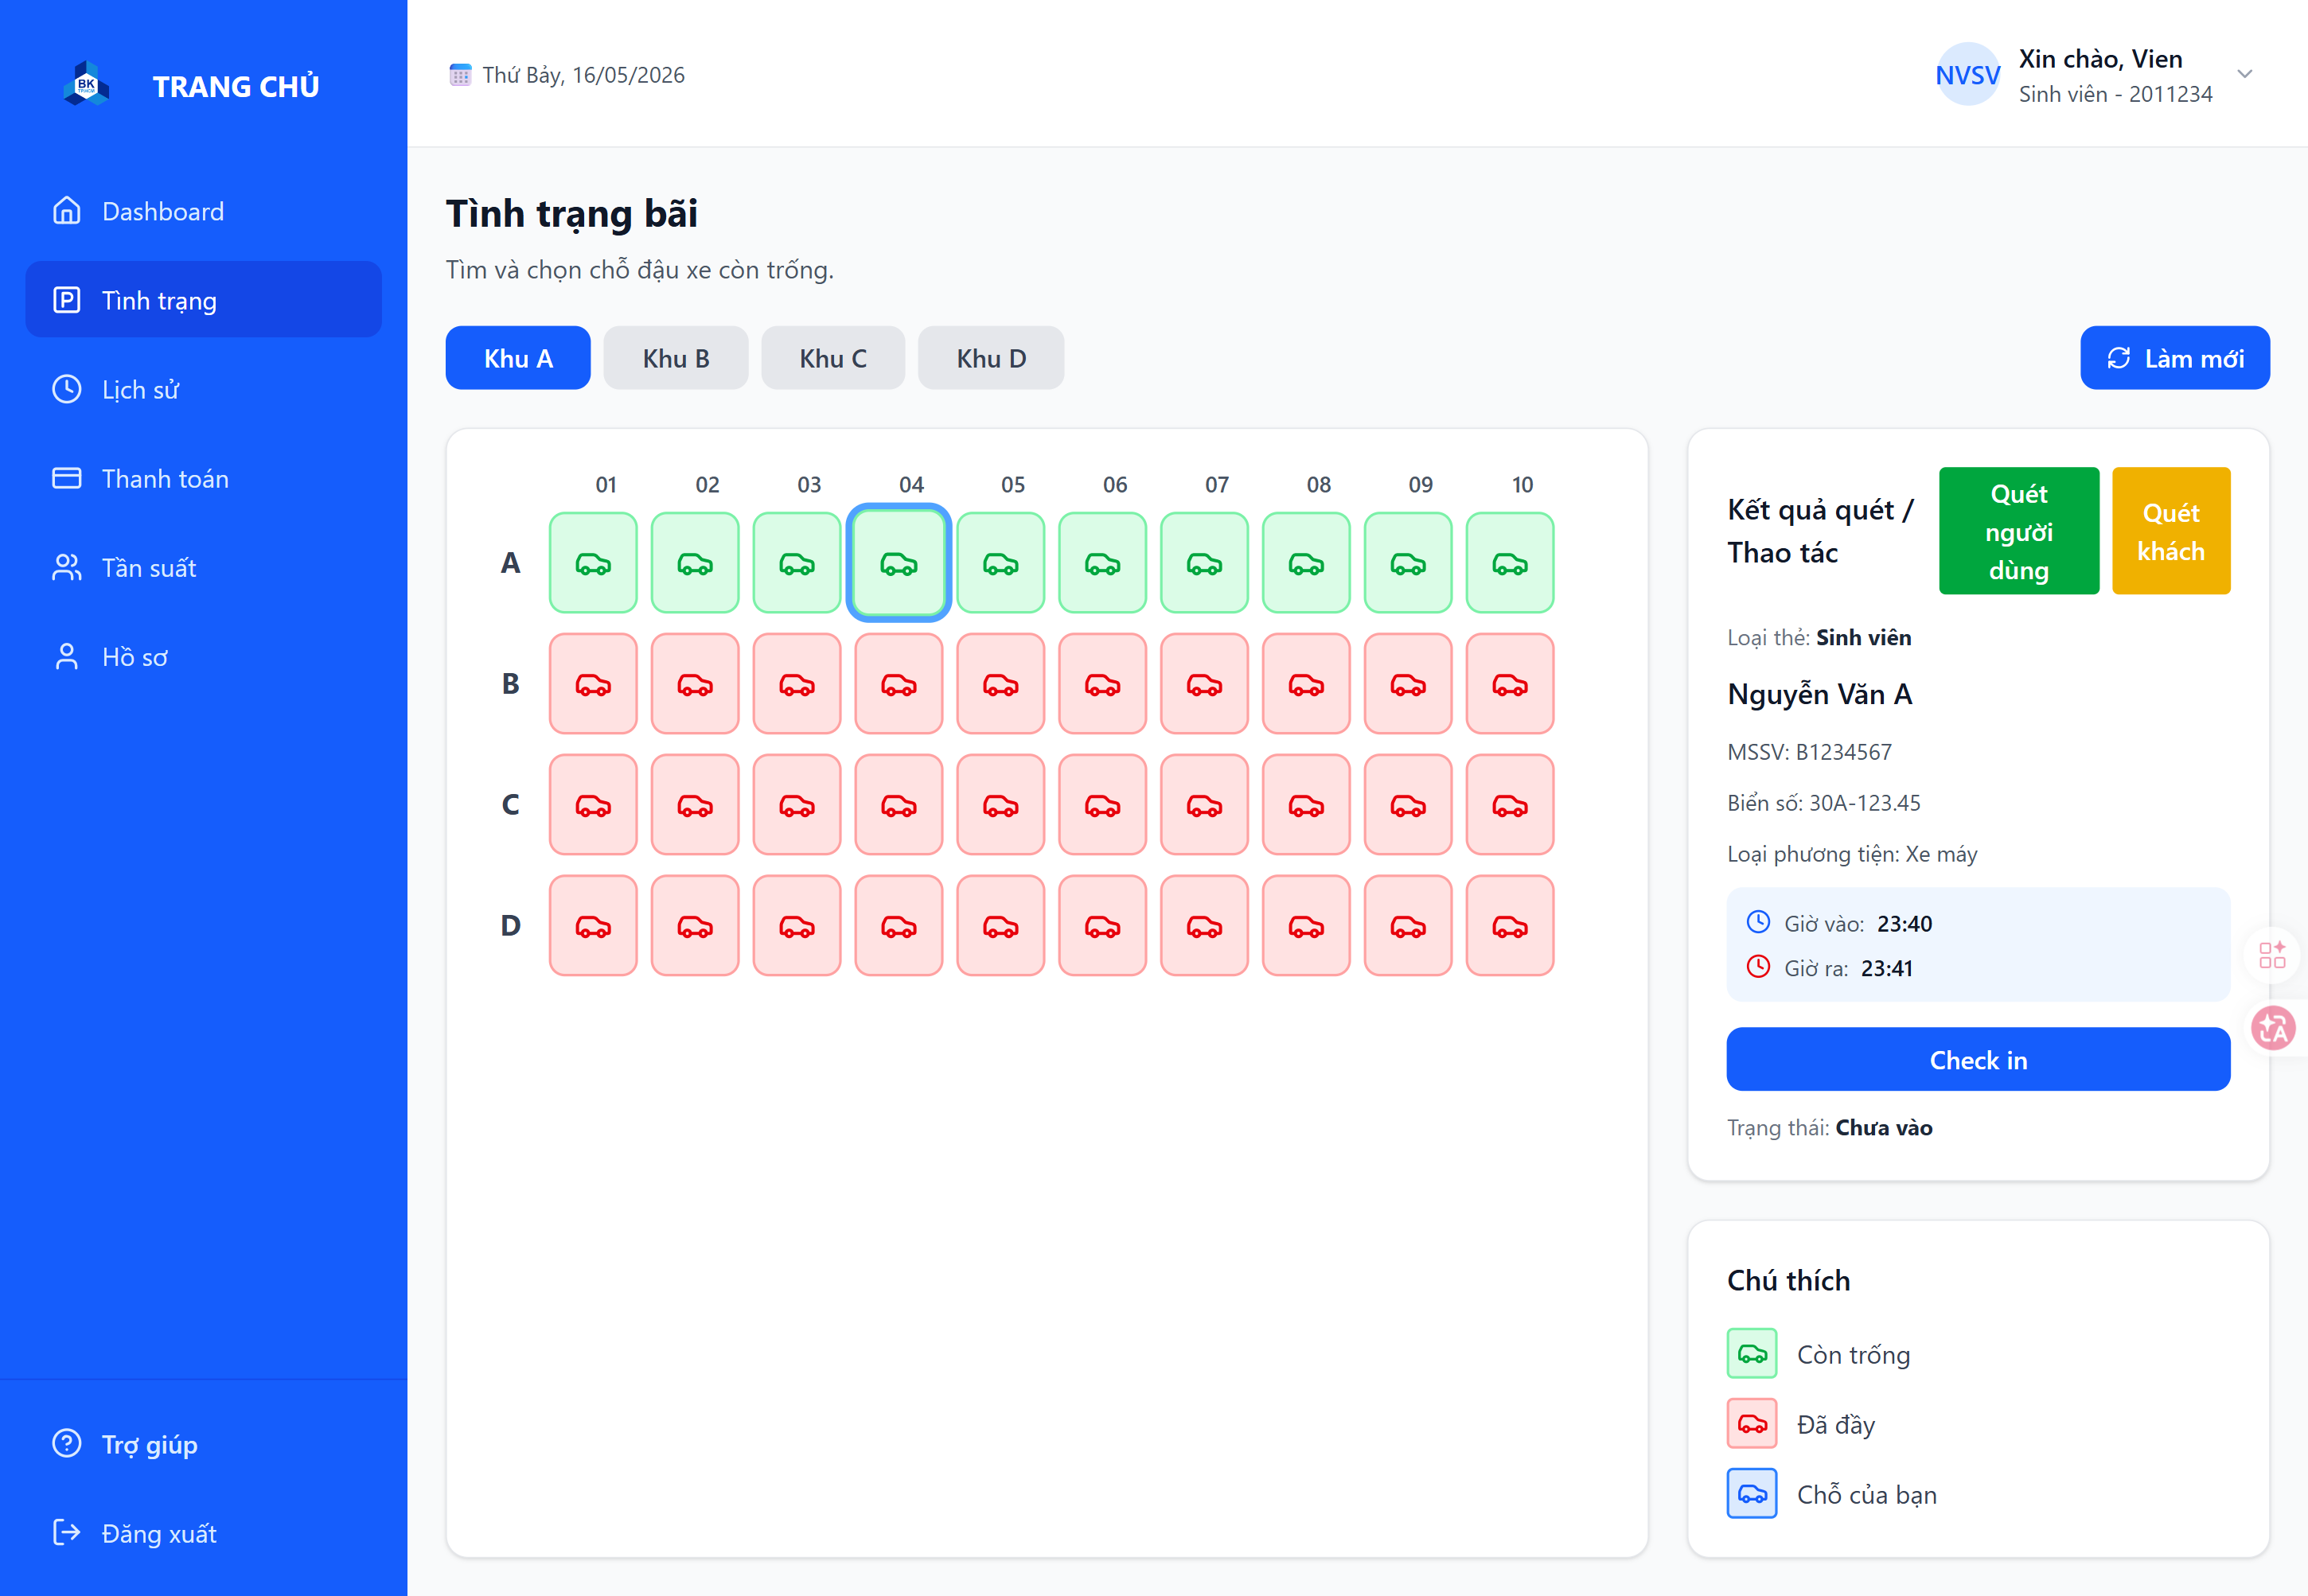
\includegraphics[width=1\linewidth]{Images/Task4/task4_student_checkout_result.png} 
	\caption{Màn hình minh họa check-out của người dùng nội bộ}
\end{figure}

\subsubsection{Chuỗi màn hình 3: Luồng sinh viên thanh toán gói gửi xe hàng tháng}

\textbf{Bước 1.} Sinh viên truy cập trang thanh toán để xem gói gửi xe hiện tại, thời gian hiệu lực và tổng chi phí cần thanh toán cho chu kỳ tháng.

\begin{figure}[H]
	\centering
	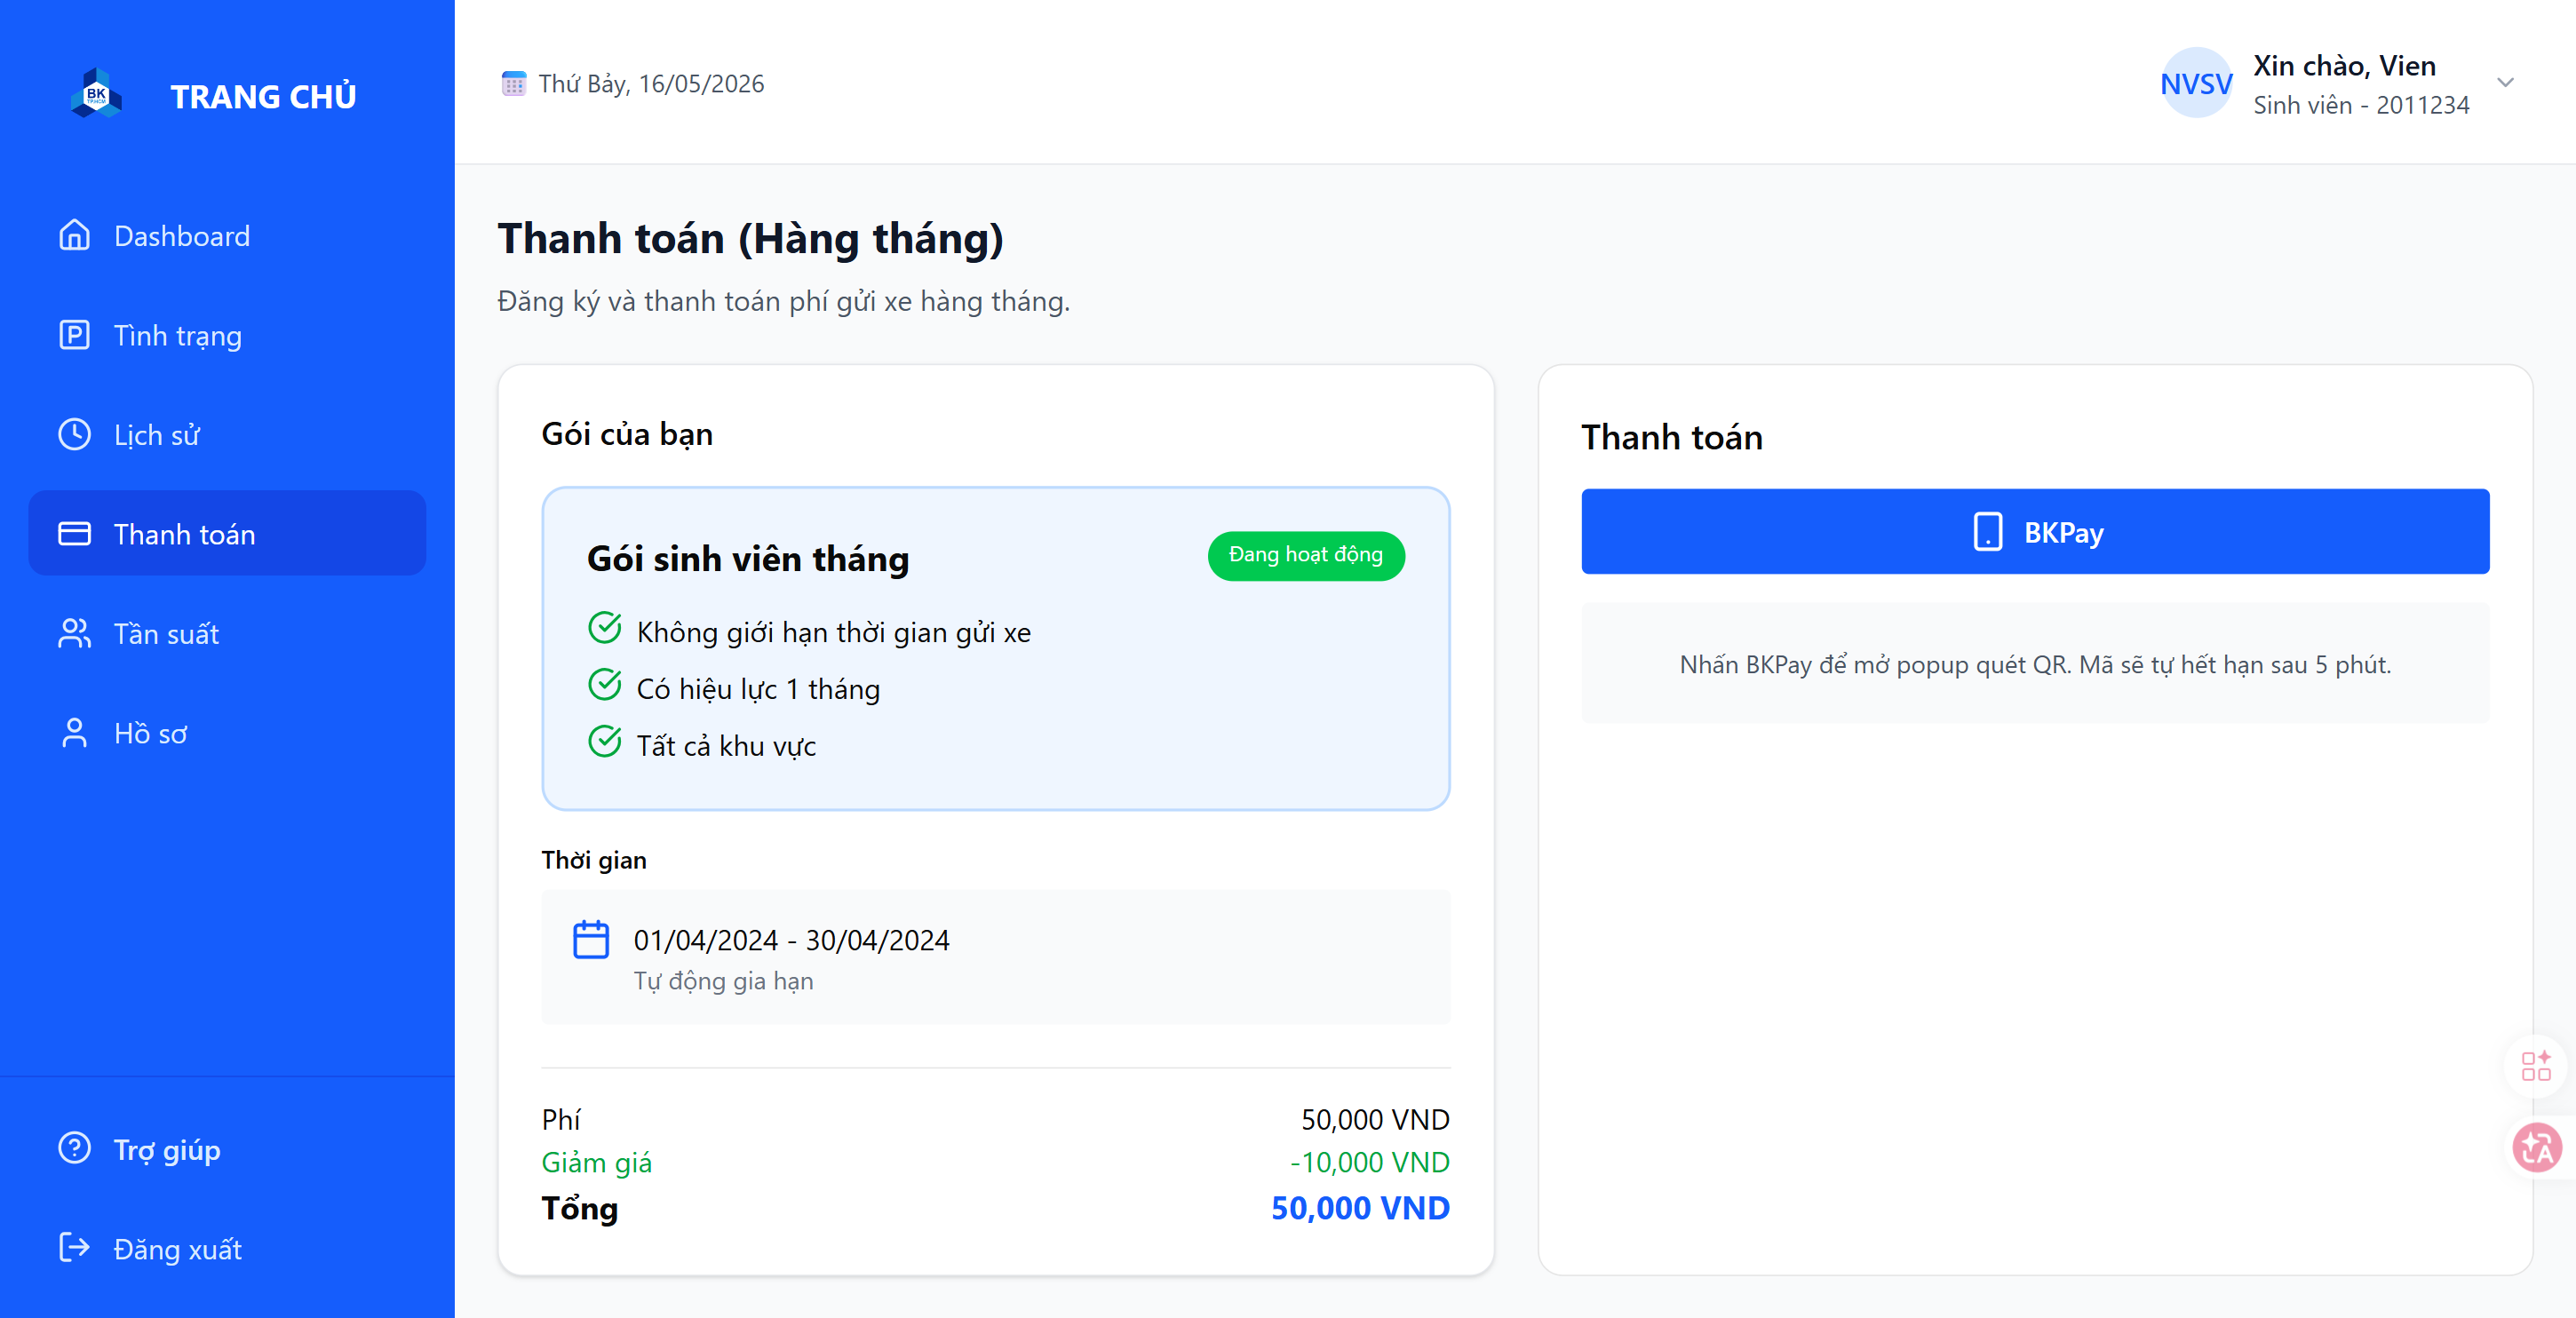
\includegraphics[width=1\linewidth]{Images/Task4/task4_student_payment_overview.png} 
	\caption{Trang thanh toán gói gửi xe hàng tháng của sinh viên}
\end{figure}

\textbf{Bước 2.} Khi nhấn BKPay, hệ thống mở cửa sổ thanh toán QR. Màn hình này thể hiện số tiền thanh toán, mã QR, thời gian hết hạn và nút xác nhận đã thanh toán.

\begin{figure}[H]
	\centering
	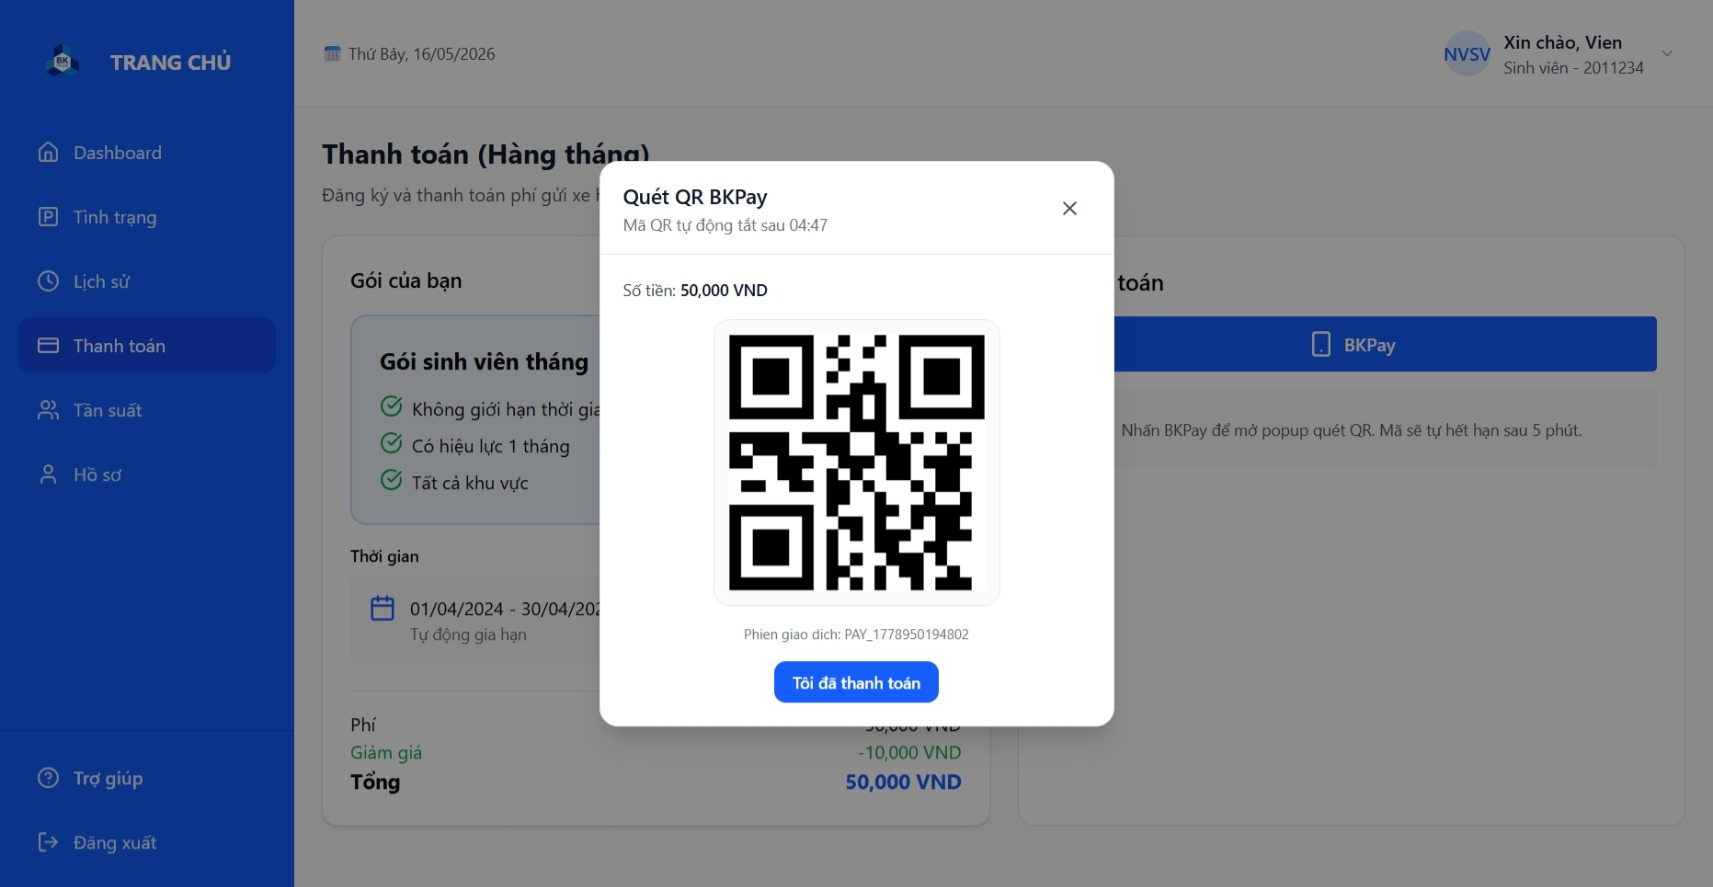
\includegraphics[width=1\linewidth]{Images/Task4/task4_student_bkpay_qr.jpeg} 
	\caption{Popup QR BKPay cho thanh toán gói tháng}
\end{figure}

\subsubsection{Chuỗi màn hình 4: Luồng sinh viên xem lịch sử và hồ sơ cá nhân}

\textbf{Bước 1.} Người dùng mở trang lịch sử để xem các phiên gửi xe đã phát sinh. Hệ thống hiển thị ngày, giờ vào, giờ ra, vị trí đậu, thời lượng, loại thẻ, mức phí và trạng thái giao dịch.

\begin{figure}[H]
	\centering
	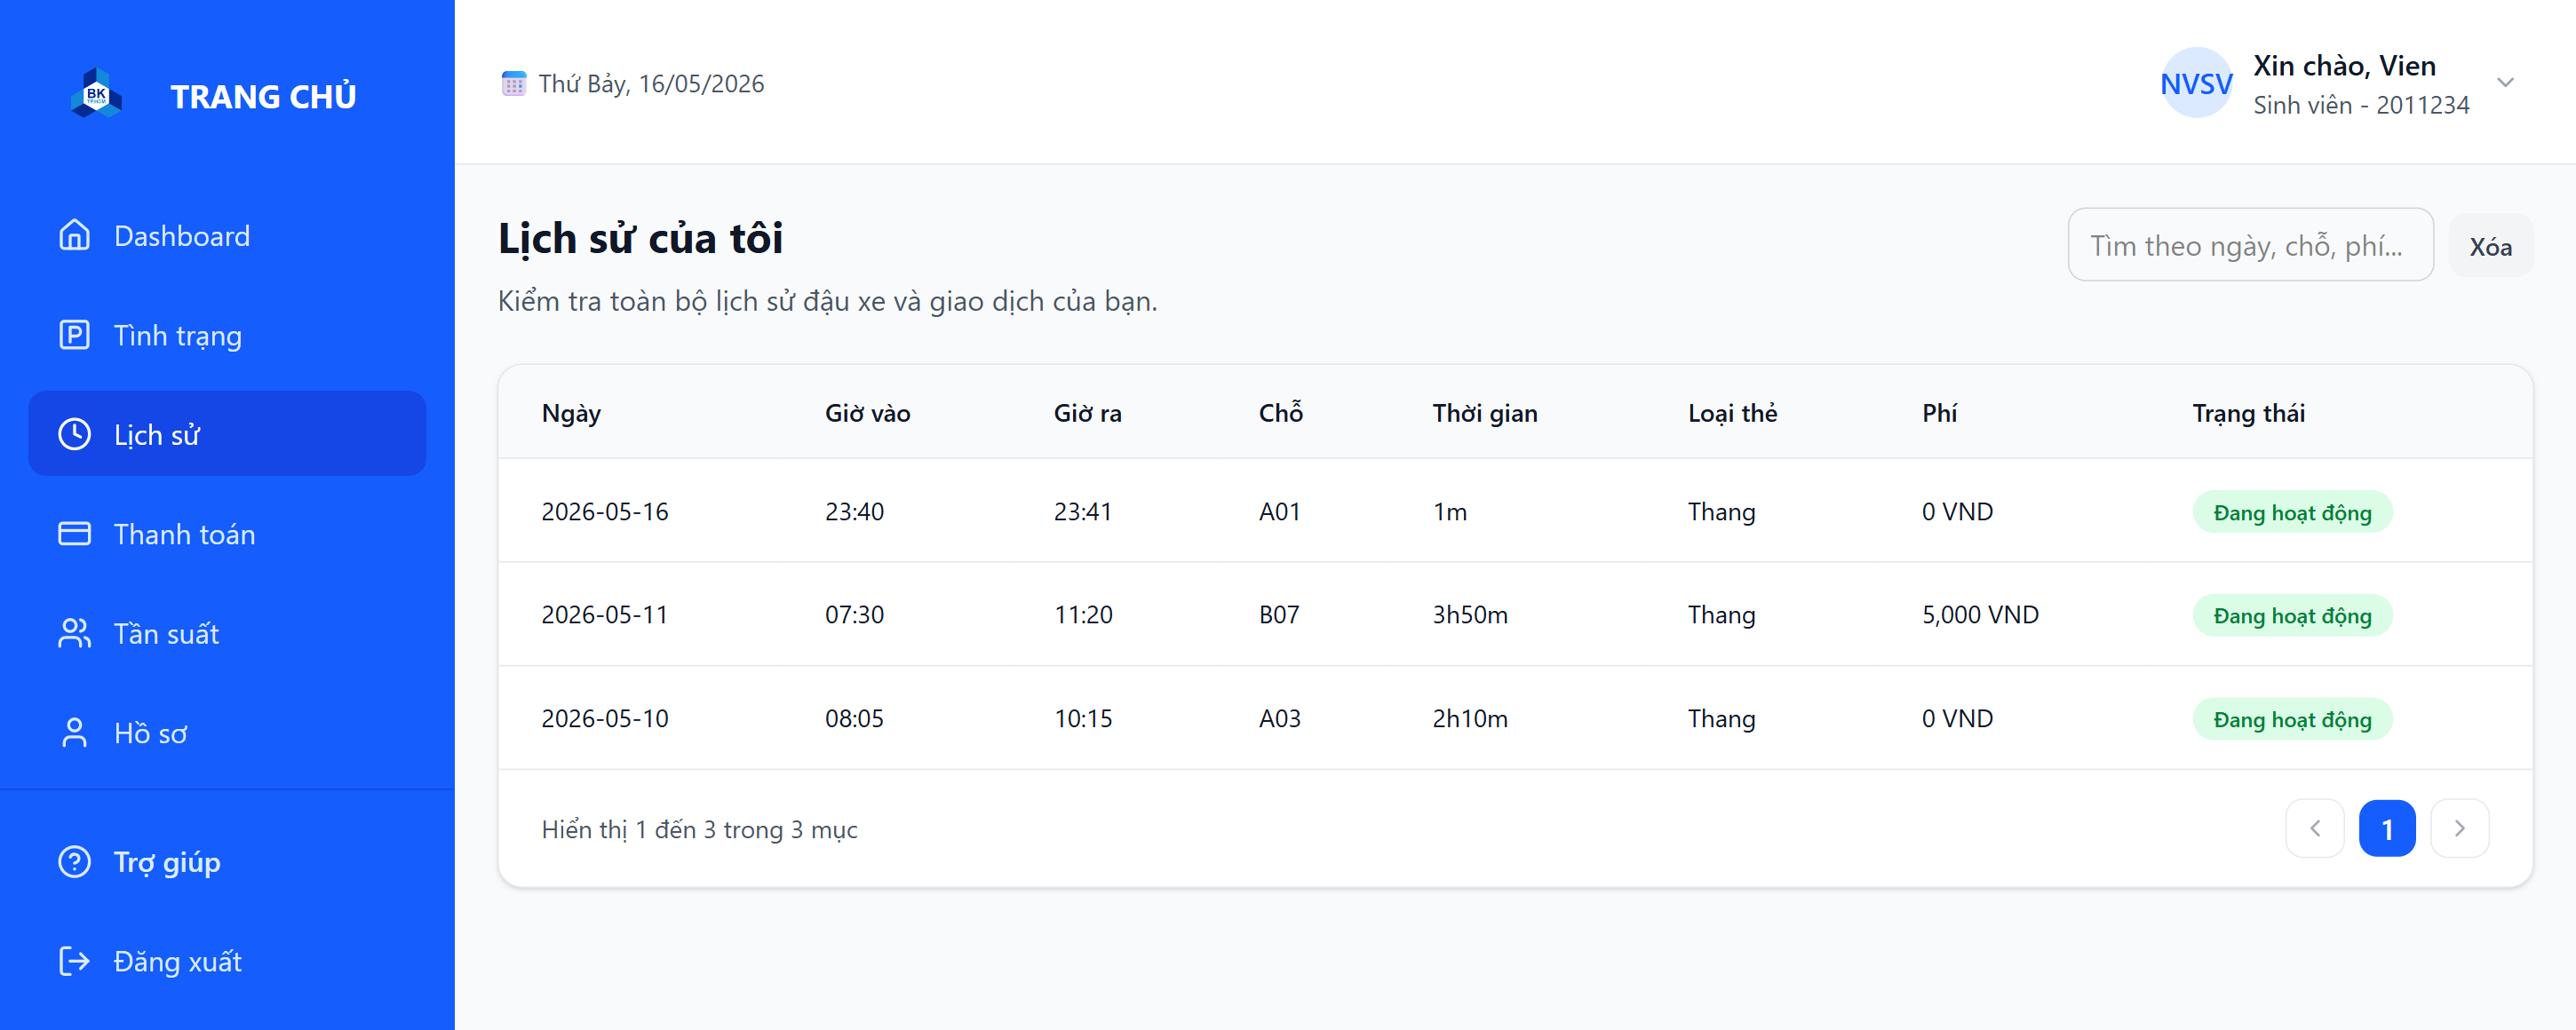
\includegraphics[width=1\linewidth]{Images/Task4/task4_student_history.png} 
	\caption{Trang lịch sử gửi xe của sinh viên}
\end{figure}

\textbf{Bước 2.} Người dùng tiếp tục vào trang hồ sơ để kiểm tra thông tin cá nhân, email, số điện thoại, biển số xe, mã định danh và các tùy chọn thông báo, bảo mật.

\begin{figure}[H]
	\centering
	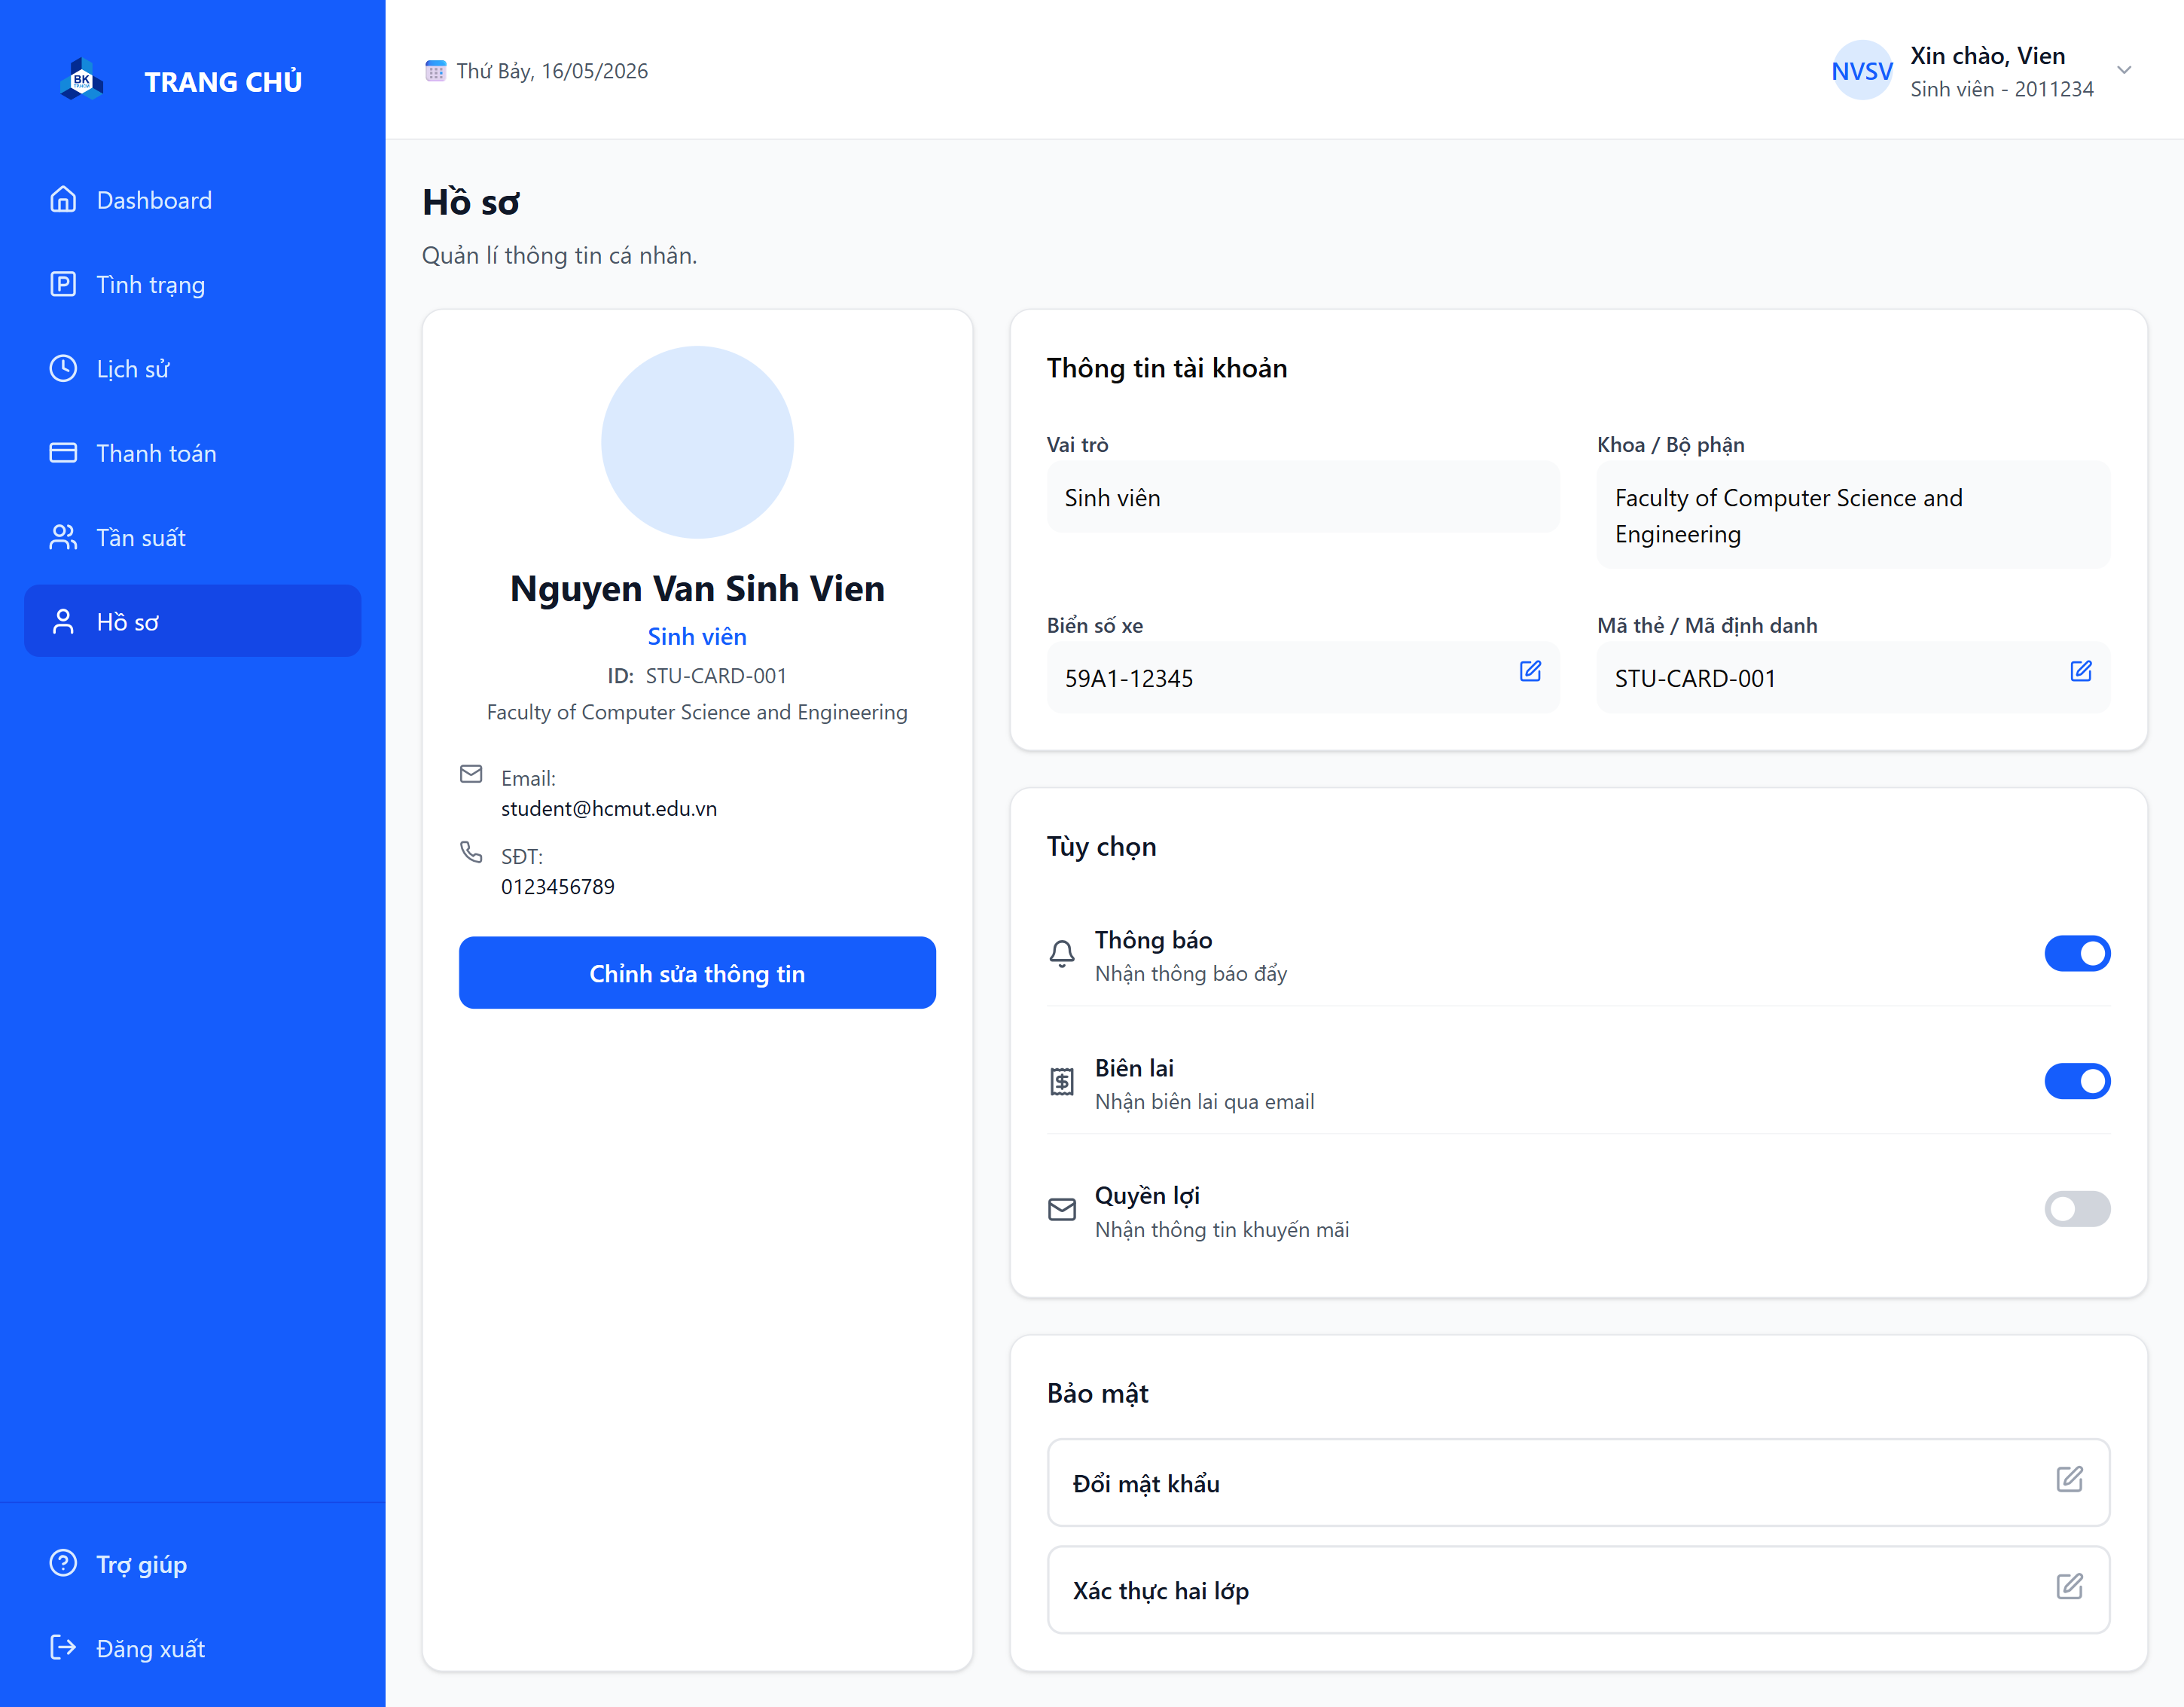
\includegraphics[width=1\linewidth]{Images/Task4/task4_student_profile.png} 
	\caption{Trang hồ sơ cá nhân của người dùng}
\end{figure}

\subsubsection{Chuỗi màn hình 5: Luồng giảng viên theo dõi giới hạn truy cập và mua thêm lượt}

\textbf{Bước 1.} Giảng viên đăng nhập bằng tài khoản HCMUT và được chuyển đến dashboard có thông tin số chỗ trống cùng thẻ thống kê giới hạn truy cập theo tháng.

\begin{figure}[H]
	\centering
	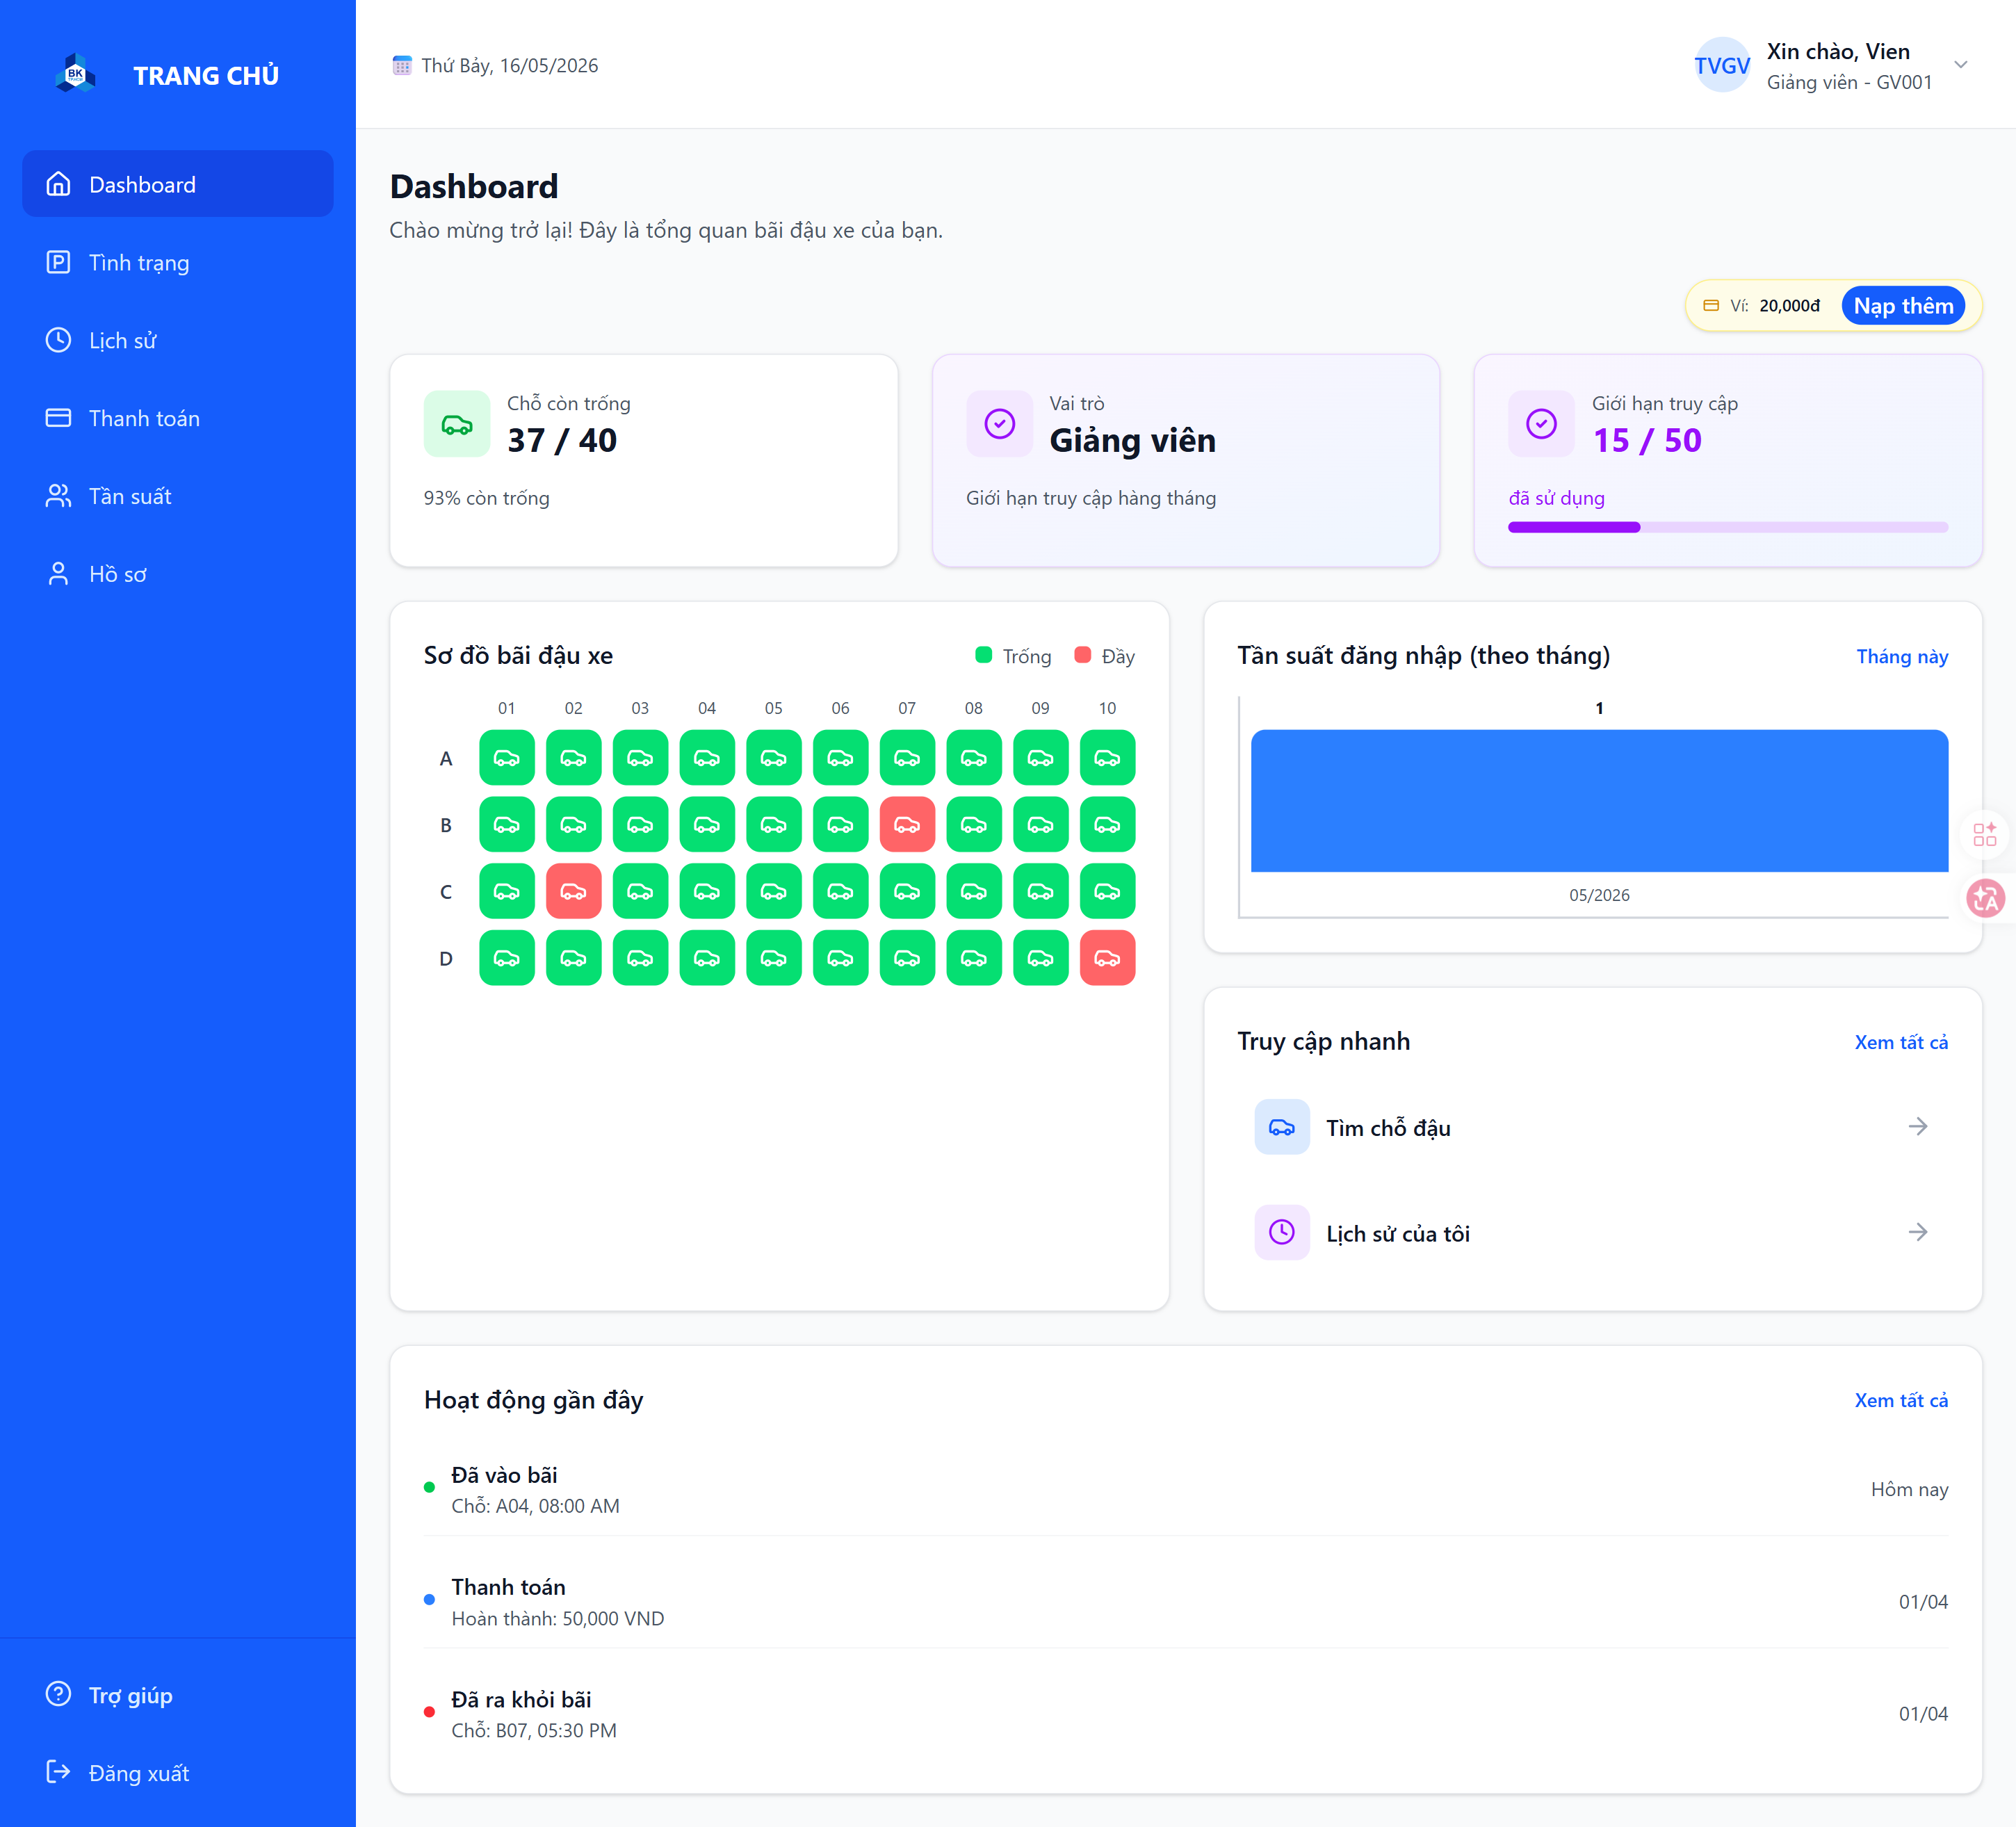
\includegraphics[width=1\linewidth]{Images/Task4/task4_lecturer_dashboard.png} 
	\caption{Dashboard dành cho giảng viên}
\end{figure}

\textbf{Bước 2.} Tại trang tần suất đăng nhập, giảng viên theo dõi biểu đồ số lượt ra vào theo tháng, lịch sử ra vào gần đây và mức sử dụng gói giới hạn truy cập.

\begin{figure}[H]
	\centering
	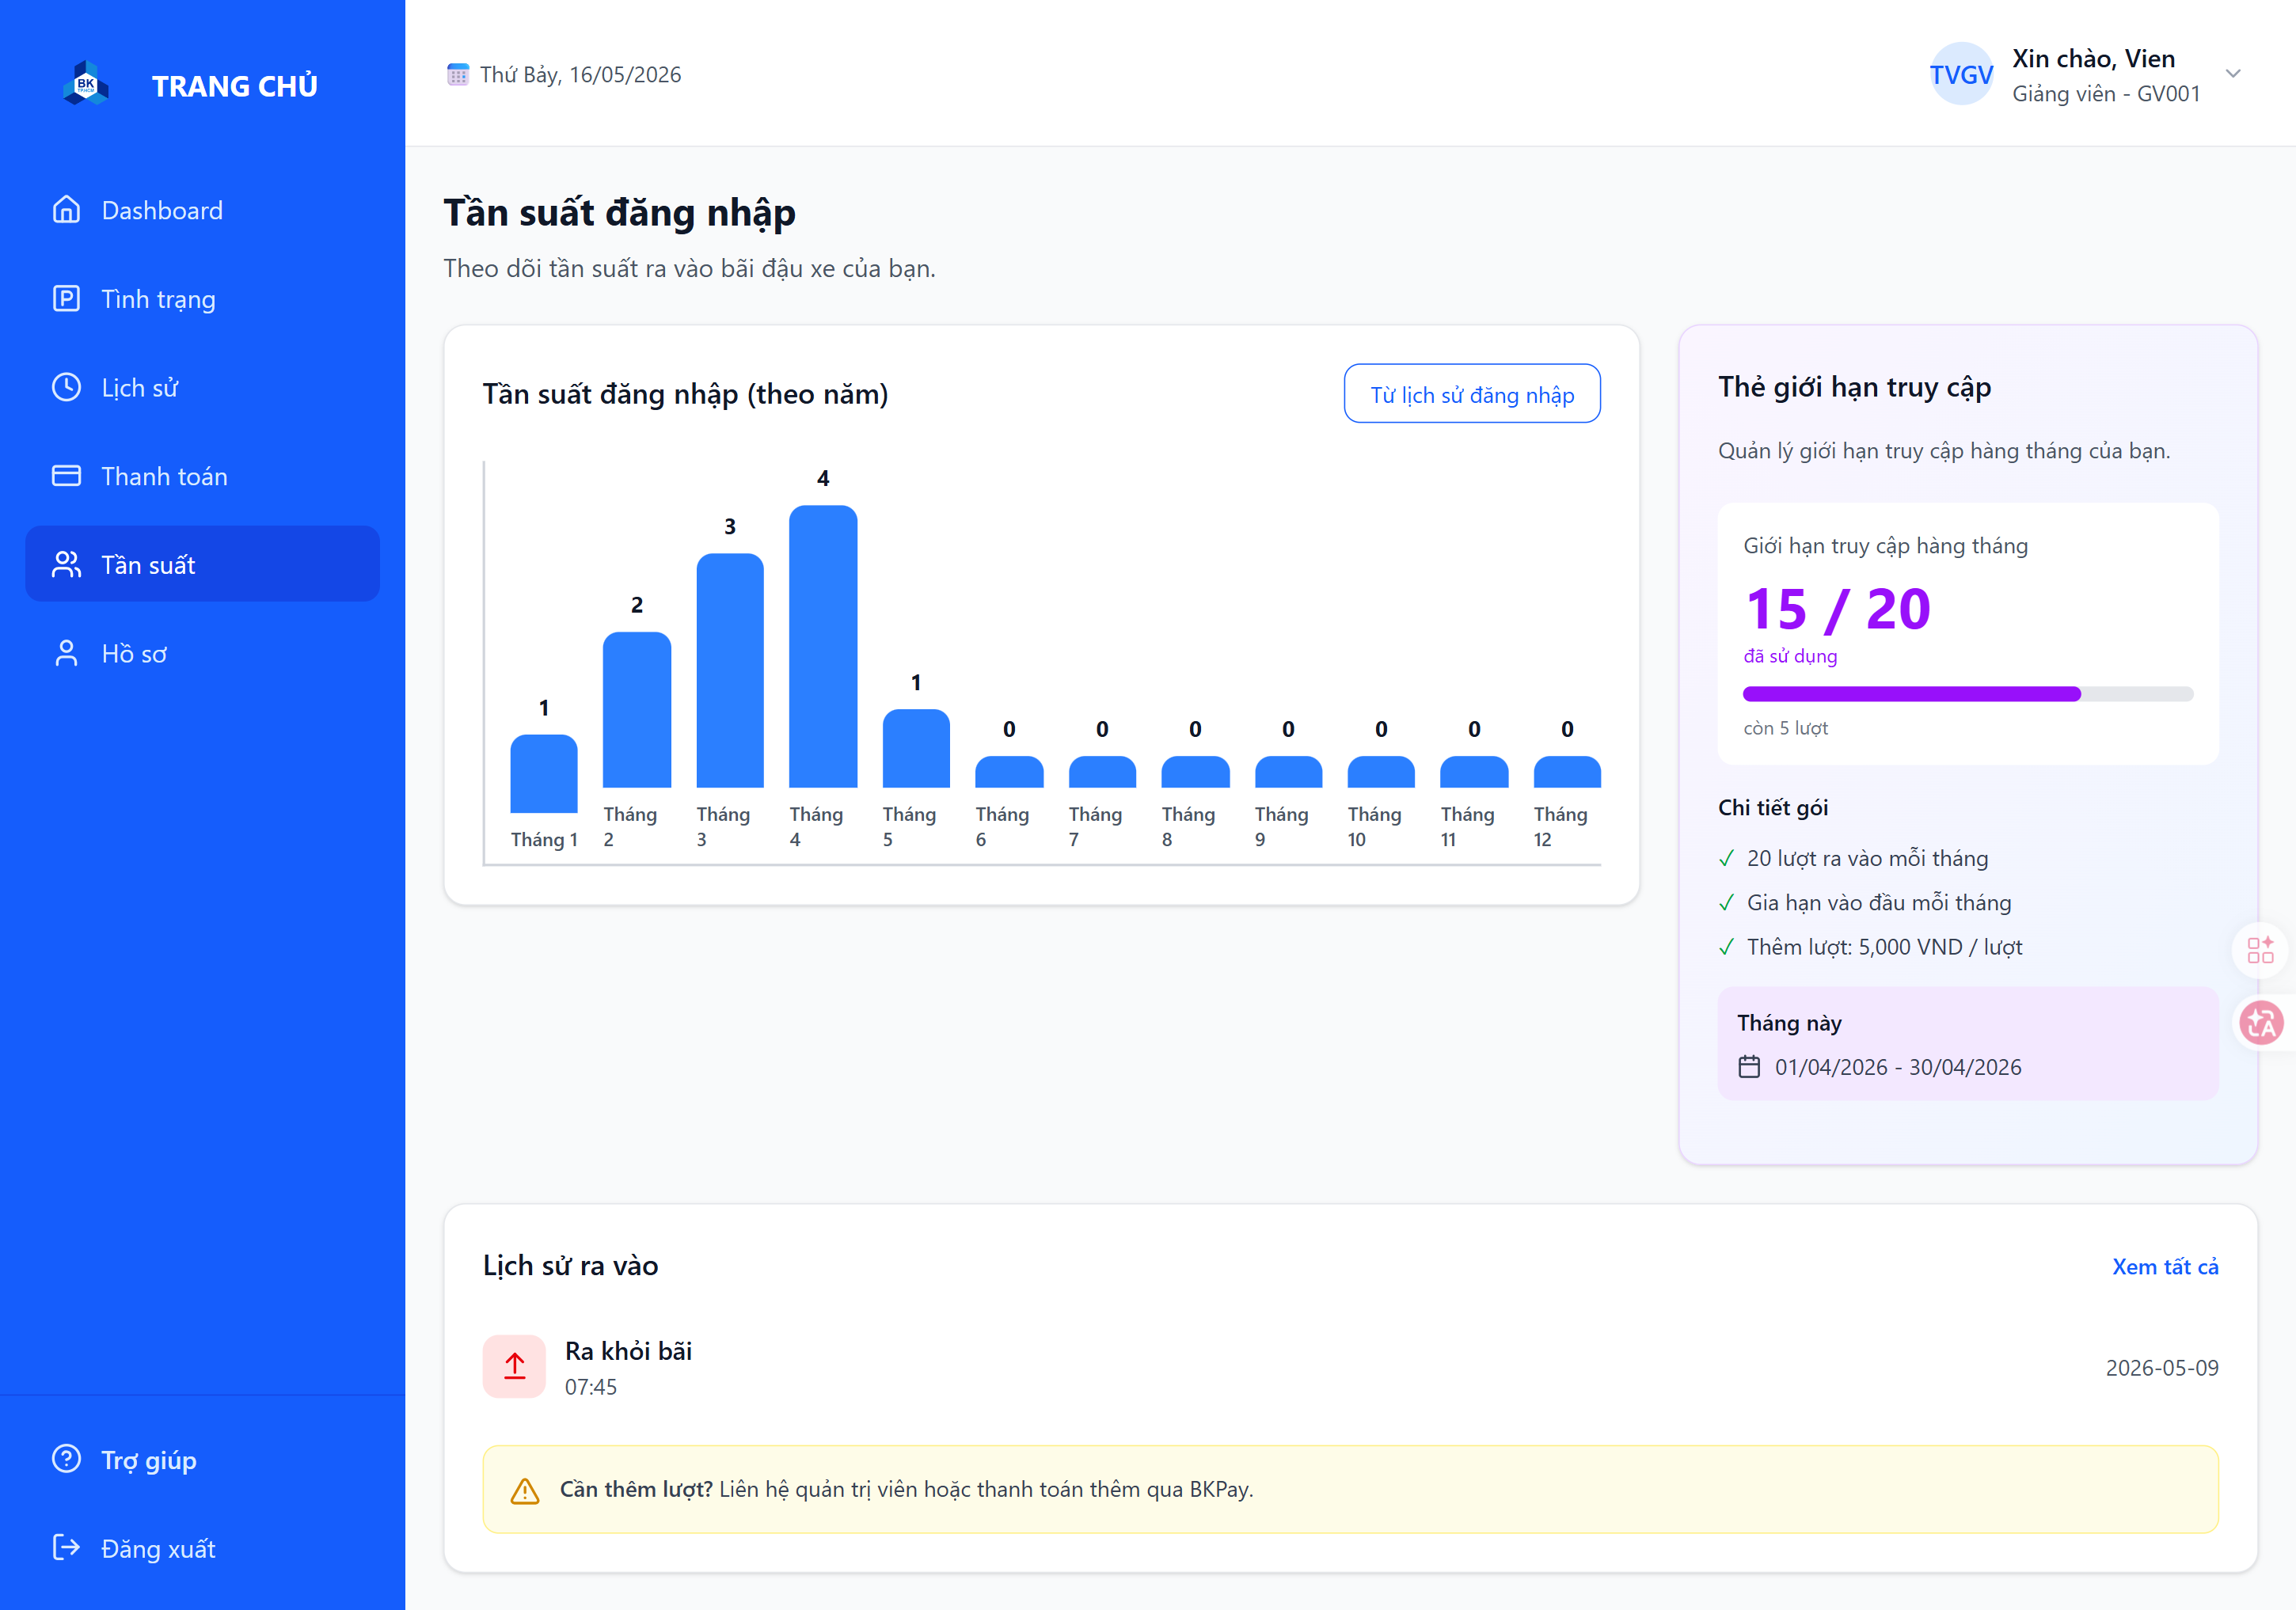
\includegraphics[width=1\linewidth]{Images/Task4/task4_lecturer_frequency.png} 
	\caption{Trang tần suất đăng nhập và giới hạn truy cập của giảng viên}
\end{figure}

\textbf{Bước 3.} Nếu cần thêm lượt vào bãi, giảng viên truy cập trang thanh toán, nhập số lượt cần mua và thực hiện thanh toán qua BKPay.

\begin{figure}[H]
	\centering
	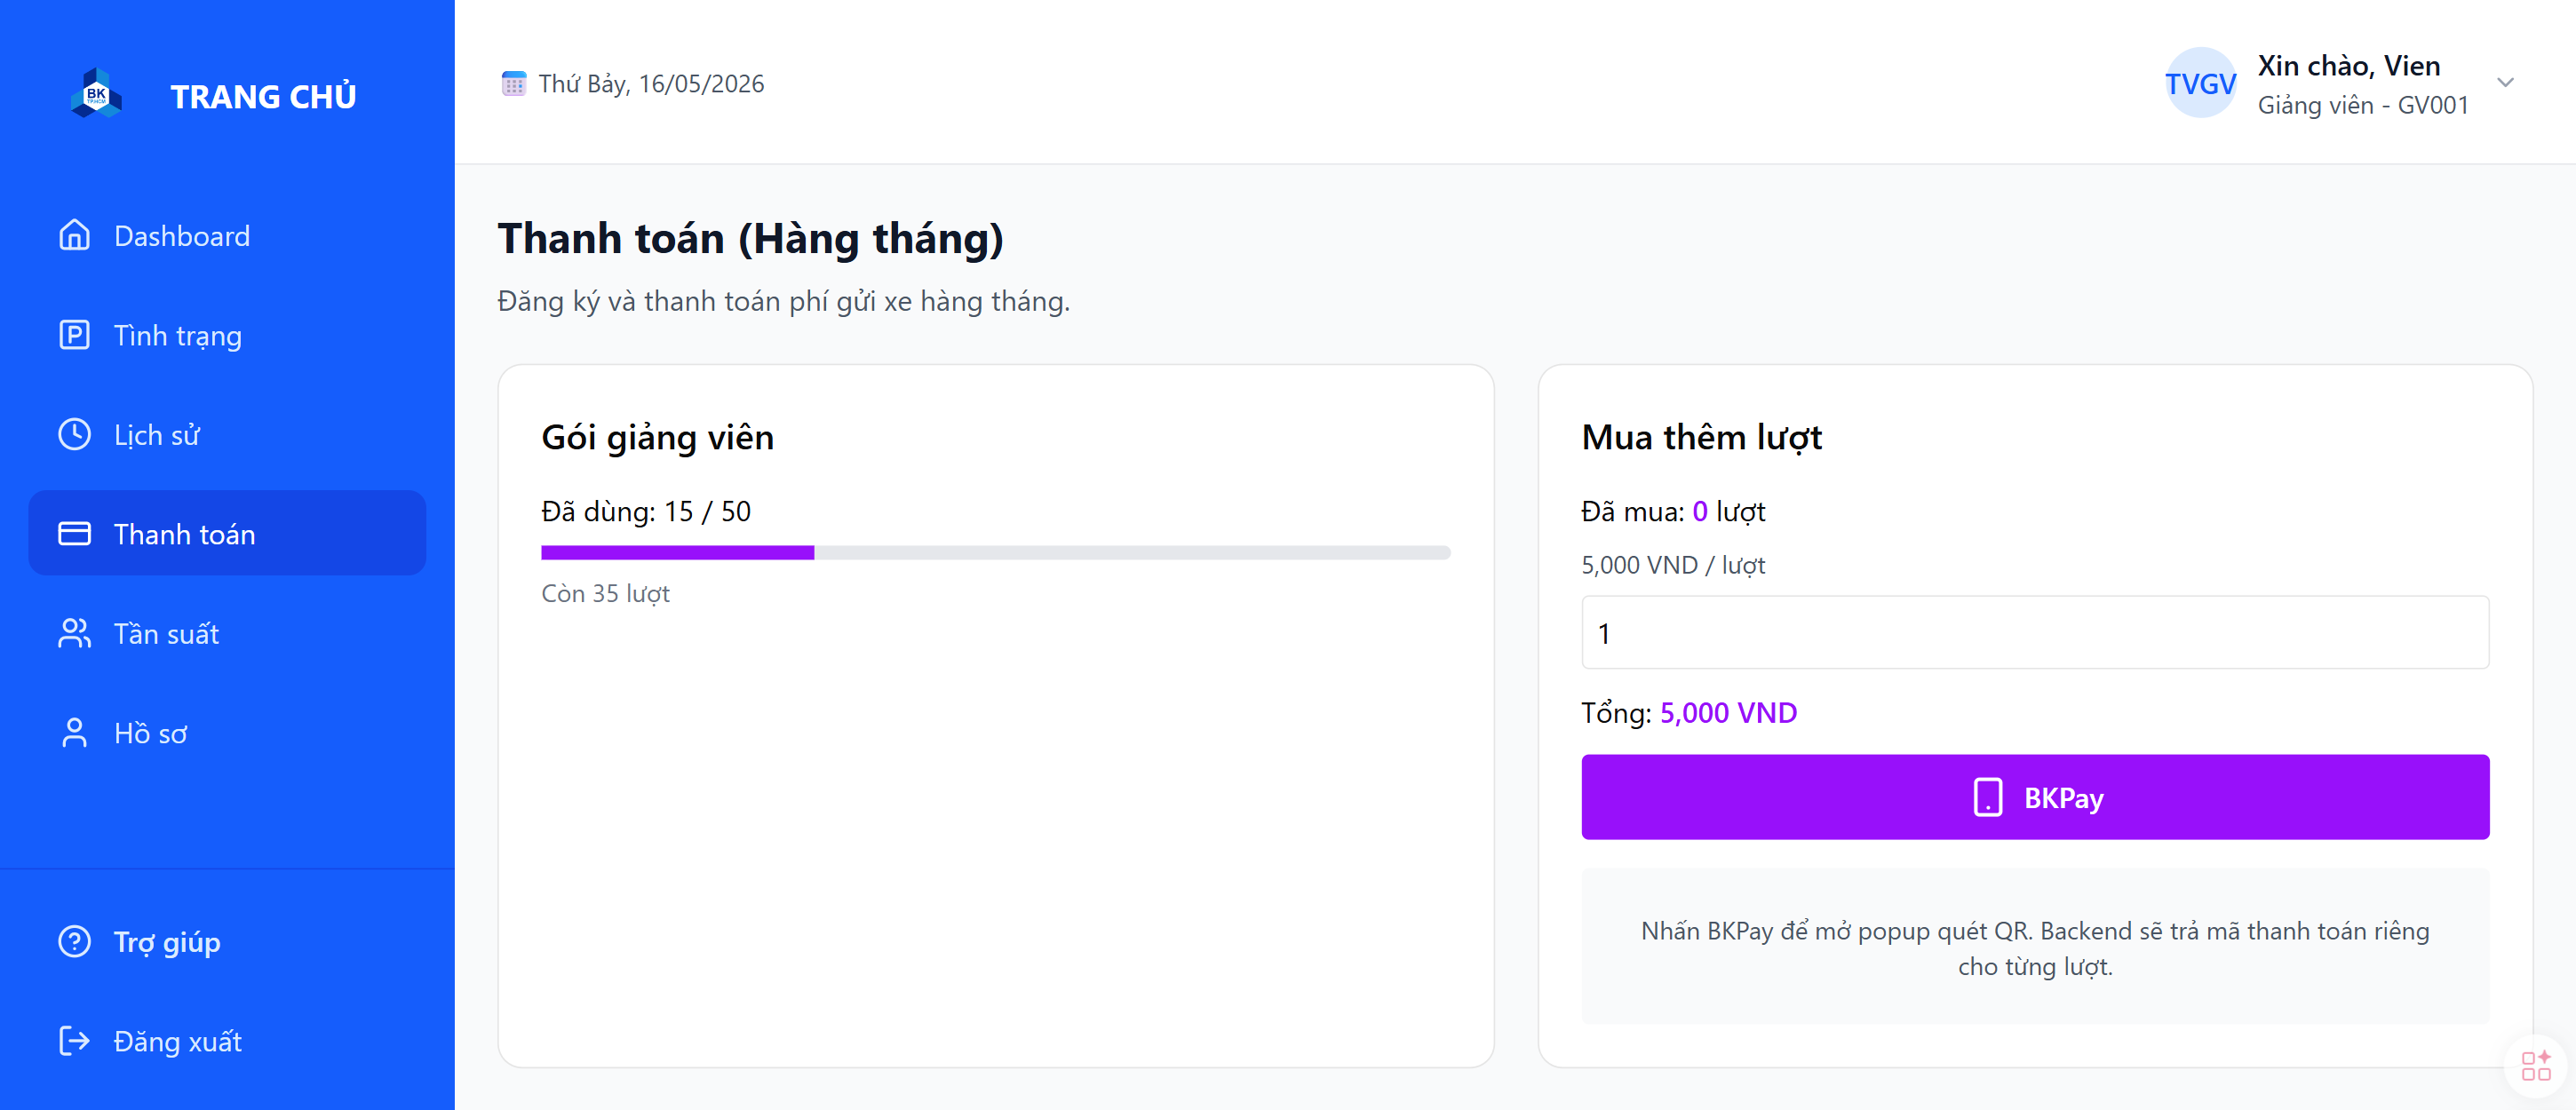
\includegraphics[width=1\linewidth]{Images/Task4/task4_lecturer_payment.png} 
	\caption{Trang mua thêm lượt gửi xe cho giảng viên}
\end{figure}

\textbf{Bước 4.} Sau khi chọn thanh toán, hệ thống tiếp tục hiển thị QR BKPay tương tự như luồng sinh viên nhưng áp dụng cho giao dịch mua thêm lượt sử dụng.

\begin{figure}[H]
	\centering
	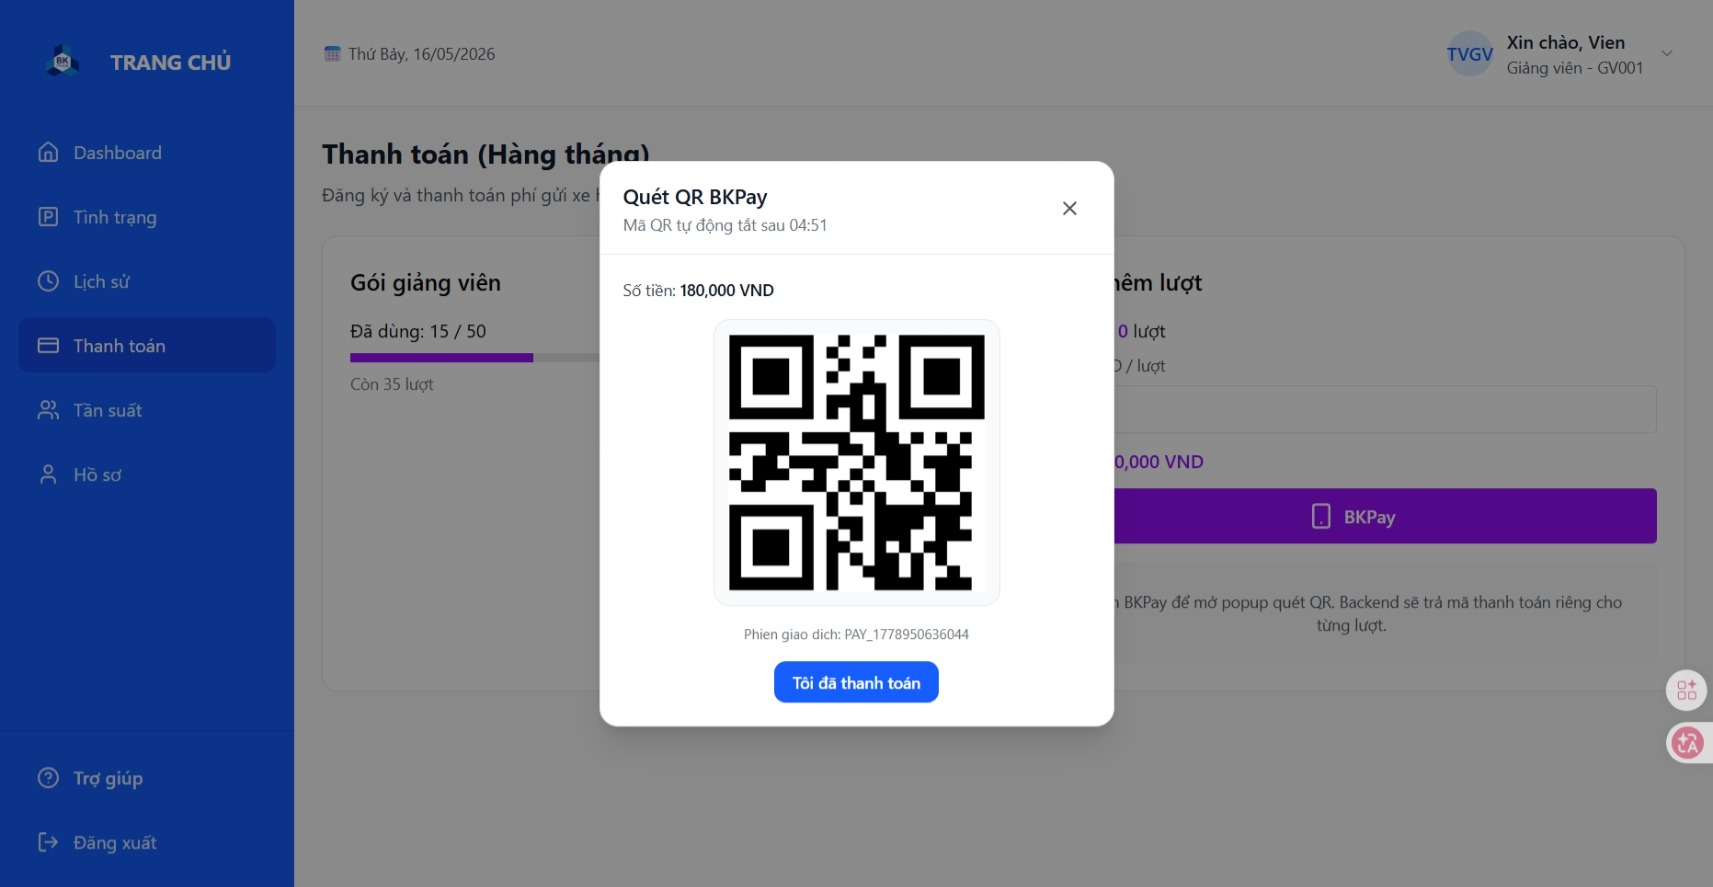
\includegraphics[width=1\linewidth]{Images/Task4/task4_lecturer_bkpay_qr.jpeg} 
	\caption{Popup QR BKPay cho giao dịch mua thêm lượt của giảng viên}
\end{figure}

\subsubsection{Chuỗi màn hình 6: Luồng nhân viên vận hành kiểm soát xe vãng lai}

\textbf{Bước 1.} Nhân viên đăng nhập bằng tài khoản vận hành để truy cập dashboard dành cho ca trực bãi xe.

\begin{figure}[H]
	\centering
	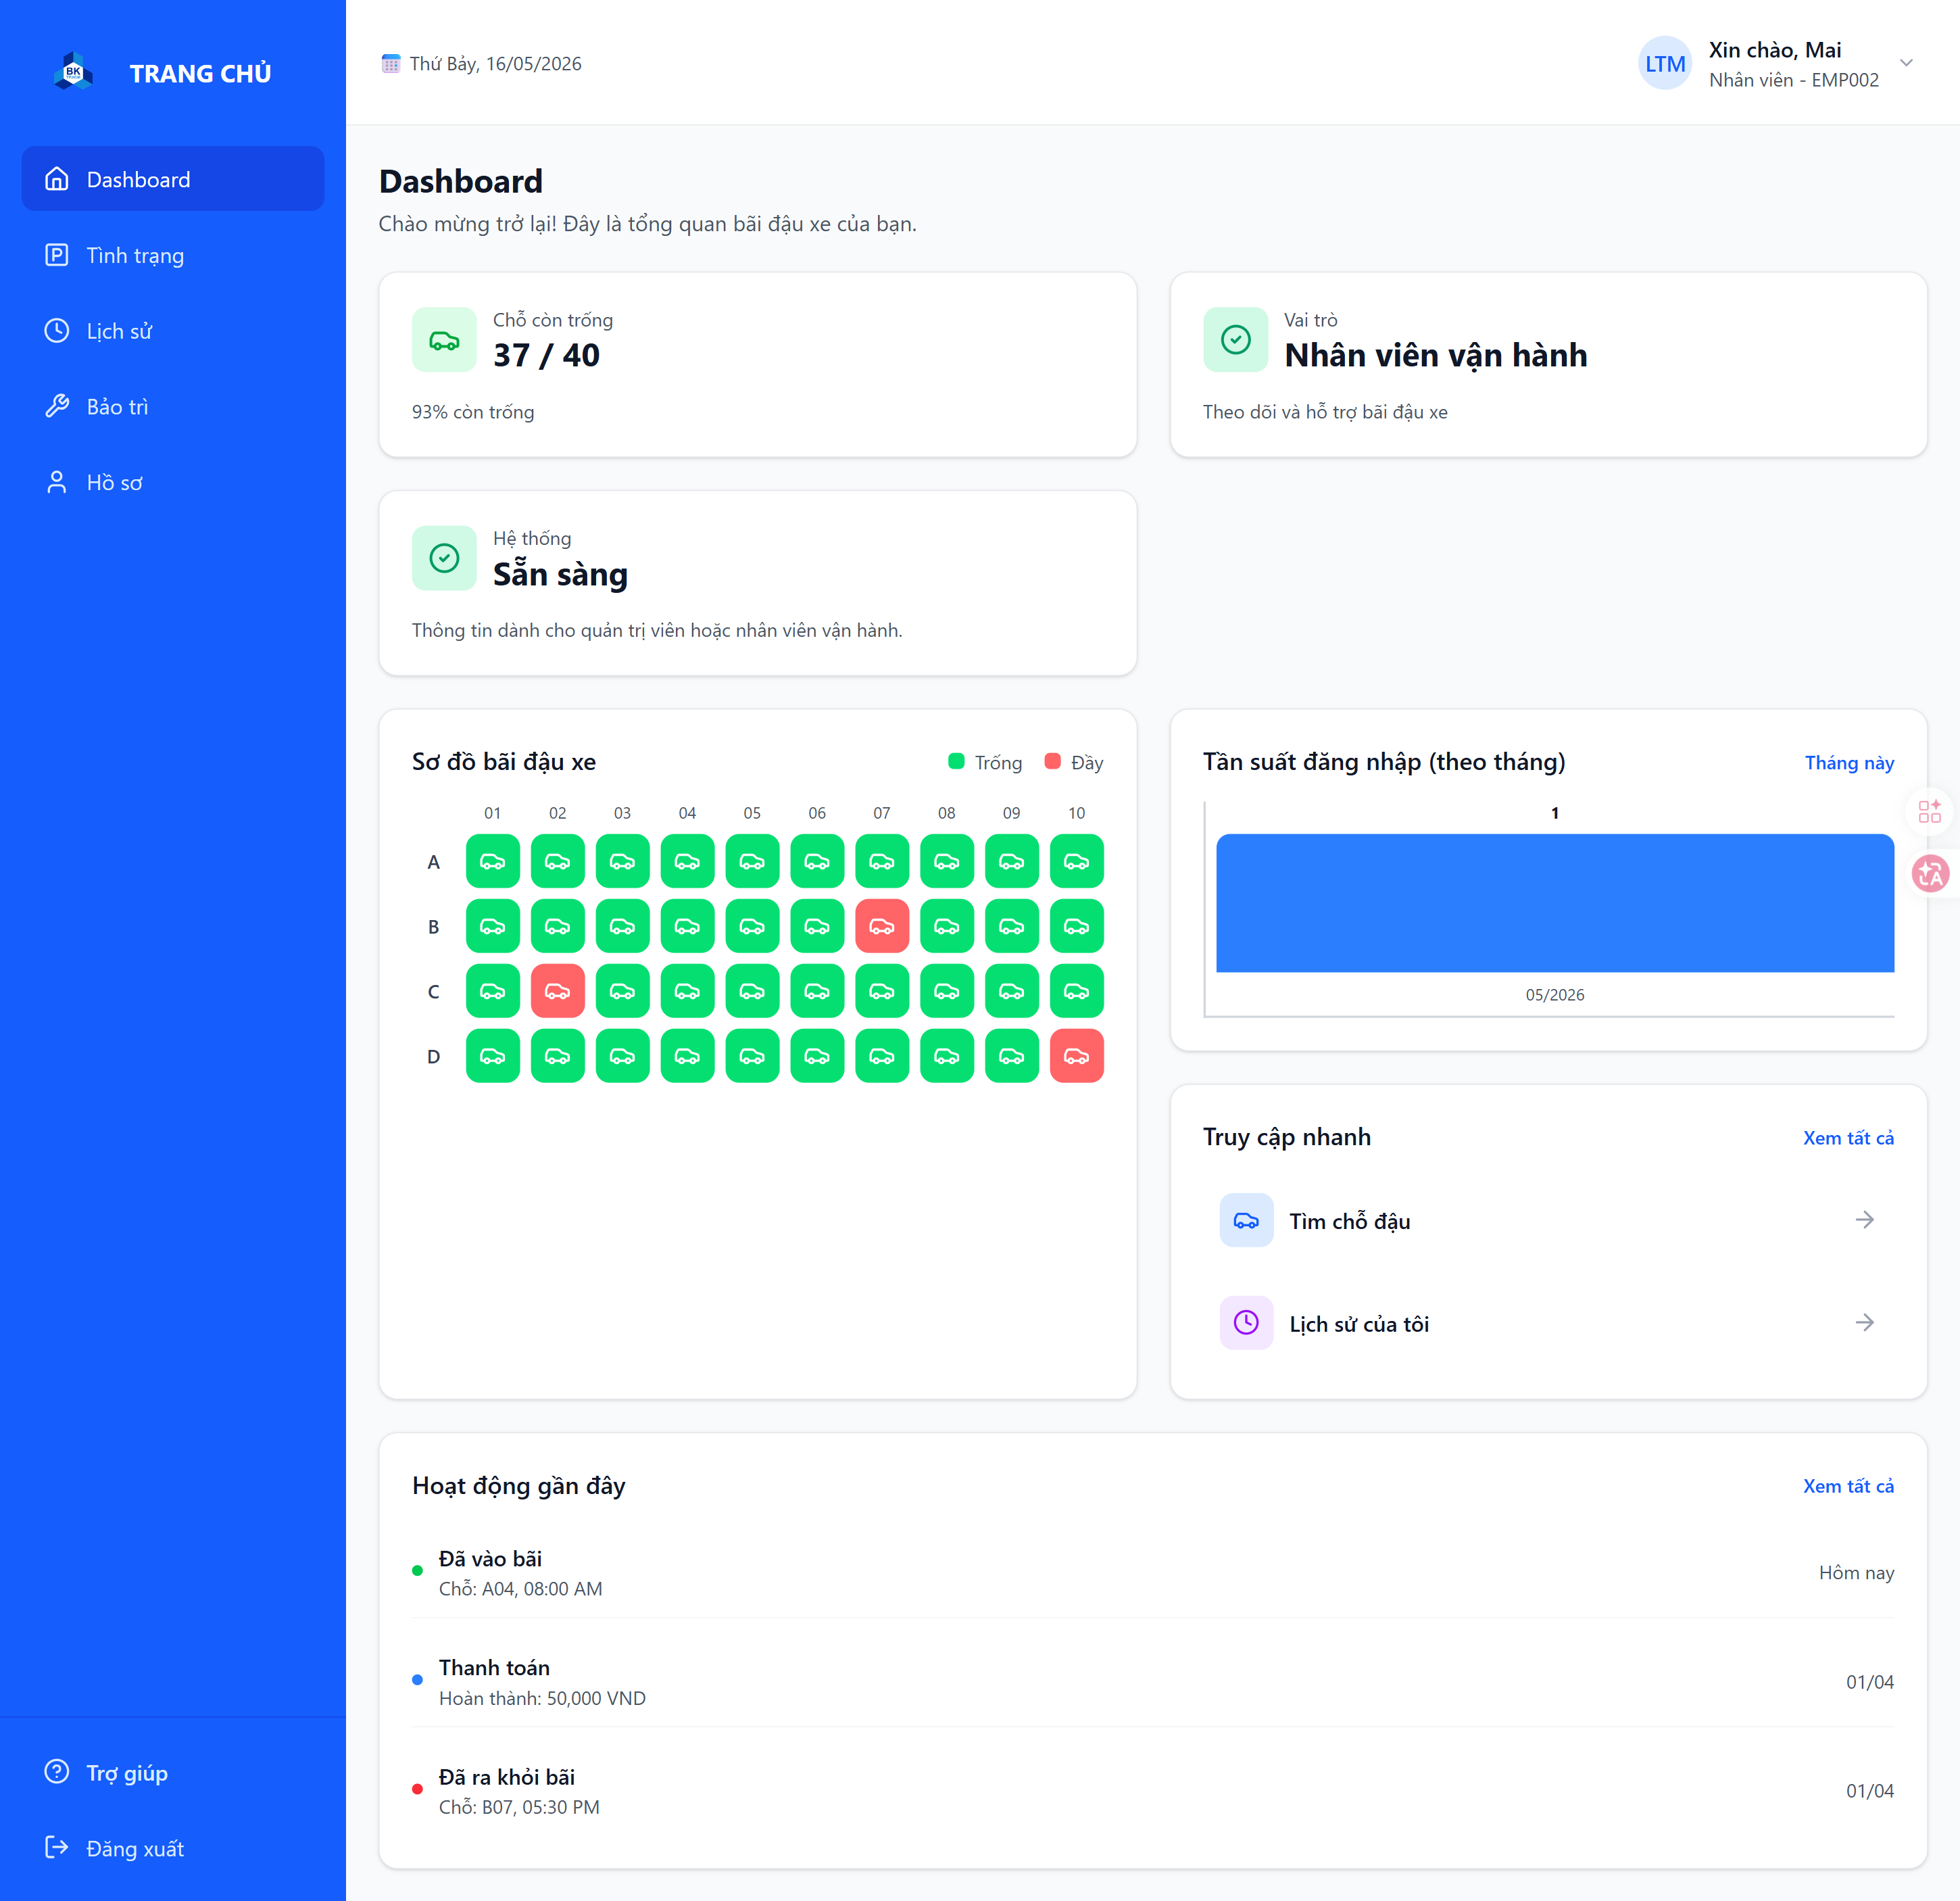
\includegraphics[width=1\linewidth]{Images/Task4/task4_employee_dashboard.png} 
	\caption{Dashboard dành cho nhân viên vận hành}
\end{figure}

\textbf{Bước 2.} Từ trang tình trạng bãi, nhân viên sử dụng khu vực mô phỏng quét khách để tạo phiên gửi xe tạm thời cho xe vãng lai. Màn hình thể hiện mã thẻ tạm, biển số, giờ vào và vị trí được gán.

\begin{figure}[H]
	\centering
	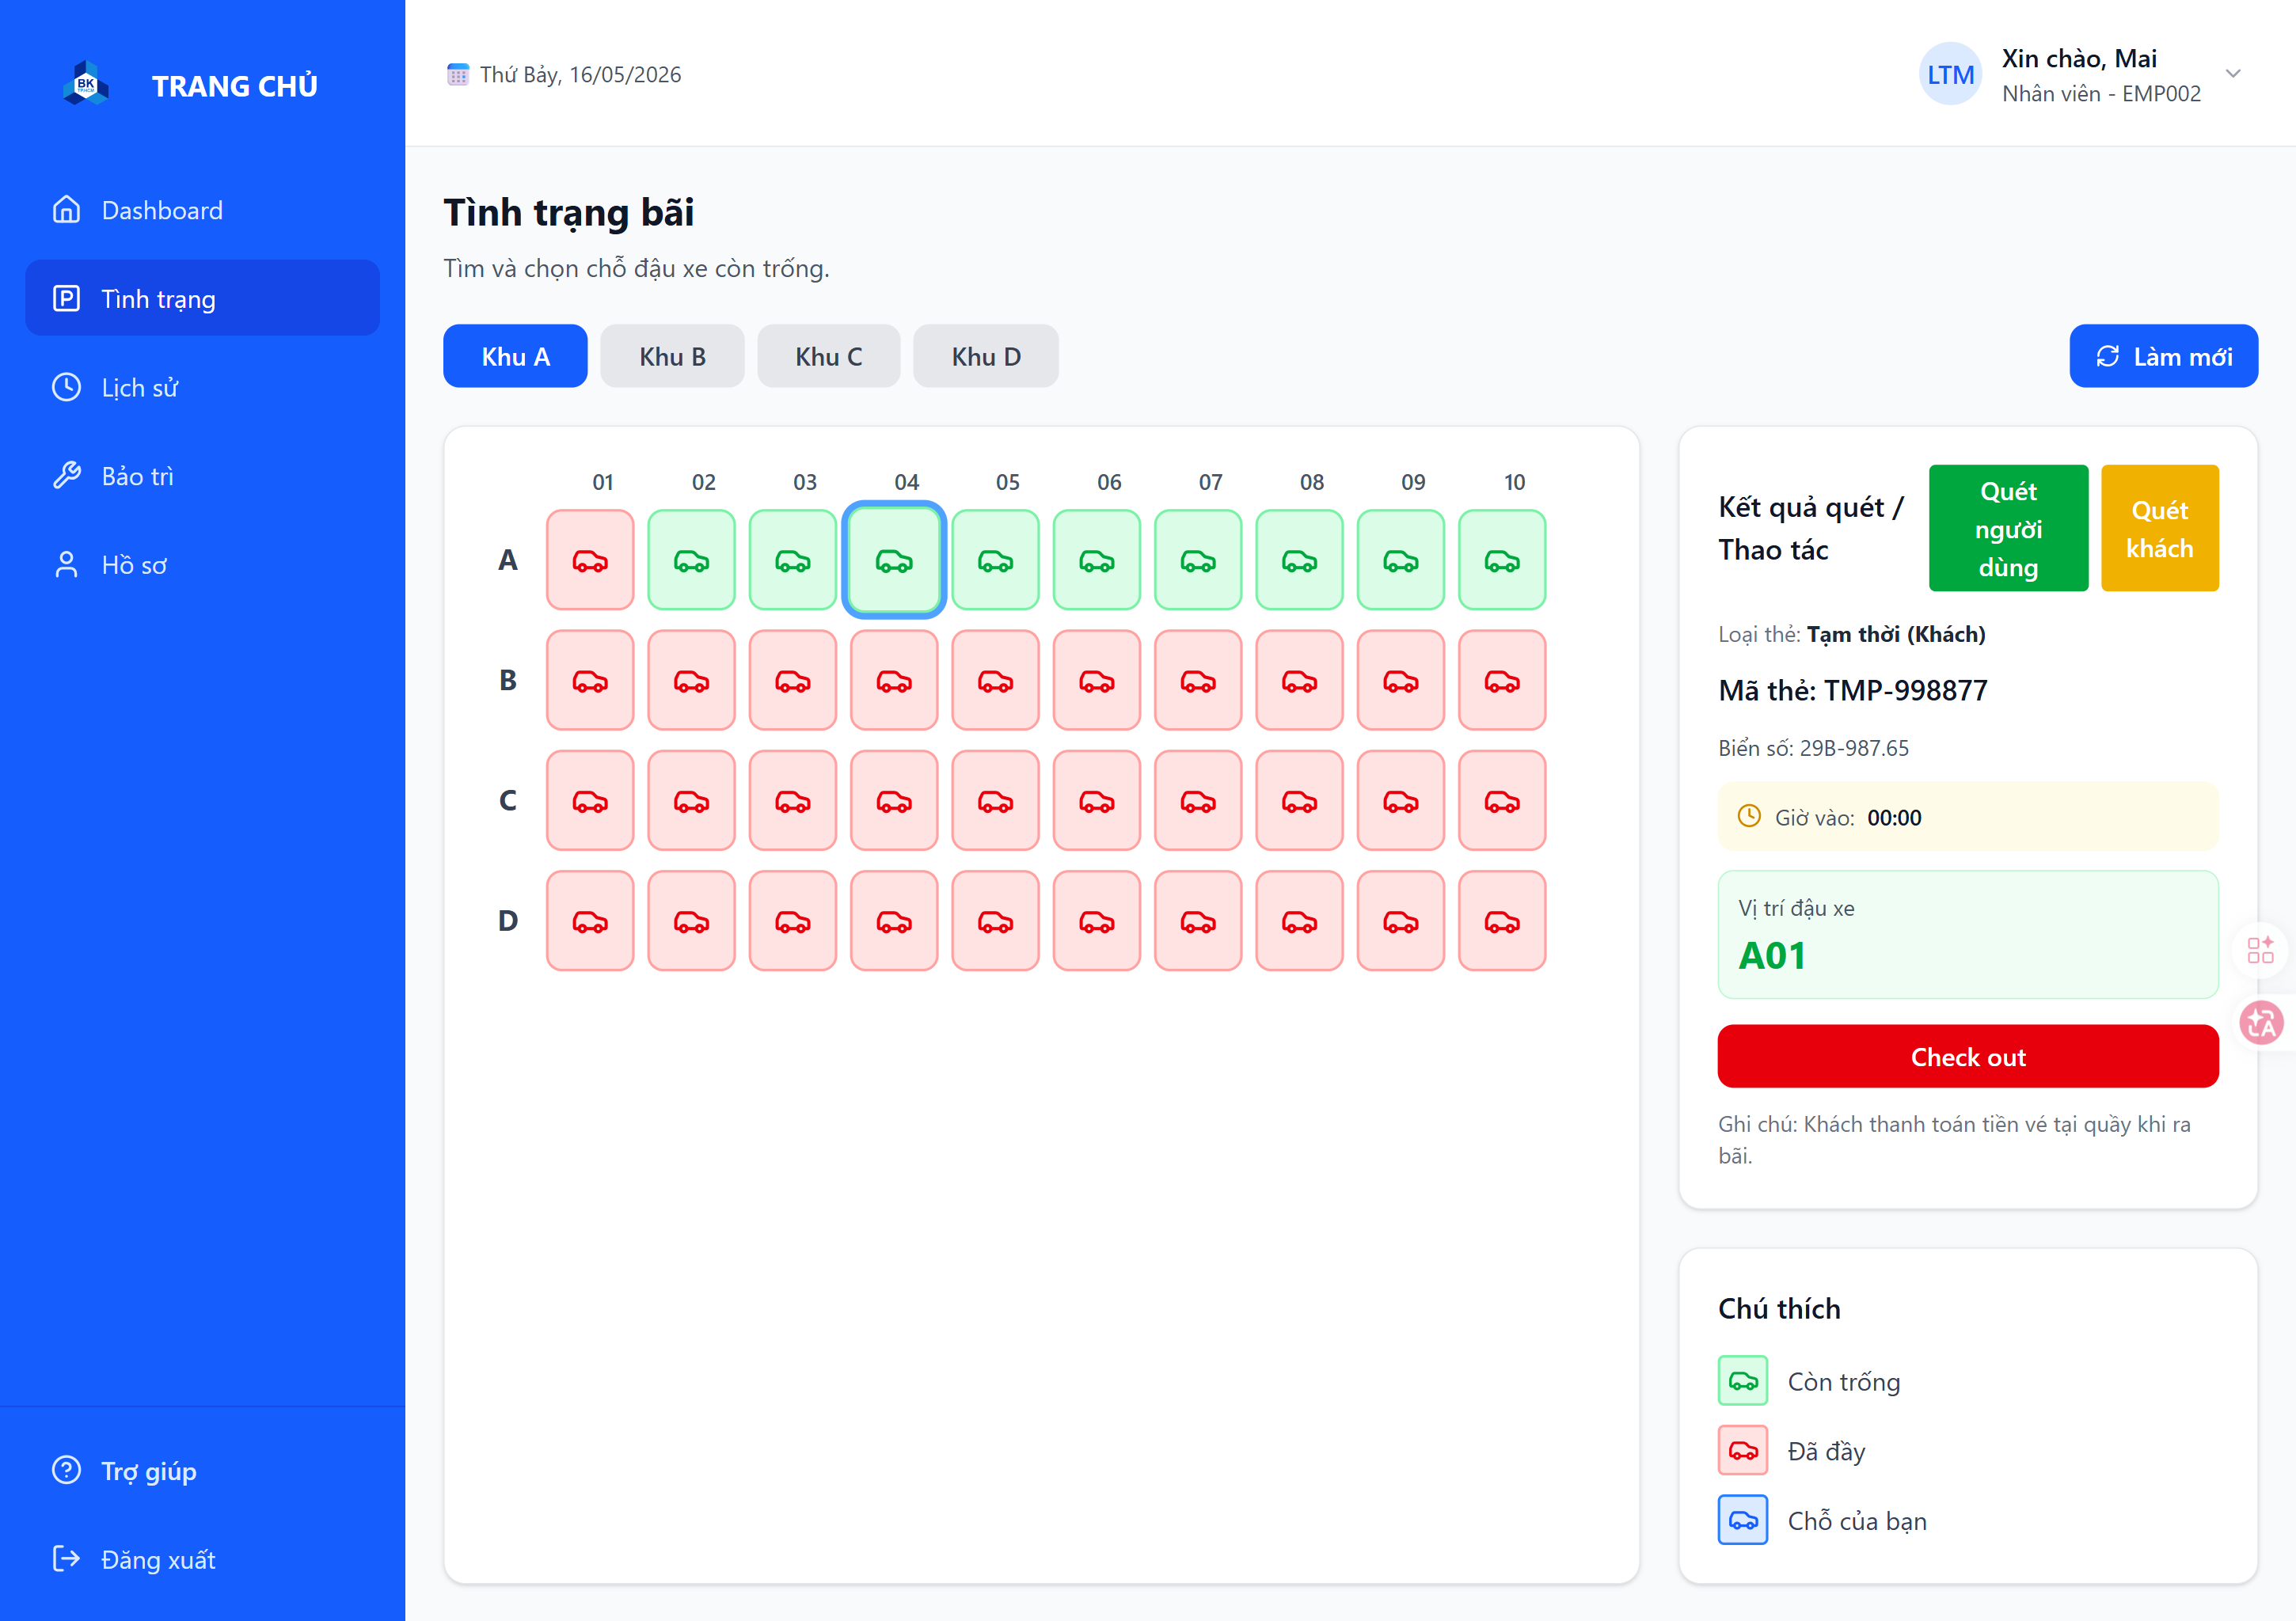
\includegraphics[width=1\linewidth]{Images/Task4/task4_employee_visitor_checkin.png} 
	\caption{Nhân viên tạo phiên gửi xe cho khách vãng lai}
\end{figure}

\textbf{Bước 3.} Khi khách ra bãi, nhân viên thao tác check-out. Màn hình minh họa phần thanh toán tại chỗ cho khách vãng lai và cập nhật kết thúc phiên gửi xe.

\begin{figure}[H]
	\centering
	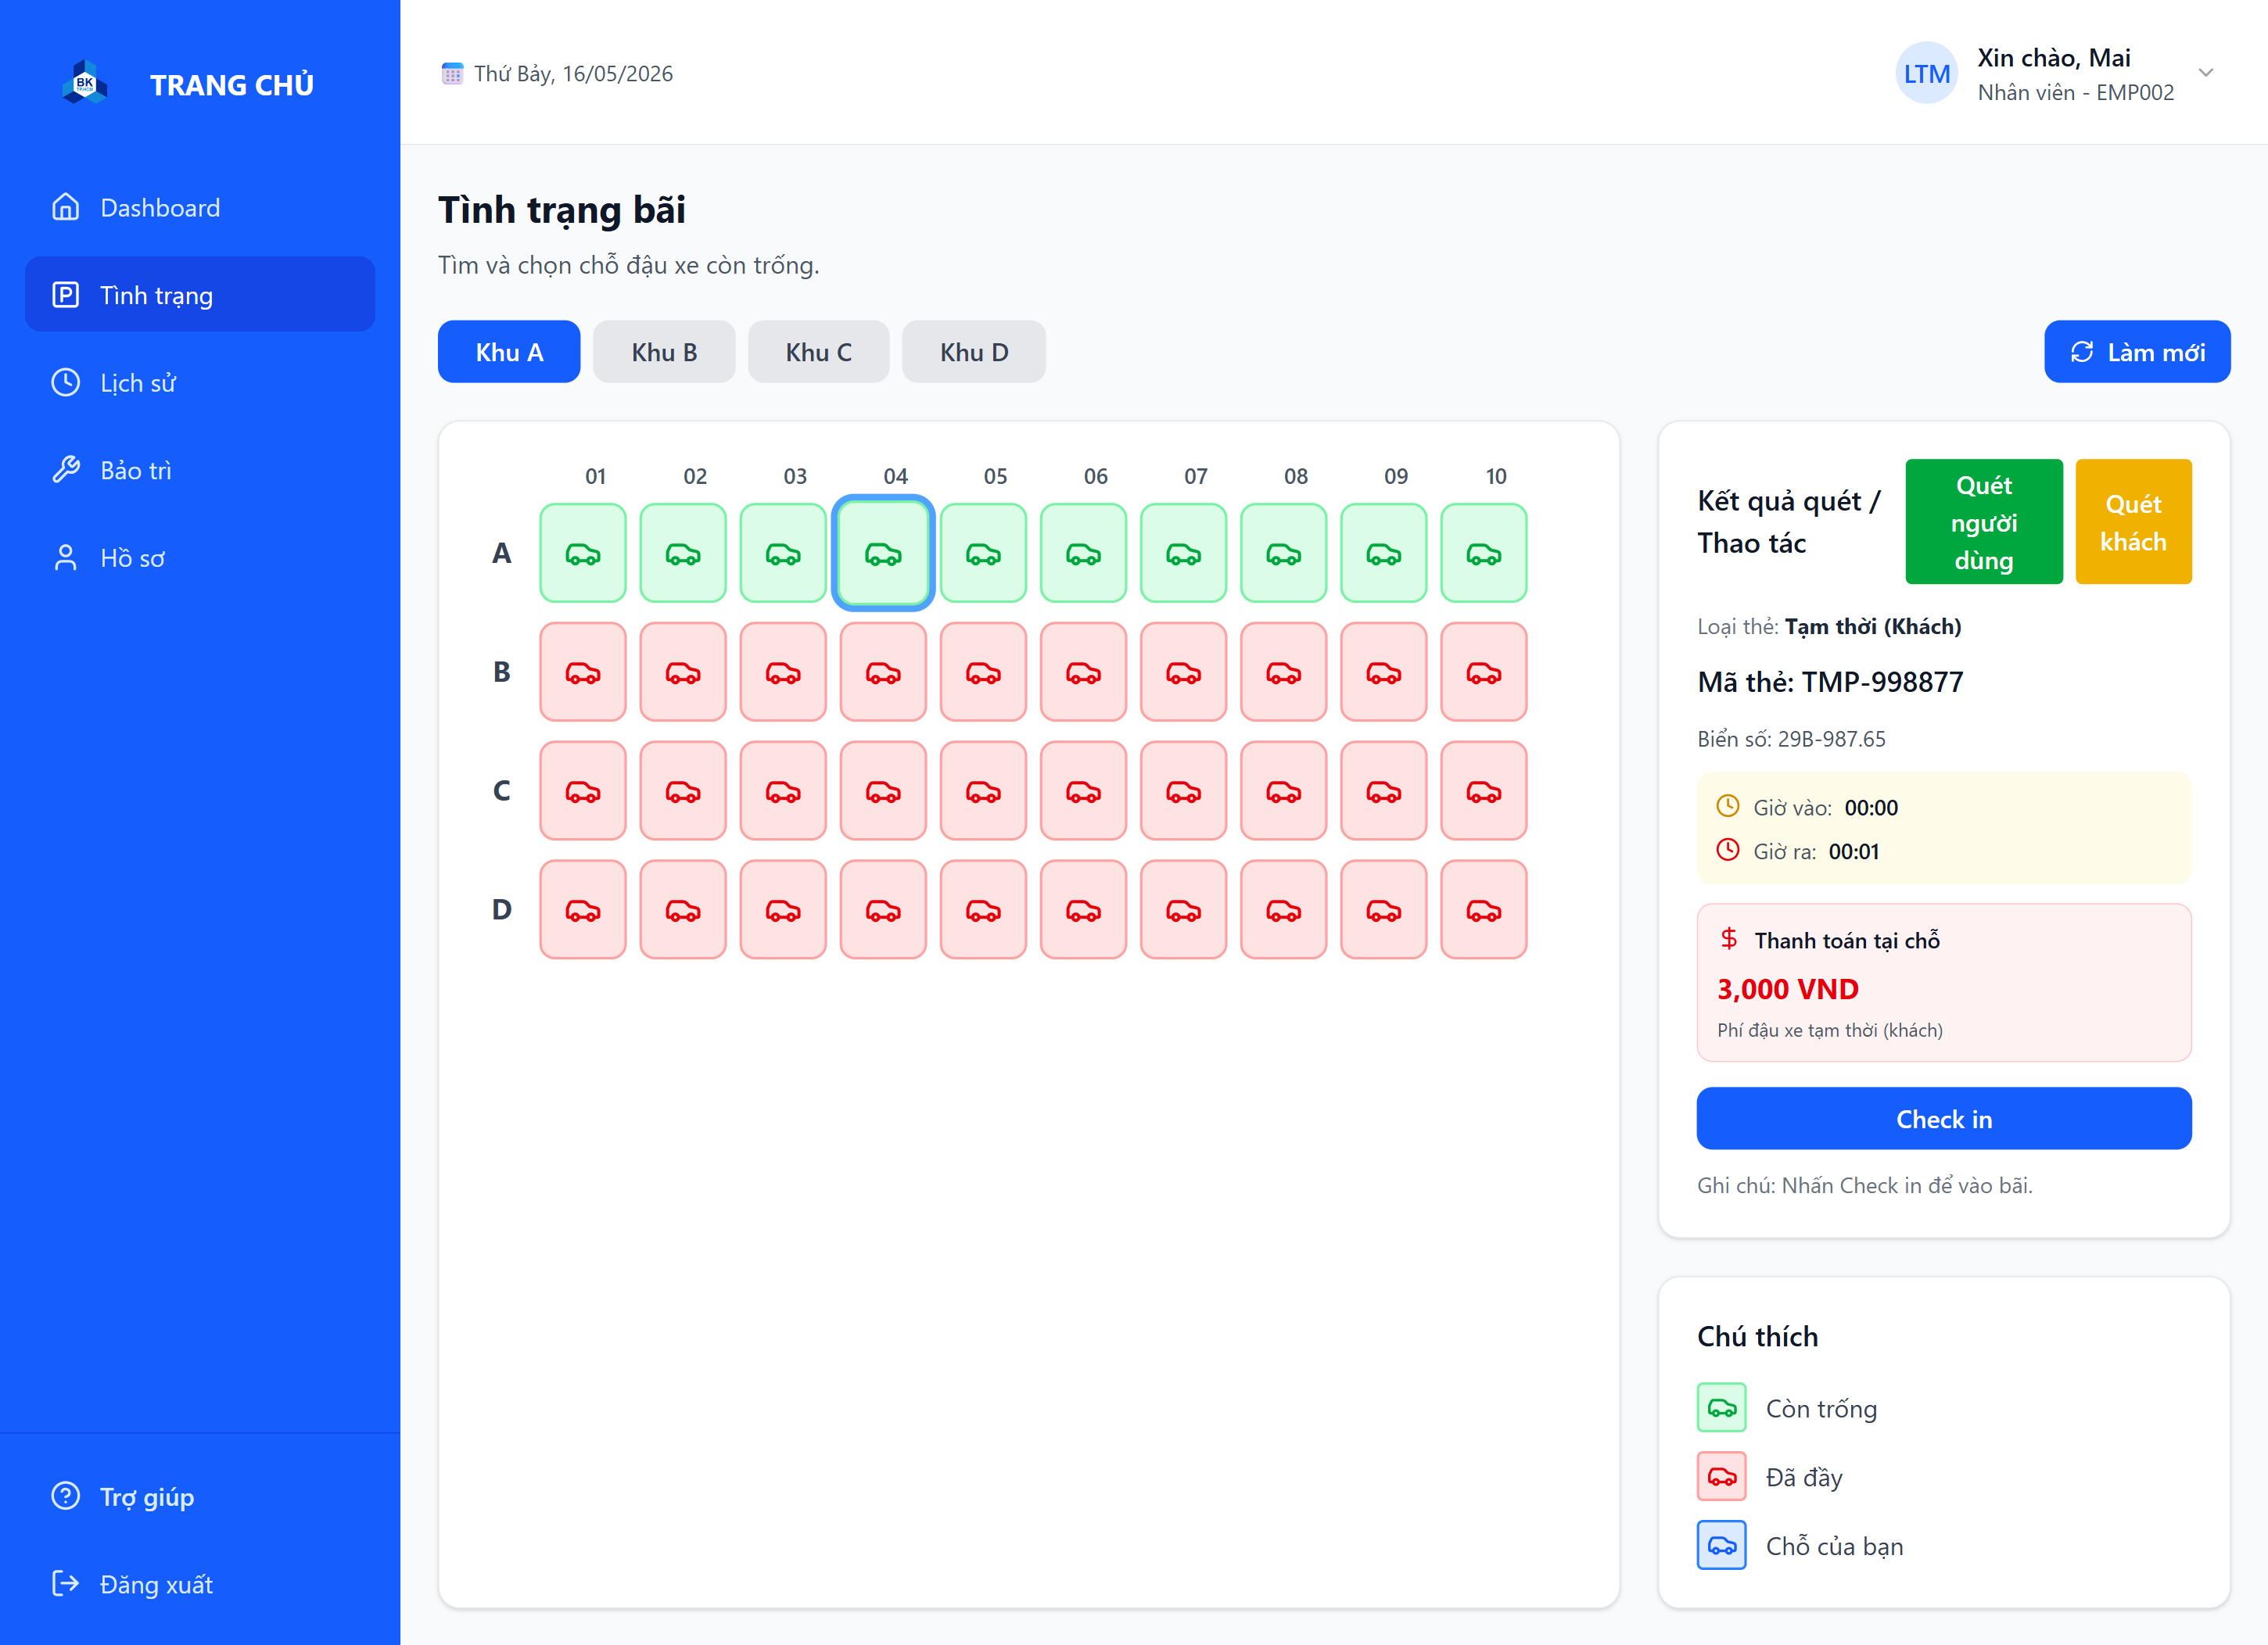
\includegraphics[width=1\linewidth]{Images/Task4/task4_employee_visitor_checkout.png} 
	\caption{Nhân viên xử lý check-out và thanh toán tại chỗ cho khách}
\end{figure}

\subsubsection{Chuỗi màn hình 7: Luồng nhân viên báo cáo và xử lý sự cố tại chỗ}

\textbf{Bước 1.} Nhân viên mở trang bảo trì để xem danh sách các sự cố hiện có, thống kê số lỗi theo trạng thái và bộ lọc theo khu vực, mức độ và từ khóa tìm kiếm.

\begin{figure}[H]
	\centering
	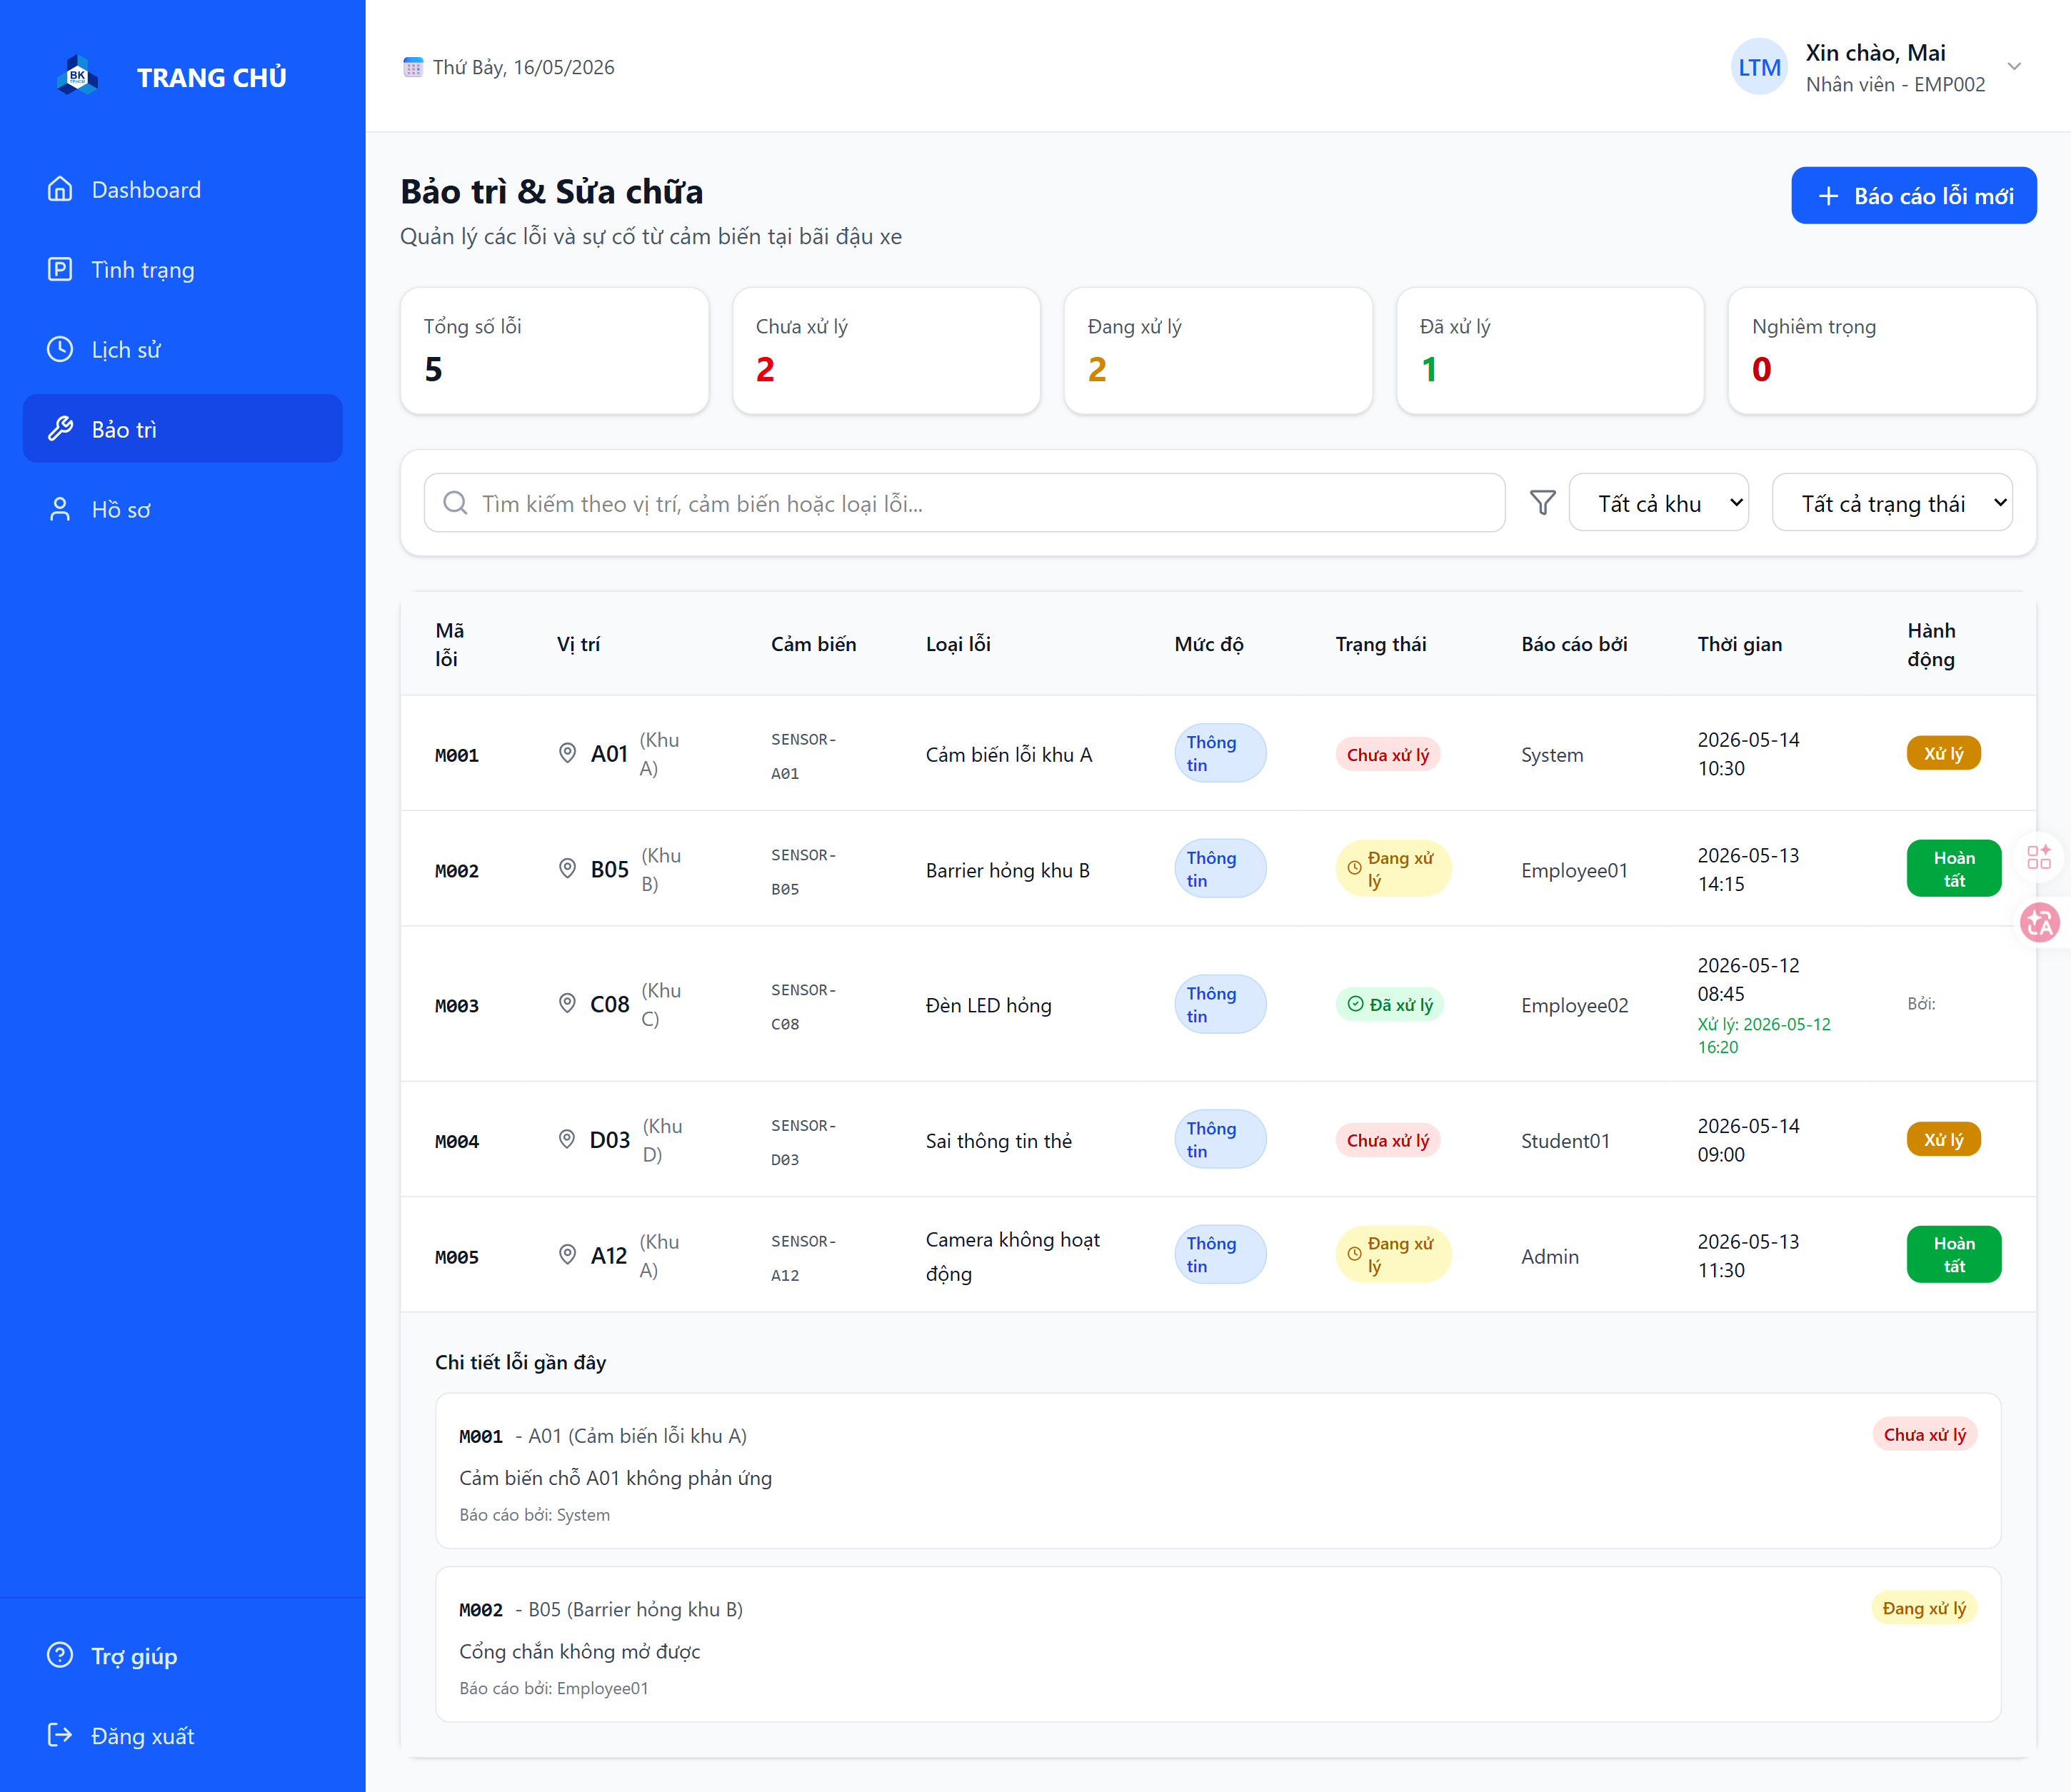
\includegraphics[width=1\linewidth]{Images/Task4/task4_employee_maintenance_list.png} 
	\caption{Trang bảo trì và danh sách sự cố của nhân viên}
\end{figure}

\textbf{Bước 2.} Khi phát hiện lỗi mới, nhân viên nhấn nút báo cáo lỗi mới. Hệ thống mở biểu mẫu để nhập loại sự cố, khu vực, vị trí, mức độ nghiêm trọng, mô tả chi tiết và tệp đính kèm.

\begin{figure}[H]
	\centering
	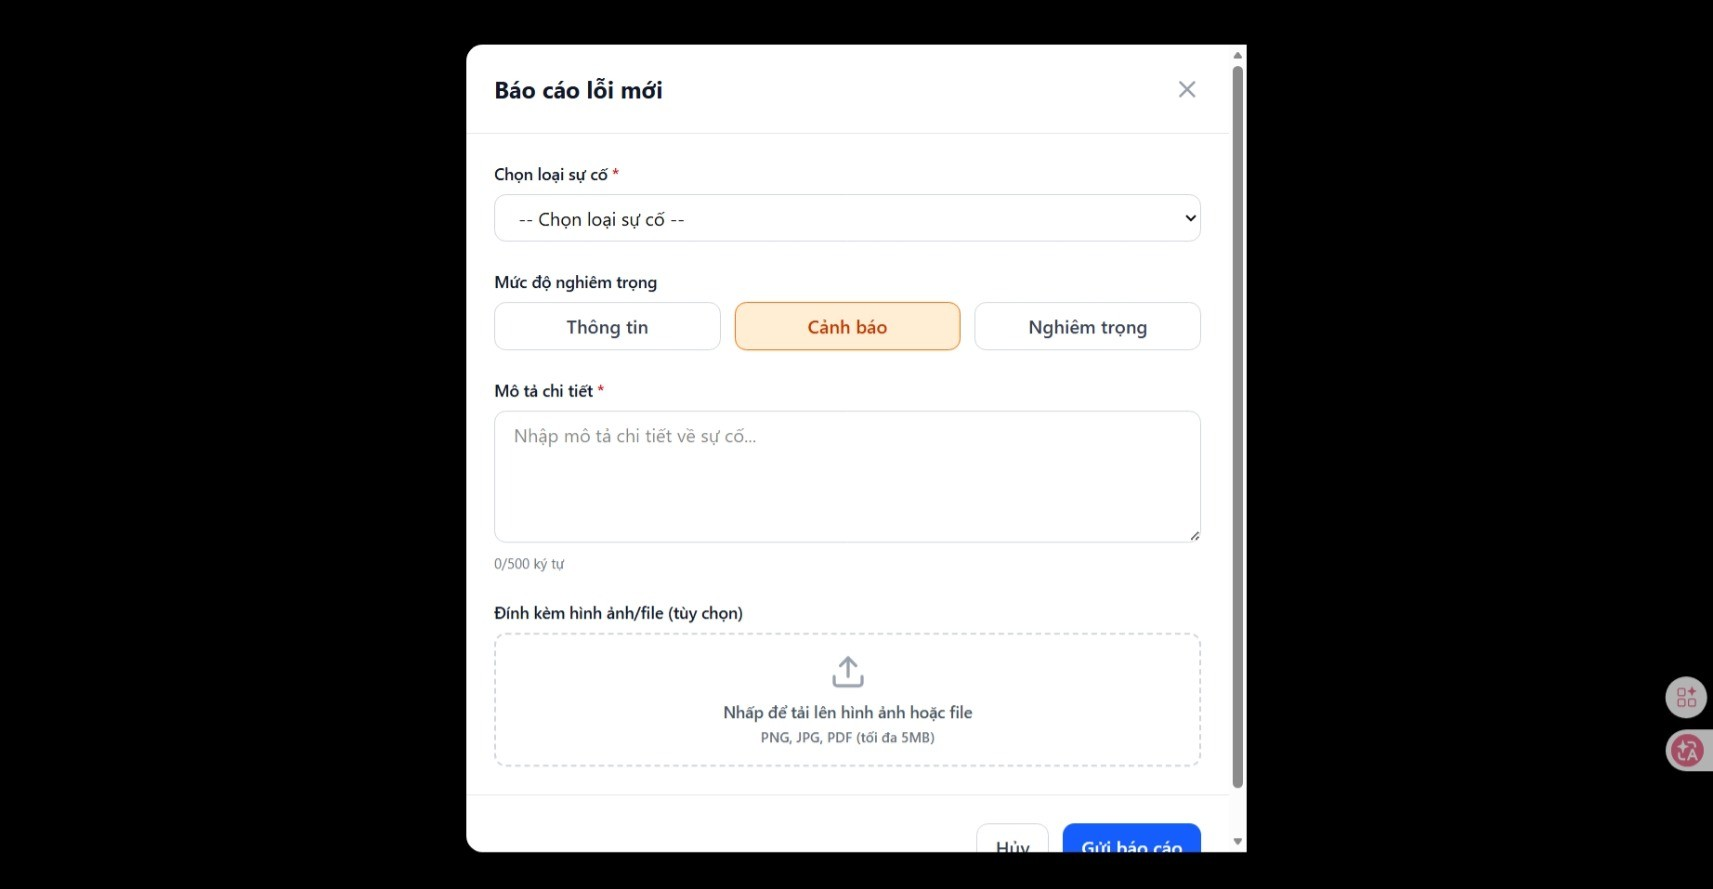
\includegraphics[width=1\linewidth]{Images/Task4/task4_employee_report_incident.jpeg} 
	\caption{Biểu mẫu báo cáo sự cố mới của nhân viên}
\end{figure}

\textbf{Bước 3.} Sau khi gửi, hệ thống thêm bản ghi sự cố vào danh sách để phục vụ theo dõi và cập nhật trạng thái xử lý.

\begin{figure}[H]
	\centering
	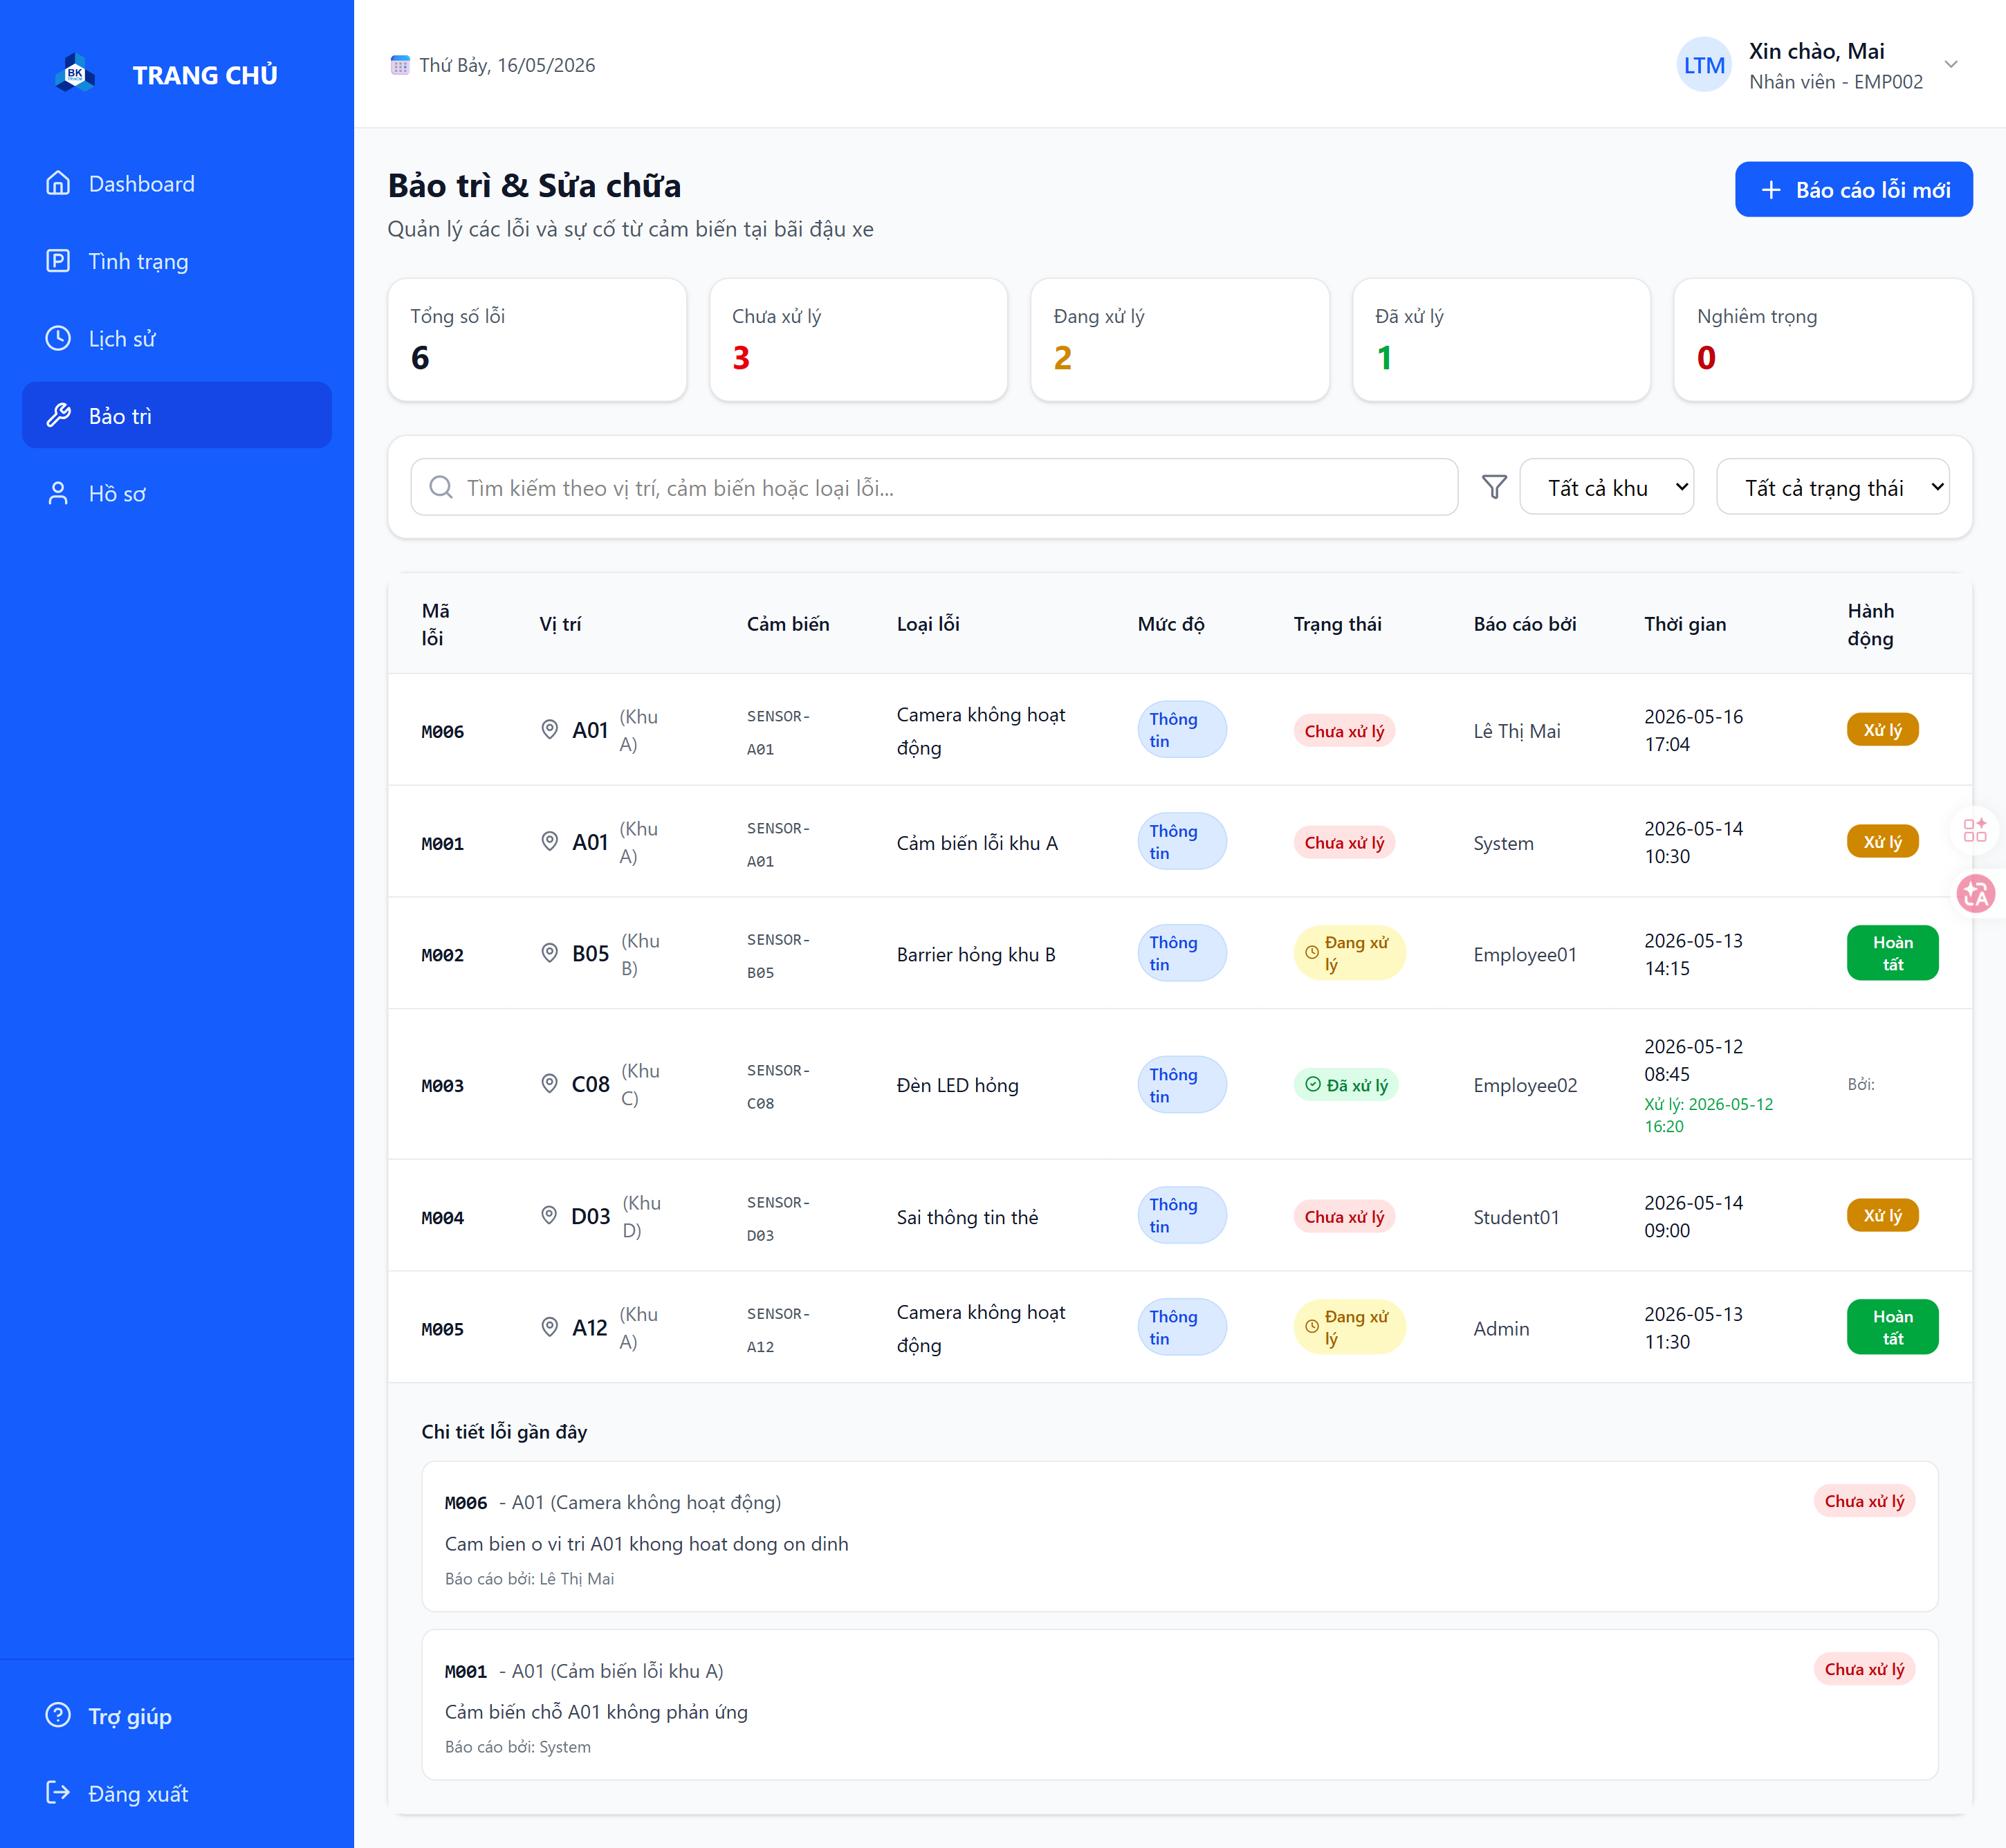
\includegraphics[width=1\linewidth]{Images/Task4/task4_employee_incident_submitted.png} 
	\caption{Danh sách sự cố sau khi nhân viên gửi báo cáo}
\end{figure}

\subsubsection{Chuỗi màn hình 8: Luồng quản trị viên theo dõi vận hành hệ thống}

\textbf{Bước 1.} Quản trị viên đăng nhập bằng tài khoản quản trị và được chuyển đến dashboard tổng quan. Màn hình hiển thị số chỗ trống, vai trò quản trị viên, sơ đồ bãi xe và tần suất truy cập.

\begin{figure}[H]
	\centering
	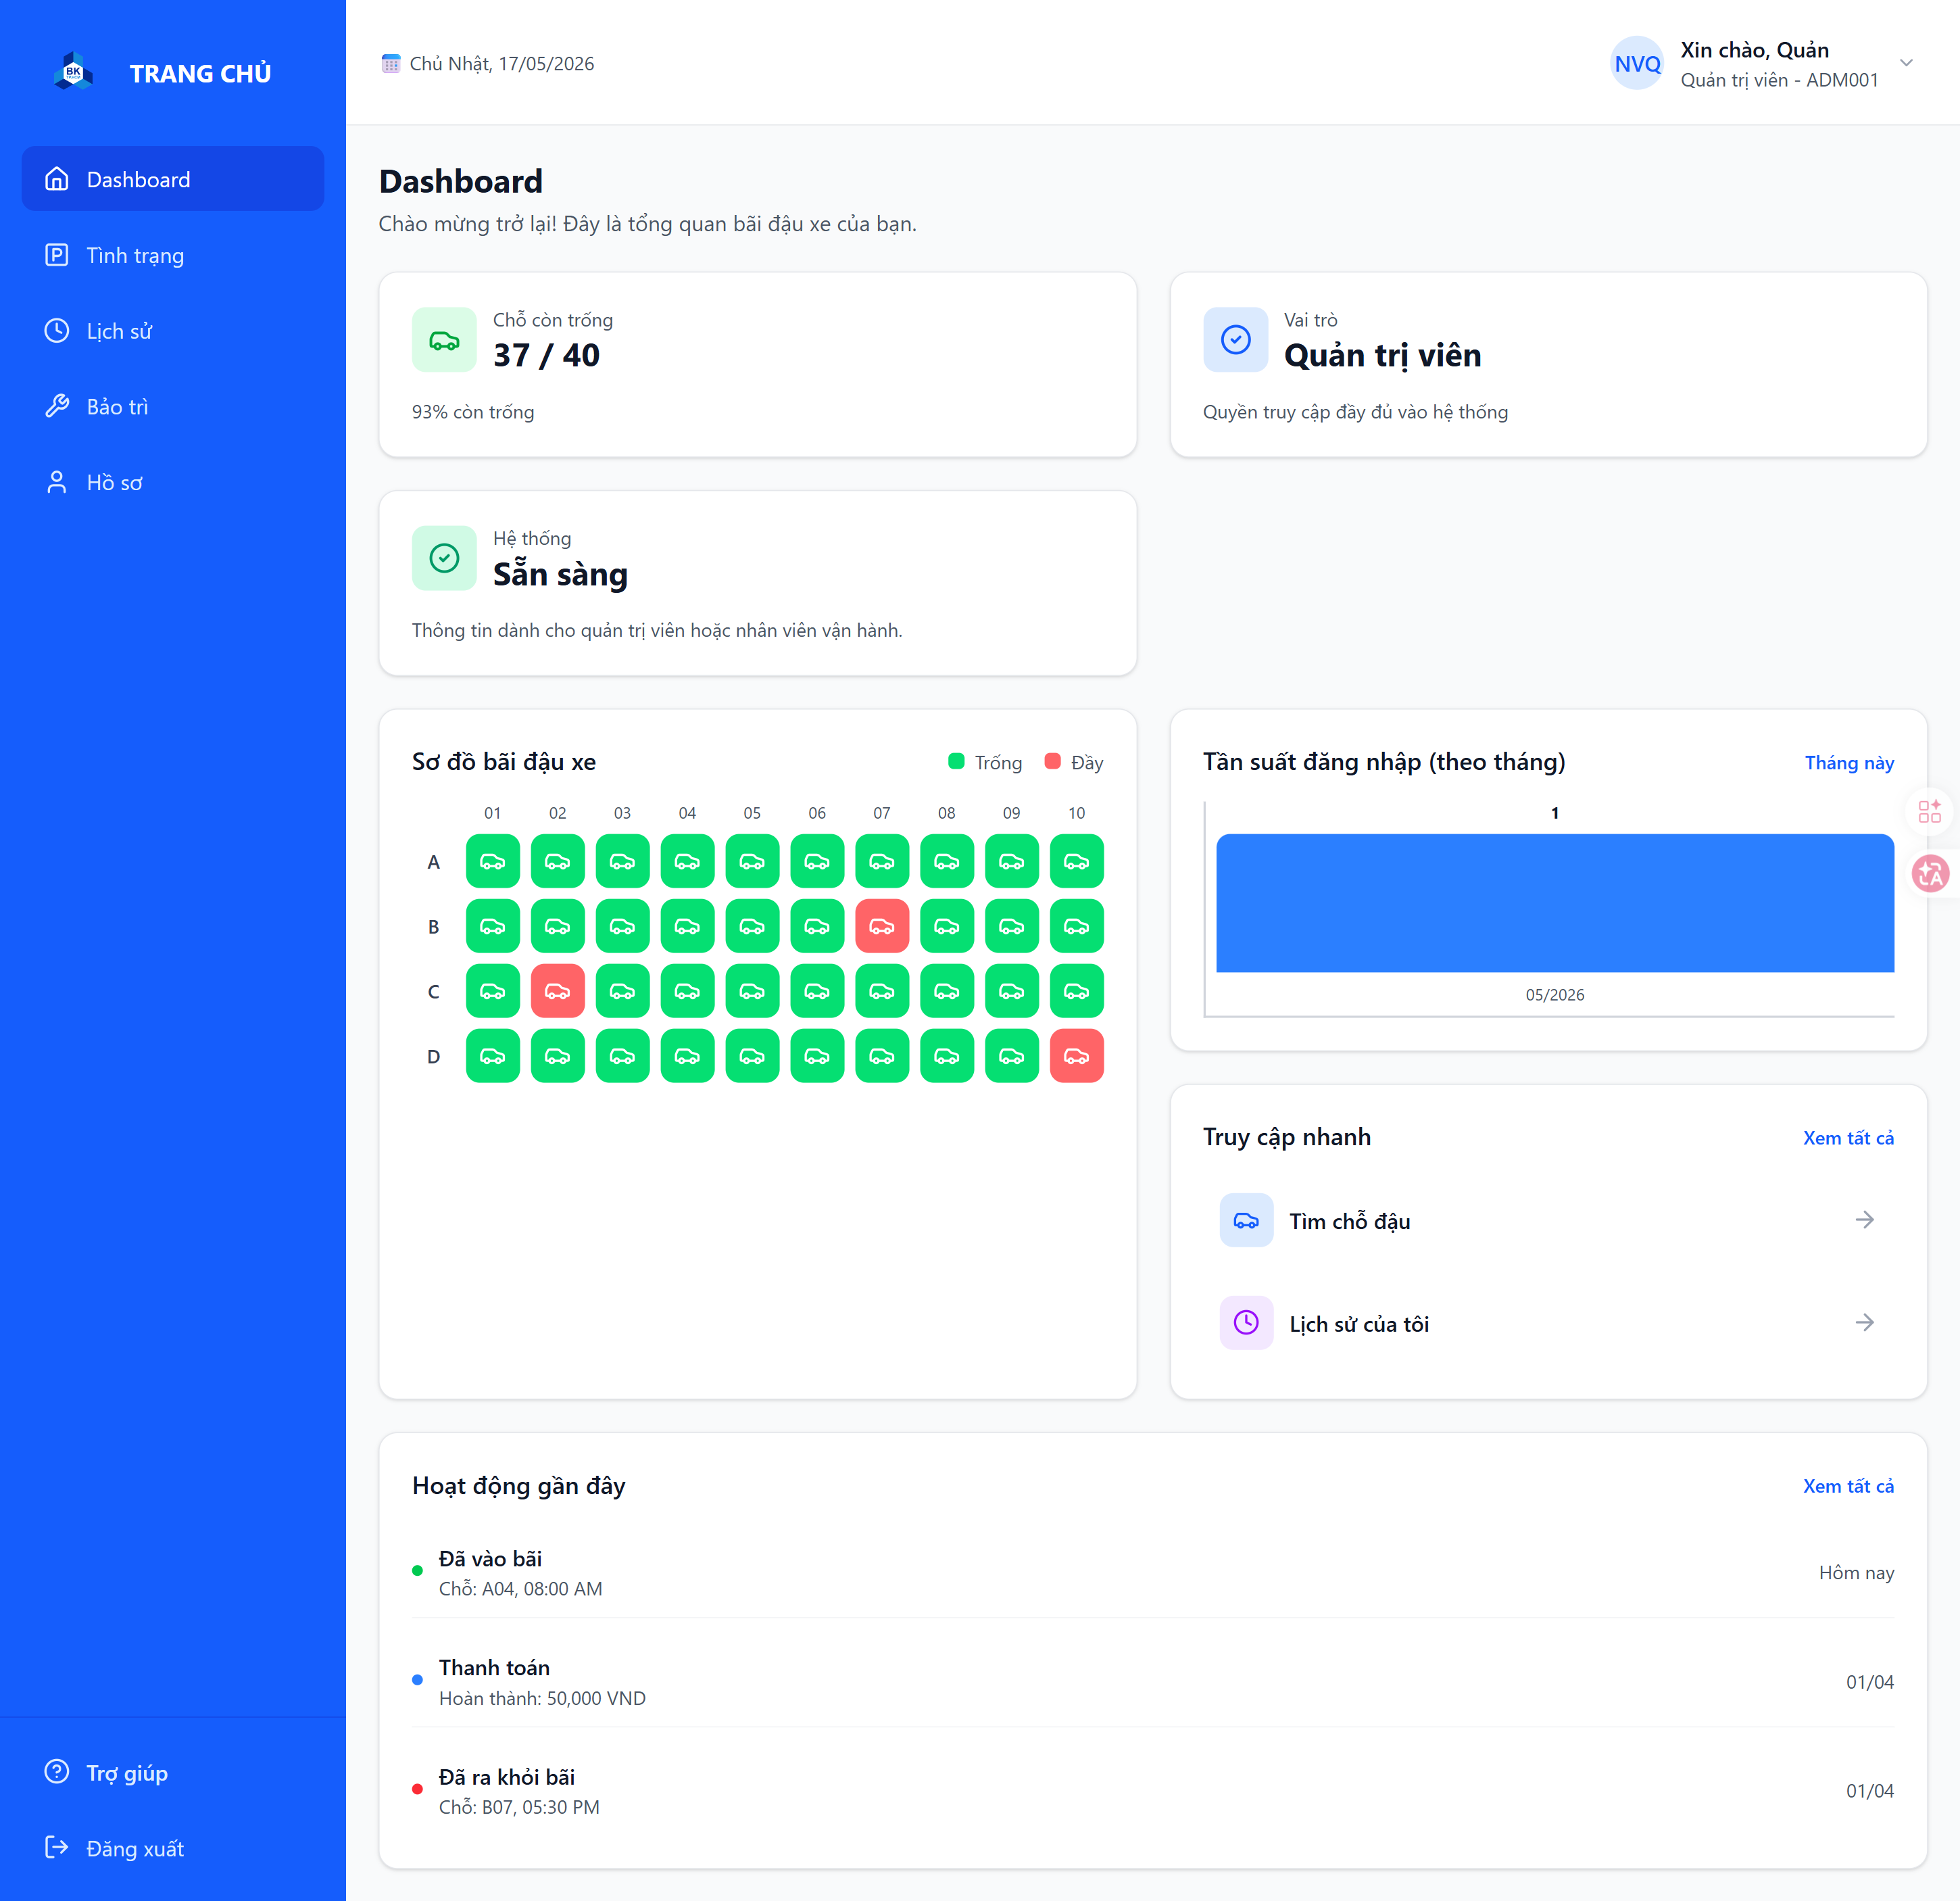
\includegraphics[width=1\linewidth]{Images/Task4/task4_admin_dashboard.png} 
	\caption{Dashboard tổng quan dành cho quản trị viên}
\end{figure}

\textbf{Bước 2.} Quản trị viên truy cập trang bảo trì để giám sát toàn bộ danh sách sự cố, lọc dữ liệu và cập nhật trạng thái từ chưa xử lý sang đang xử lý hoặc đã xử lý.

\begin{figure}[H]
	\centering
	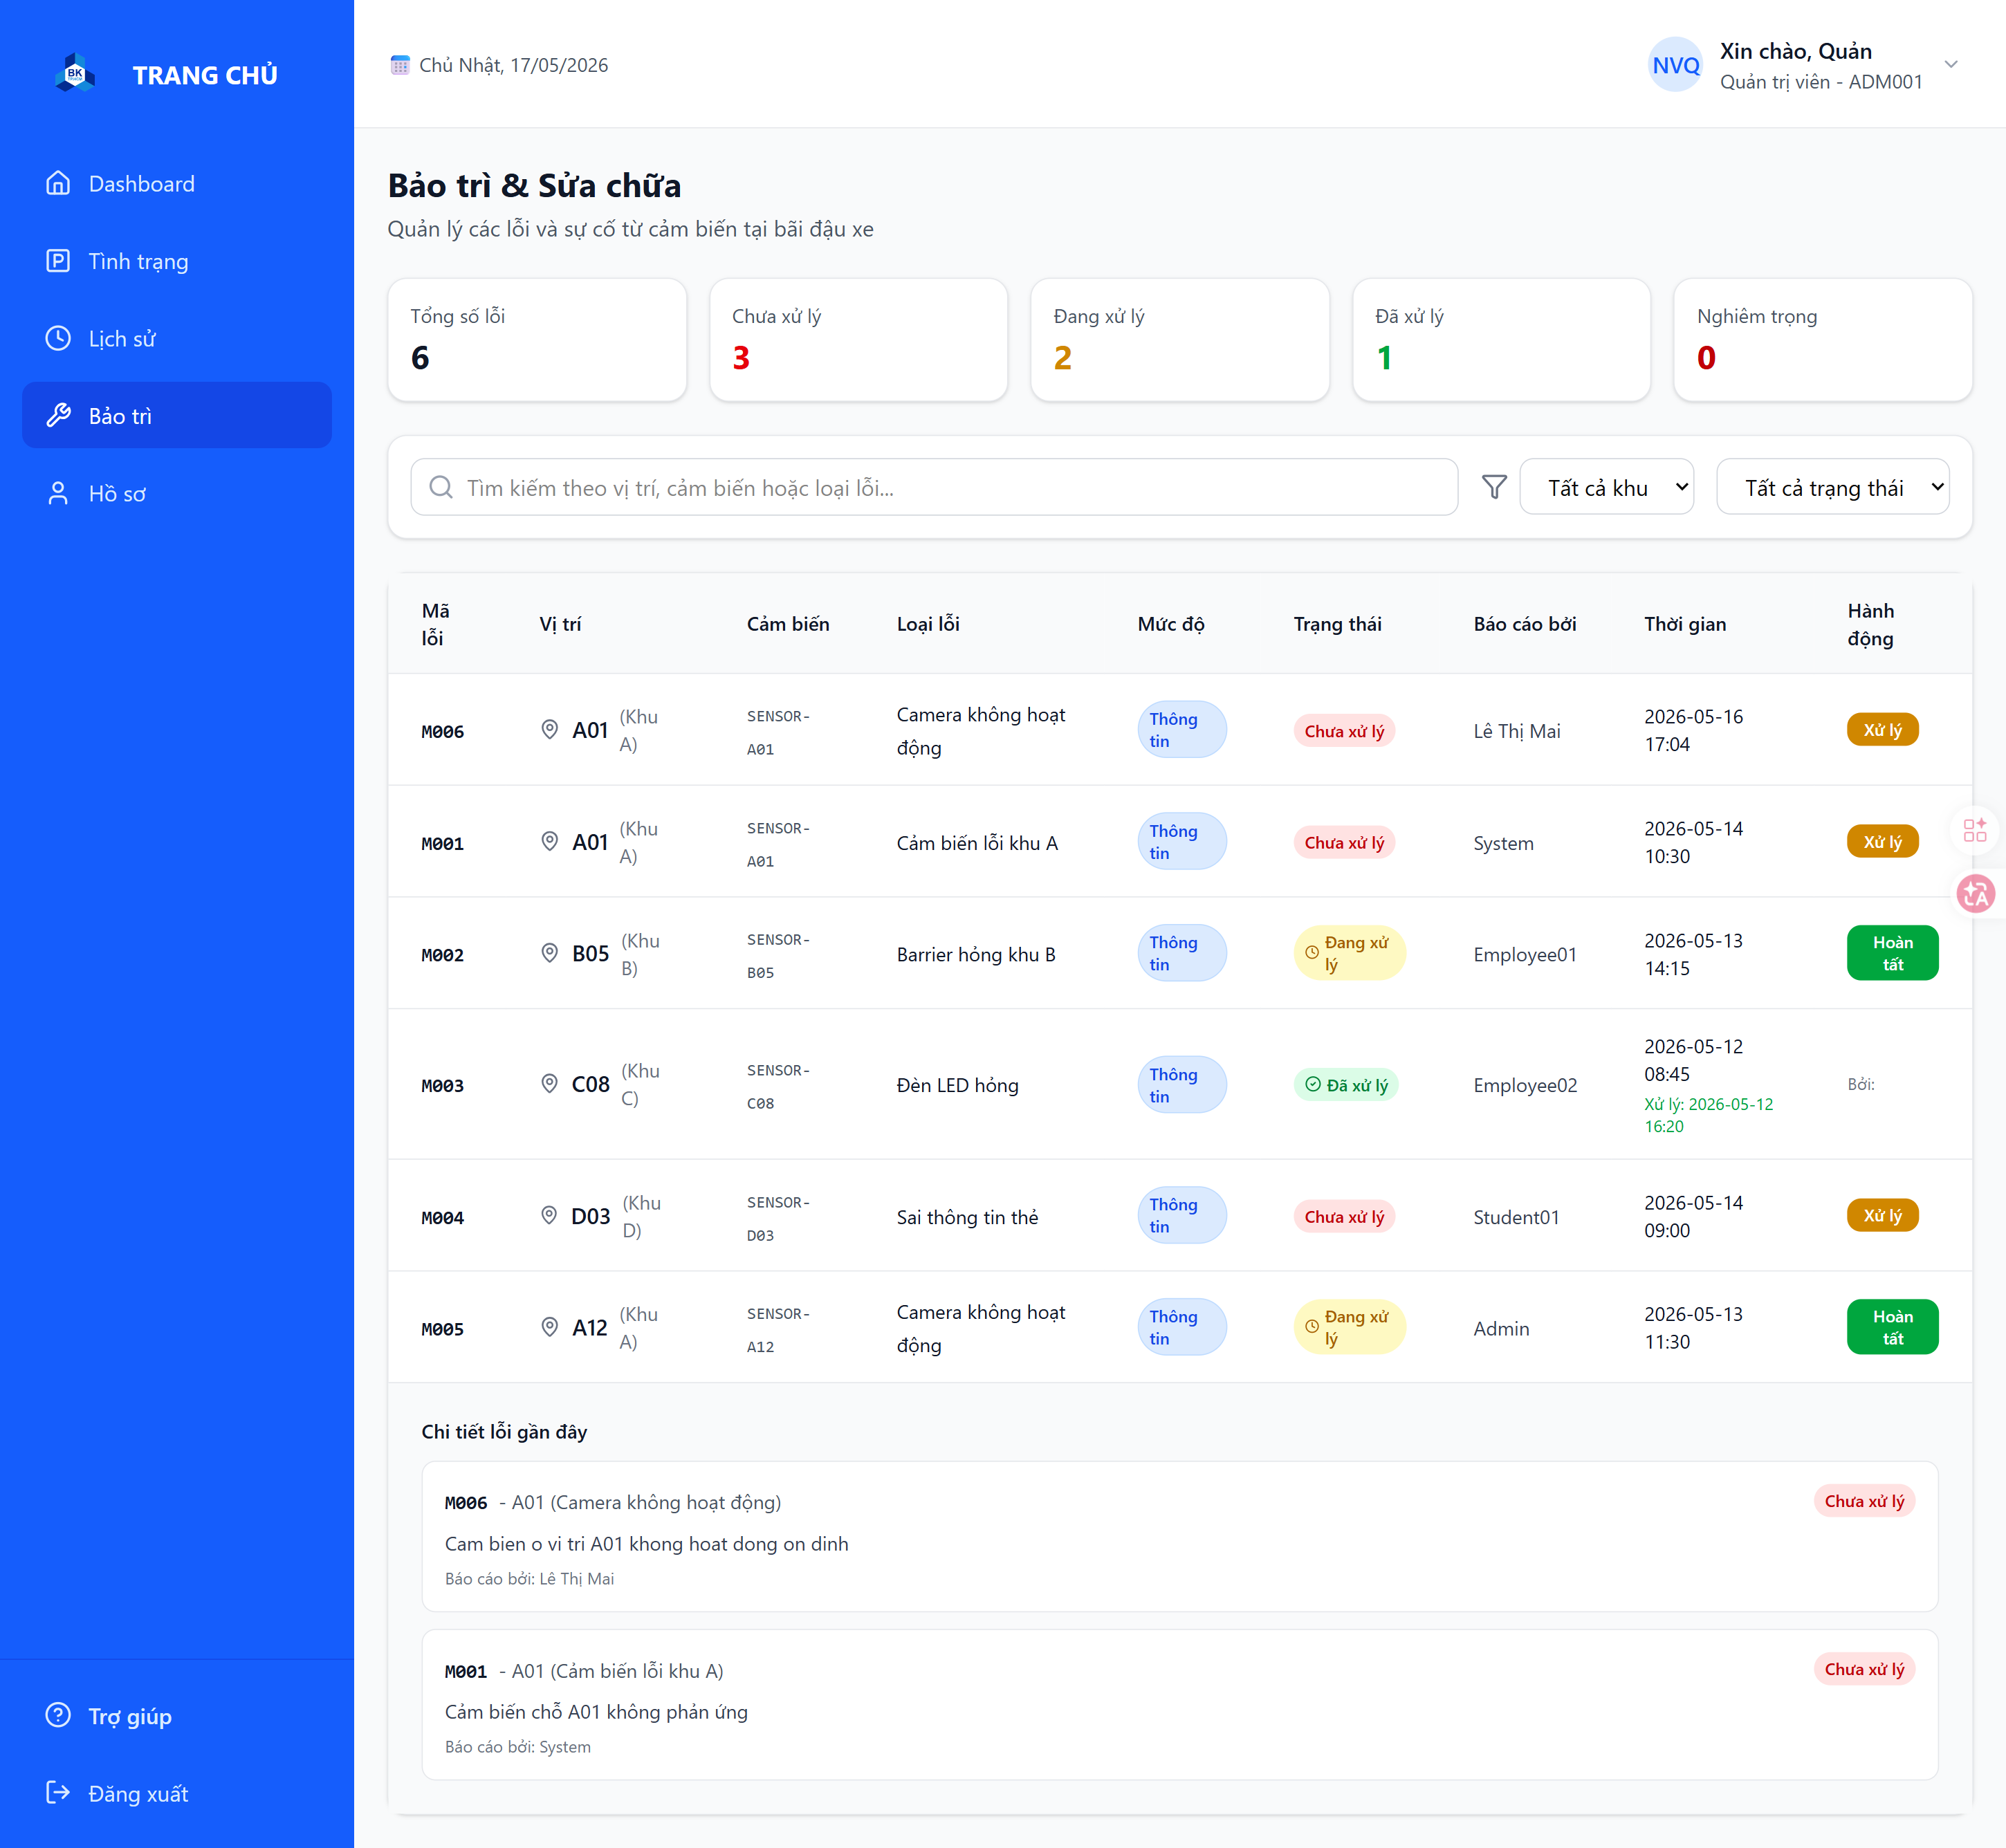
\includegraphics[width=1\linewidth]{Images/Task4/task4_admin_maintenance_management.png} 
	\caption{Trang quản lý sự cố của quản trị viên}
\end{figure}

\textbf{Bước 3.} Quản trị viên cũng có thể vào trang hồ sơ để kiểm tra thông tin tài khoản vận hành hệ thống và các tùy chọn bảo mật.

\begin{figure}[H]
	\centering
	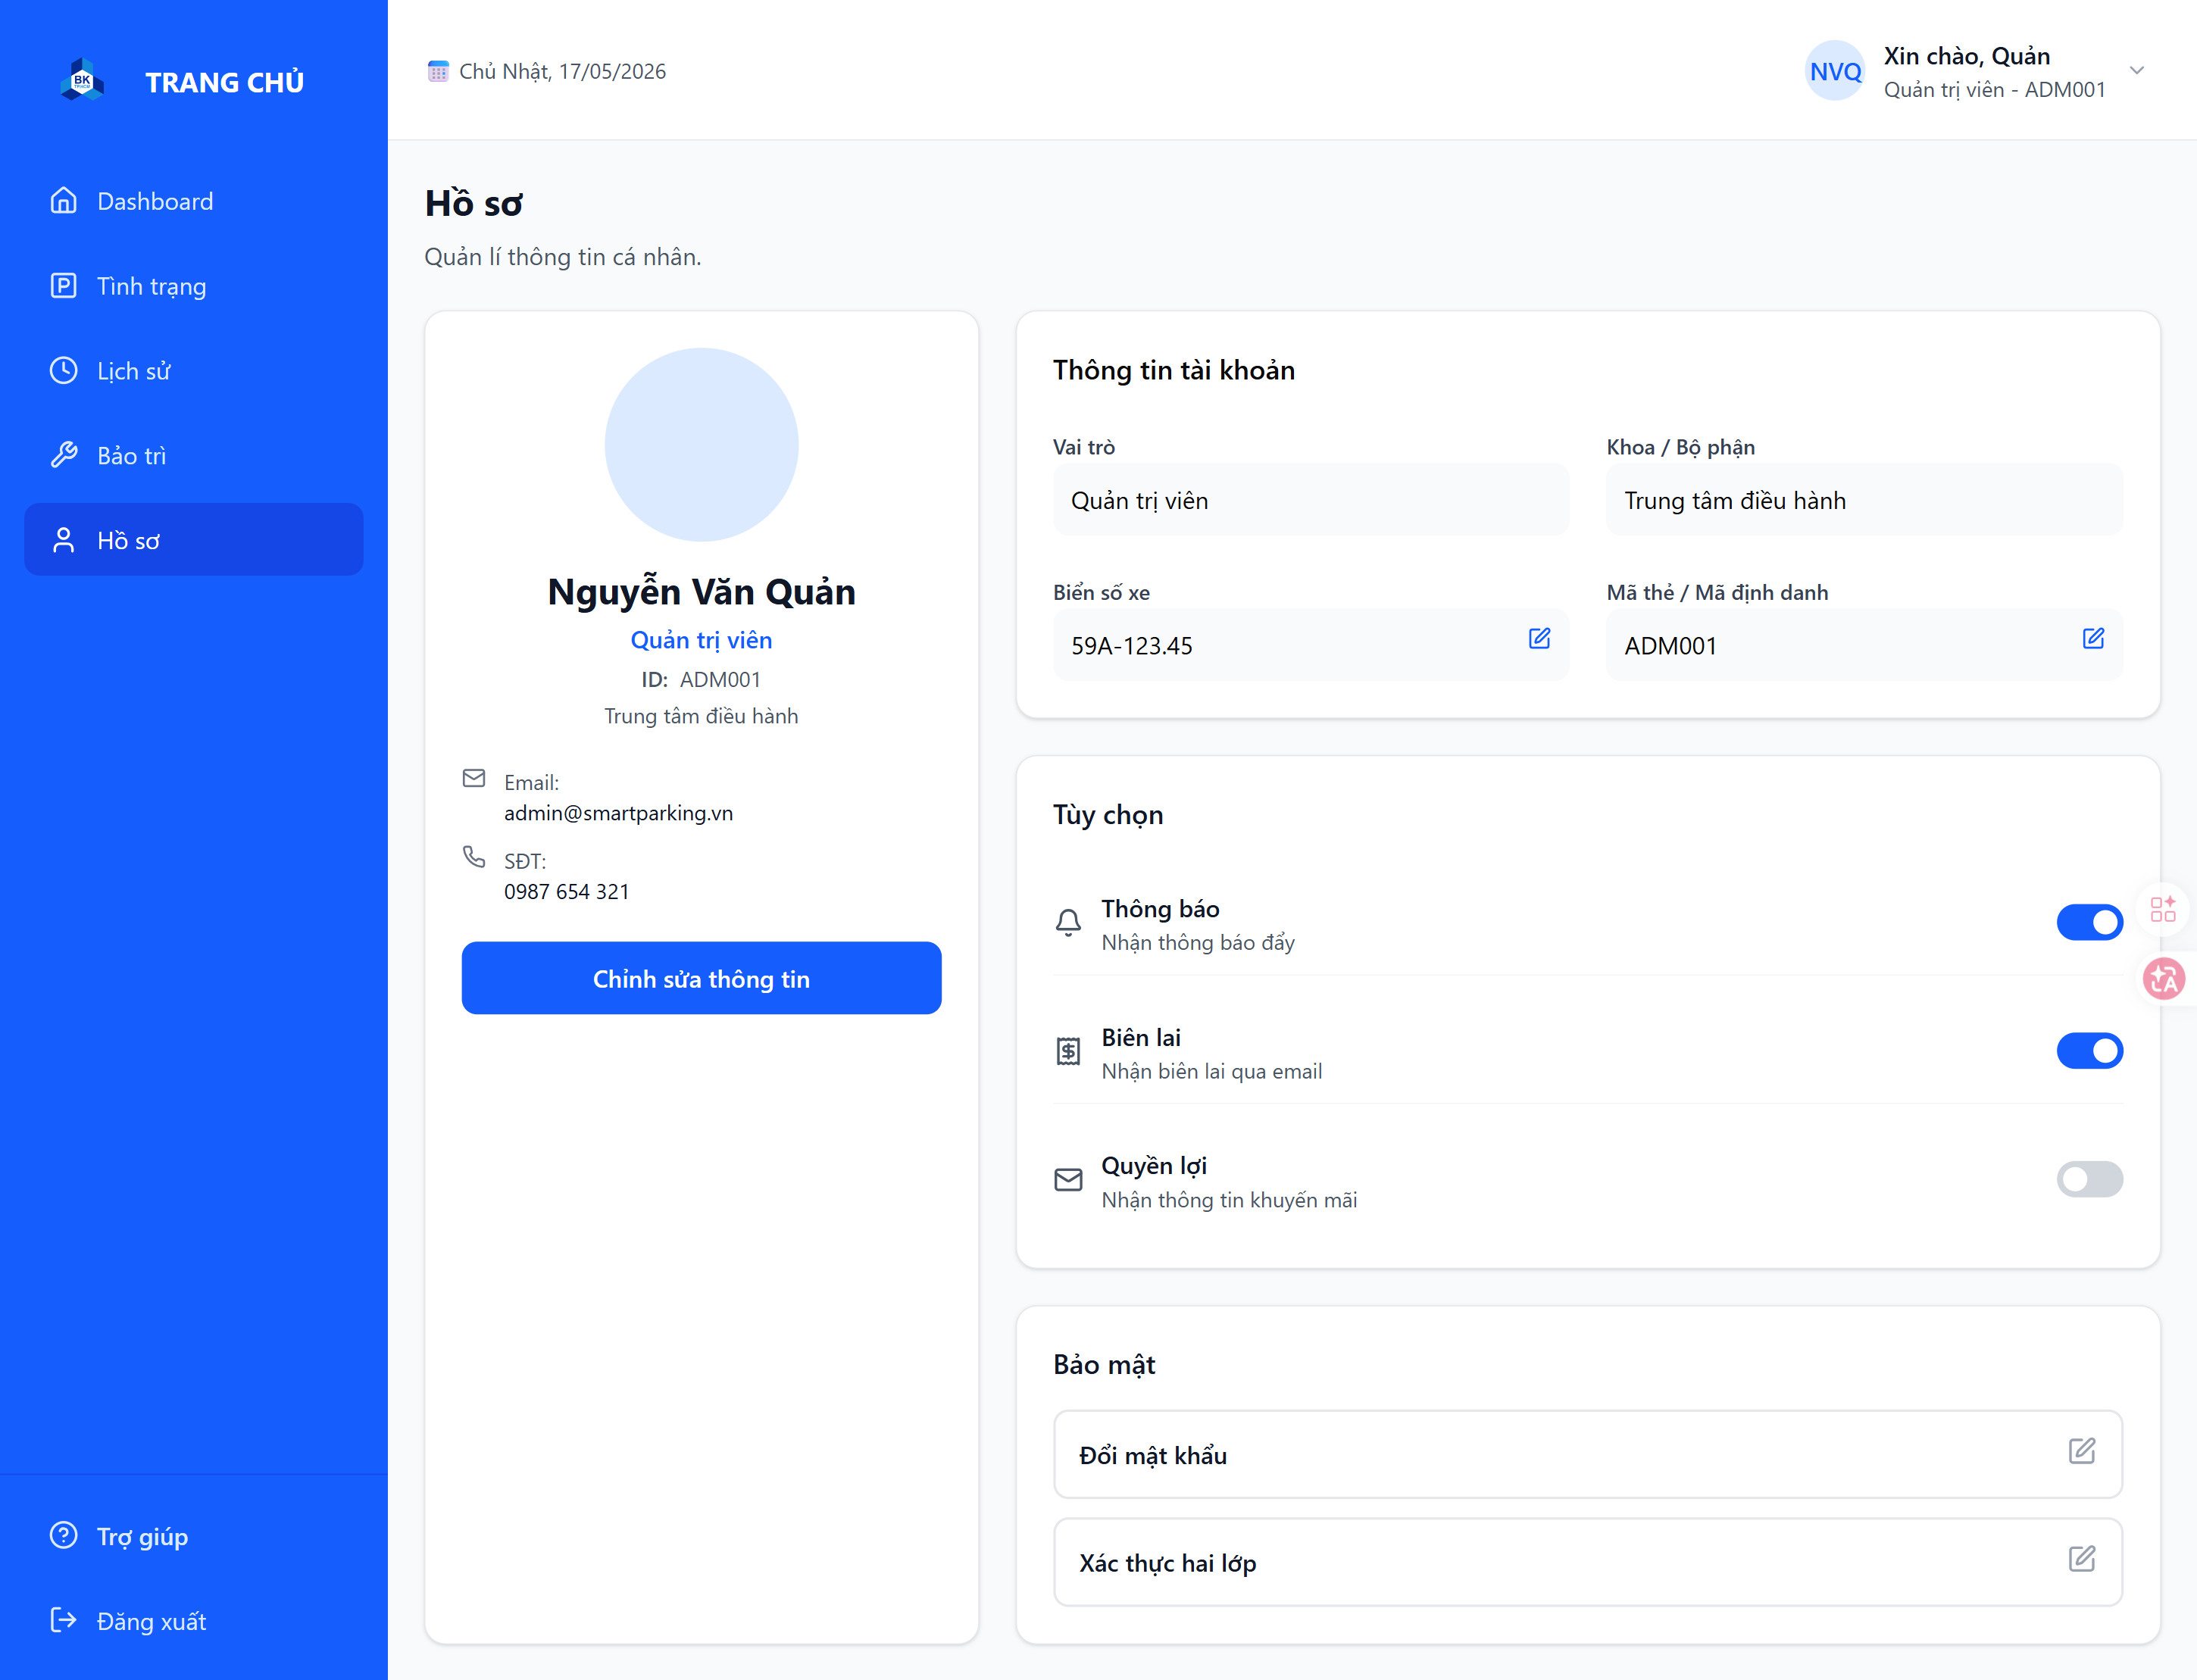
\includegraphics[width=1\linewidth]{Images/Task4/task4_admin_profile.png} 
	\caption{Trang hồ sơ của quản trị viên}
\end{figure}

\subsubsection{Kết luận cho phần working demonstration}

Thông qua chuỗi màn hình trên, phiên bản web hiện tại đã minh họa được các luồng sử dụng chính đã có trong mã nguồn: truy cập hệ thống, đăng nhập theo vai trò, theo dõi trạng thái bãi xe, mô phỏng check-in/check-out, thanh toán qua BKPay, xem lịch sử, quản lý hồ sơ và xử lý sự cố vận hành.

\newpage

\subsection{\textbf{Sử dụng Generative AI}}

Trong đồ án này, Generative AI được sử dụng như một công cụ hỗ trợ. Việc sử dụng được khai báo rõ ràng như sau:

\begin{itemize}
	\item \textbf{Công cụ sử dụng:} Nhóm có sử dụng các công cụ Generative AI để hỗ trợ gợi ý nội dung, hỗ trợ lập trình và hỗ trợ trình bày báo cáo.
	
	\item \textbf{Phạm vi sử dụng trong quá trình phát triển:}
	\begin{itemize}
		\item Gợi ý ý tưởng ban đầu cho giao diện và cách tổ chức chức năng của hệ thống web.
		\item Hỗ trợ sinh nháp mã cho một số phần frontend như trang đăng nhập, bố cục dashboard, bảng dữ liệu, biểu mẫu, popup thanh toán và một số giao diện liên quan đến bảo trì.
		\item Gợi ý cách tổ chức component, cấu trúc mã nguồn và cách kết nối các luồng giao diện với dữ liệu mô phỏng hoặc API.
		\item Hỗ trợ chỉnh sửa câu lệnh, cú pháp và cách trình bày mã trong quá trình hoàn thiện giao diện.
	\end{itemize}
	
	\item \textbf{Phạm vi sử dụng trong quá trình viết báo cáo:}
	\begin{itemize}
		\item Gợi ý cách tổ chức nội dung cho phần báo cáo.
		\item Hỗ trợ diễn đạt lại câu văn để nội dung rõ ràng, mạch lạc hơn.
		\item Hỗ trợ viết nháp cho phần mô tả luồng chức năng và phần working demonstration.
		\item Hỗ trợ rà soát, nhận xét và đối chiếu nội dung đã làm, ví dụ như danh sách use case, các luồng chức năng, các màn hình giao diện và mức độ đầy đủ giữa phần hiện thực với phần mô tả trong báo cáo.
		\item Hỗ trợ định dạng nội dung bằng \LaTeX{}.
	\end{itemize}
	
	\item \textbf{Mức độ đóng góp của AI:} AI chỉ đóng vai trò hỗ trợ trong việc gợi ý, tạo nháp và tăng tốc quá trình thực hiện. AI không được sử dụng như nguồn đầu ra cuối cùng mà không qua kiểm tra.
	
	\item \textbf{Phần công việc do nhóm tự thực hiện:}
	\begin{itemize}
		\item Tự đọc và phân tích yêu cầu của đồ án.
		\item Tự chọn lọc, chỉnh sửa và tích hợp các phần gợi ý từ AI vào hệ thống.
		\item Tự kiểm tra lại mã nguồn, luồng chức năng và giao diện thực tế của web.
		\item Tự chụp ảnh minh họa, đối chiếu nội dung báo cáo với hệ thống đang chạy và hoàn thiện bản nộp cuối cùng.
	\end{itemize}
	
	\item \textbf{Trách nhiệm học thuật:} Nhóm chịu trách nhiệm hoàn toàn đối với phần hiện thực, phần phân tích và toàn bộ nội dung báo cáo đã nộp. Mọi nội dung do AI hỗ trợ đều đã được nhóm xem xét, chỉnh sửa và xác nhận lại trước khi sử dụng.
\end{itemize}

Vì vậy, Generative AI chỉ đóng vai trò là công cụ hỗ trợ trong việc tìm ý tưởng, tạo nháp và tăng tốc quá trình làm việc. Nhóm chịu trách nhiệm hoàn toàn đối với phần hiện thực, phần phân tích và nội dung báo cáo đã nộp.

\newpage

\section{Tài liệu tham khảo}

\begin{enumerate}
	\item Object Management Group (OMG), \textit{OMG Unified Modeling Language (OMG UML), Version 2.5.1}, 2017. Truy cập tại: \texttt{https://www.omg.org/spec/UML/2.5.1/PDF}

	\item IEEE Computer Society, \textit{Guide to the Software Engineering Body of Knowledge (SWEBOK Guide)}. Truy cập tại: \texttt{https://www.computer.org/education/bodies-of-knowledge/software-engineering}
	
	\item Ian Sommerville, \textit{Software Engineering}, 10th Edition, Pearson, 2015.
\end{enumerate}

